% https://github.com/martinhelso/MathDept


\documentclass[UKenglish]{beamer}


\usetheme[NoLogo]{MathDept}


\usepackage[utf8]{inputenx} % For æ, ø, å
\usepackage{babel}          % Automatic translations
\usepackage{csquotes}       % Quotation marks
\usepackage{microtype}      % Improved typography
\usepackage{amssymb}        % Mathematical symbols
\usepackage{mathtools}      % Mathematical symbols
\usepackage[absolute, overlay]{textpos} % Arbitrary placement
\setlength{\TPHorizModule}{\paperwidth} % Textpos units
\setlength{\TPVertModule}{\paperheight} % Textpos units
\usepackage{tikz}
\usepackage{diagbox}
\usetikzlibrary{overlay-beamer-styles}  % Overlay effects for TikZ

\author{William Hirst}
\title[Supervised Learning in HEP]{Application of Supervised Machine Learning to the Search for New Physics in ATLAS data}
\subtitle{A Study of Ordinary Dense, Parameterized and Ensemble Networks and their Application to High Energy Physics}


\begin{document}


\begin{frame}{Outline}
    \tableofcontents
\end{frame}


\section{Introduction $\&$ Motivation}
\begin{frame}{Introduction $\&$ Motivation}
    \tableofcontents[currentsection]
\end{frame}

\begin{frame}{Why apply machine learning to HEP problems?}
    \begin{itemize}
        \item The standard model (SM) of \\particle physics is very\\ successful, but not complete
        \begin{itemize}
            \item Neutrino masses 
            \item Hierarchy problem 
        \end{itemize}
        \item Large amount of data
        \item Machine learning (ML)
        \begin{itemize}
            \item Event reconstruction
            \item Particle classification
            \item Creating search regions
        \end{itemize}
    \end{itemize}
    \begin{textblock}{1}(0.5475,0.16)
        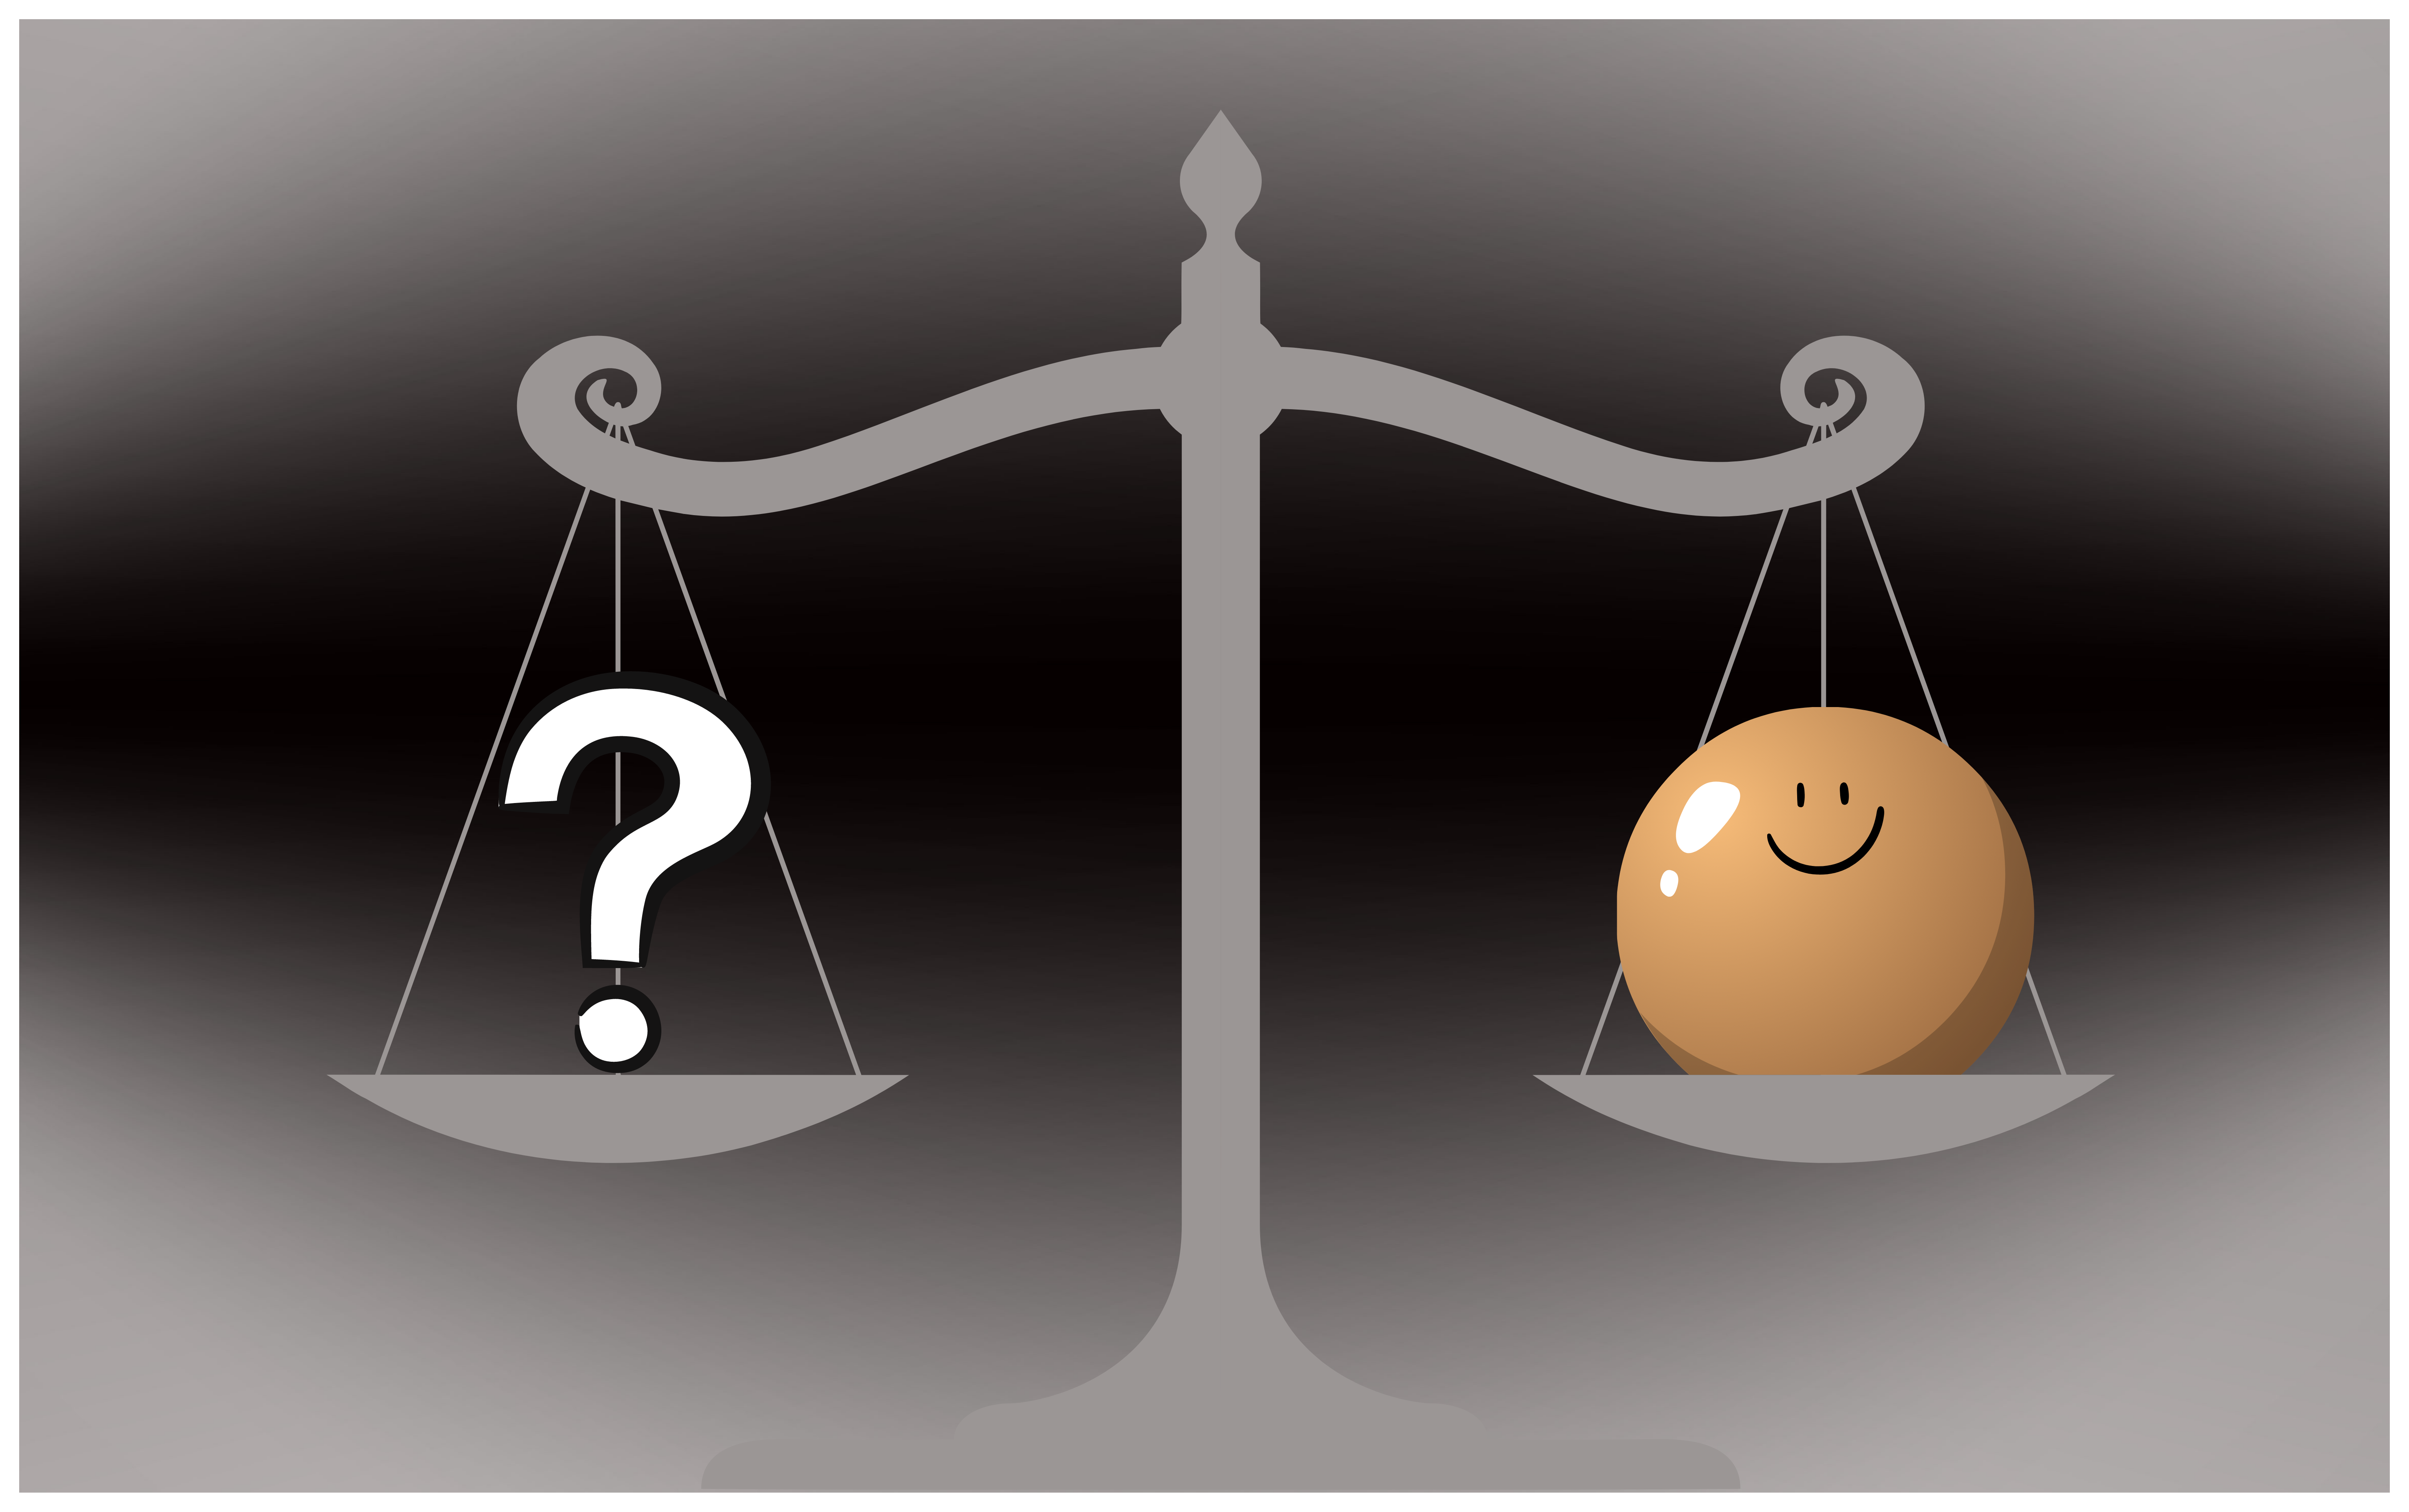
\includegraphics[width=0.375\textwidth]{figures/neutrino}
    \end{textblock}
    \begin{textblock}{1}(0.55,0.5)
        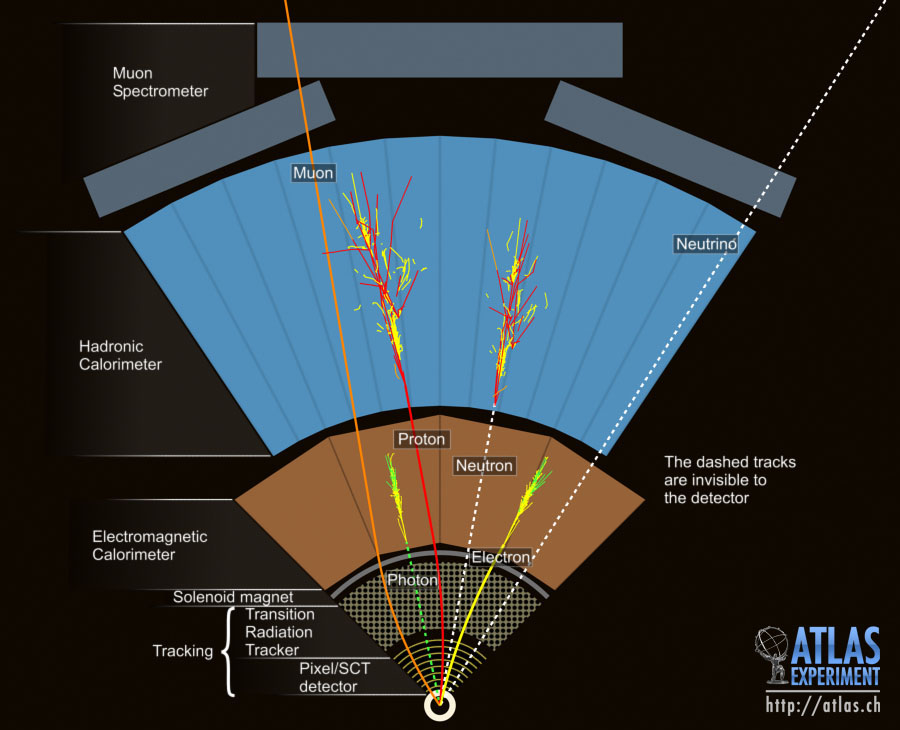
\includegraphics[width=0.37\textwidth]{figures/detector}
    \end{textblock}
\end{frame}

\begin{frame}{How do we search for new physics?}

    \begin{textblock}{1}(0.45, 0.55)
        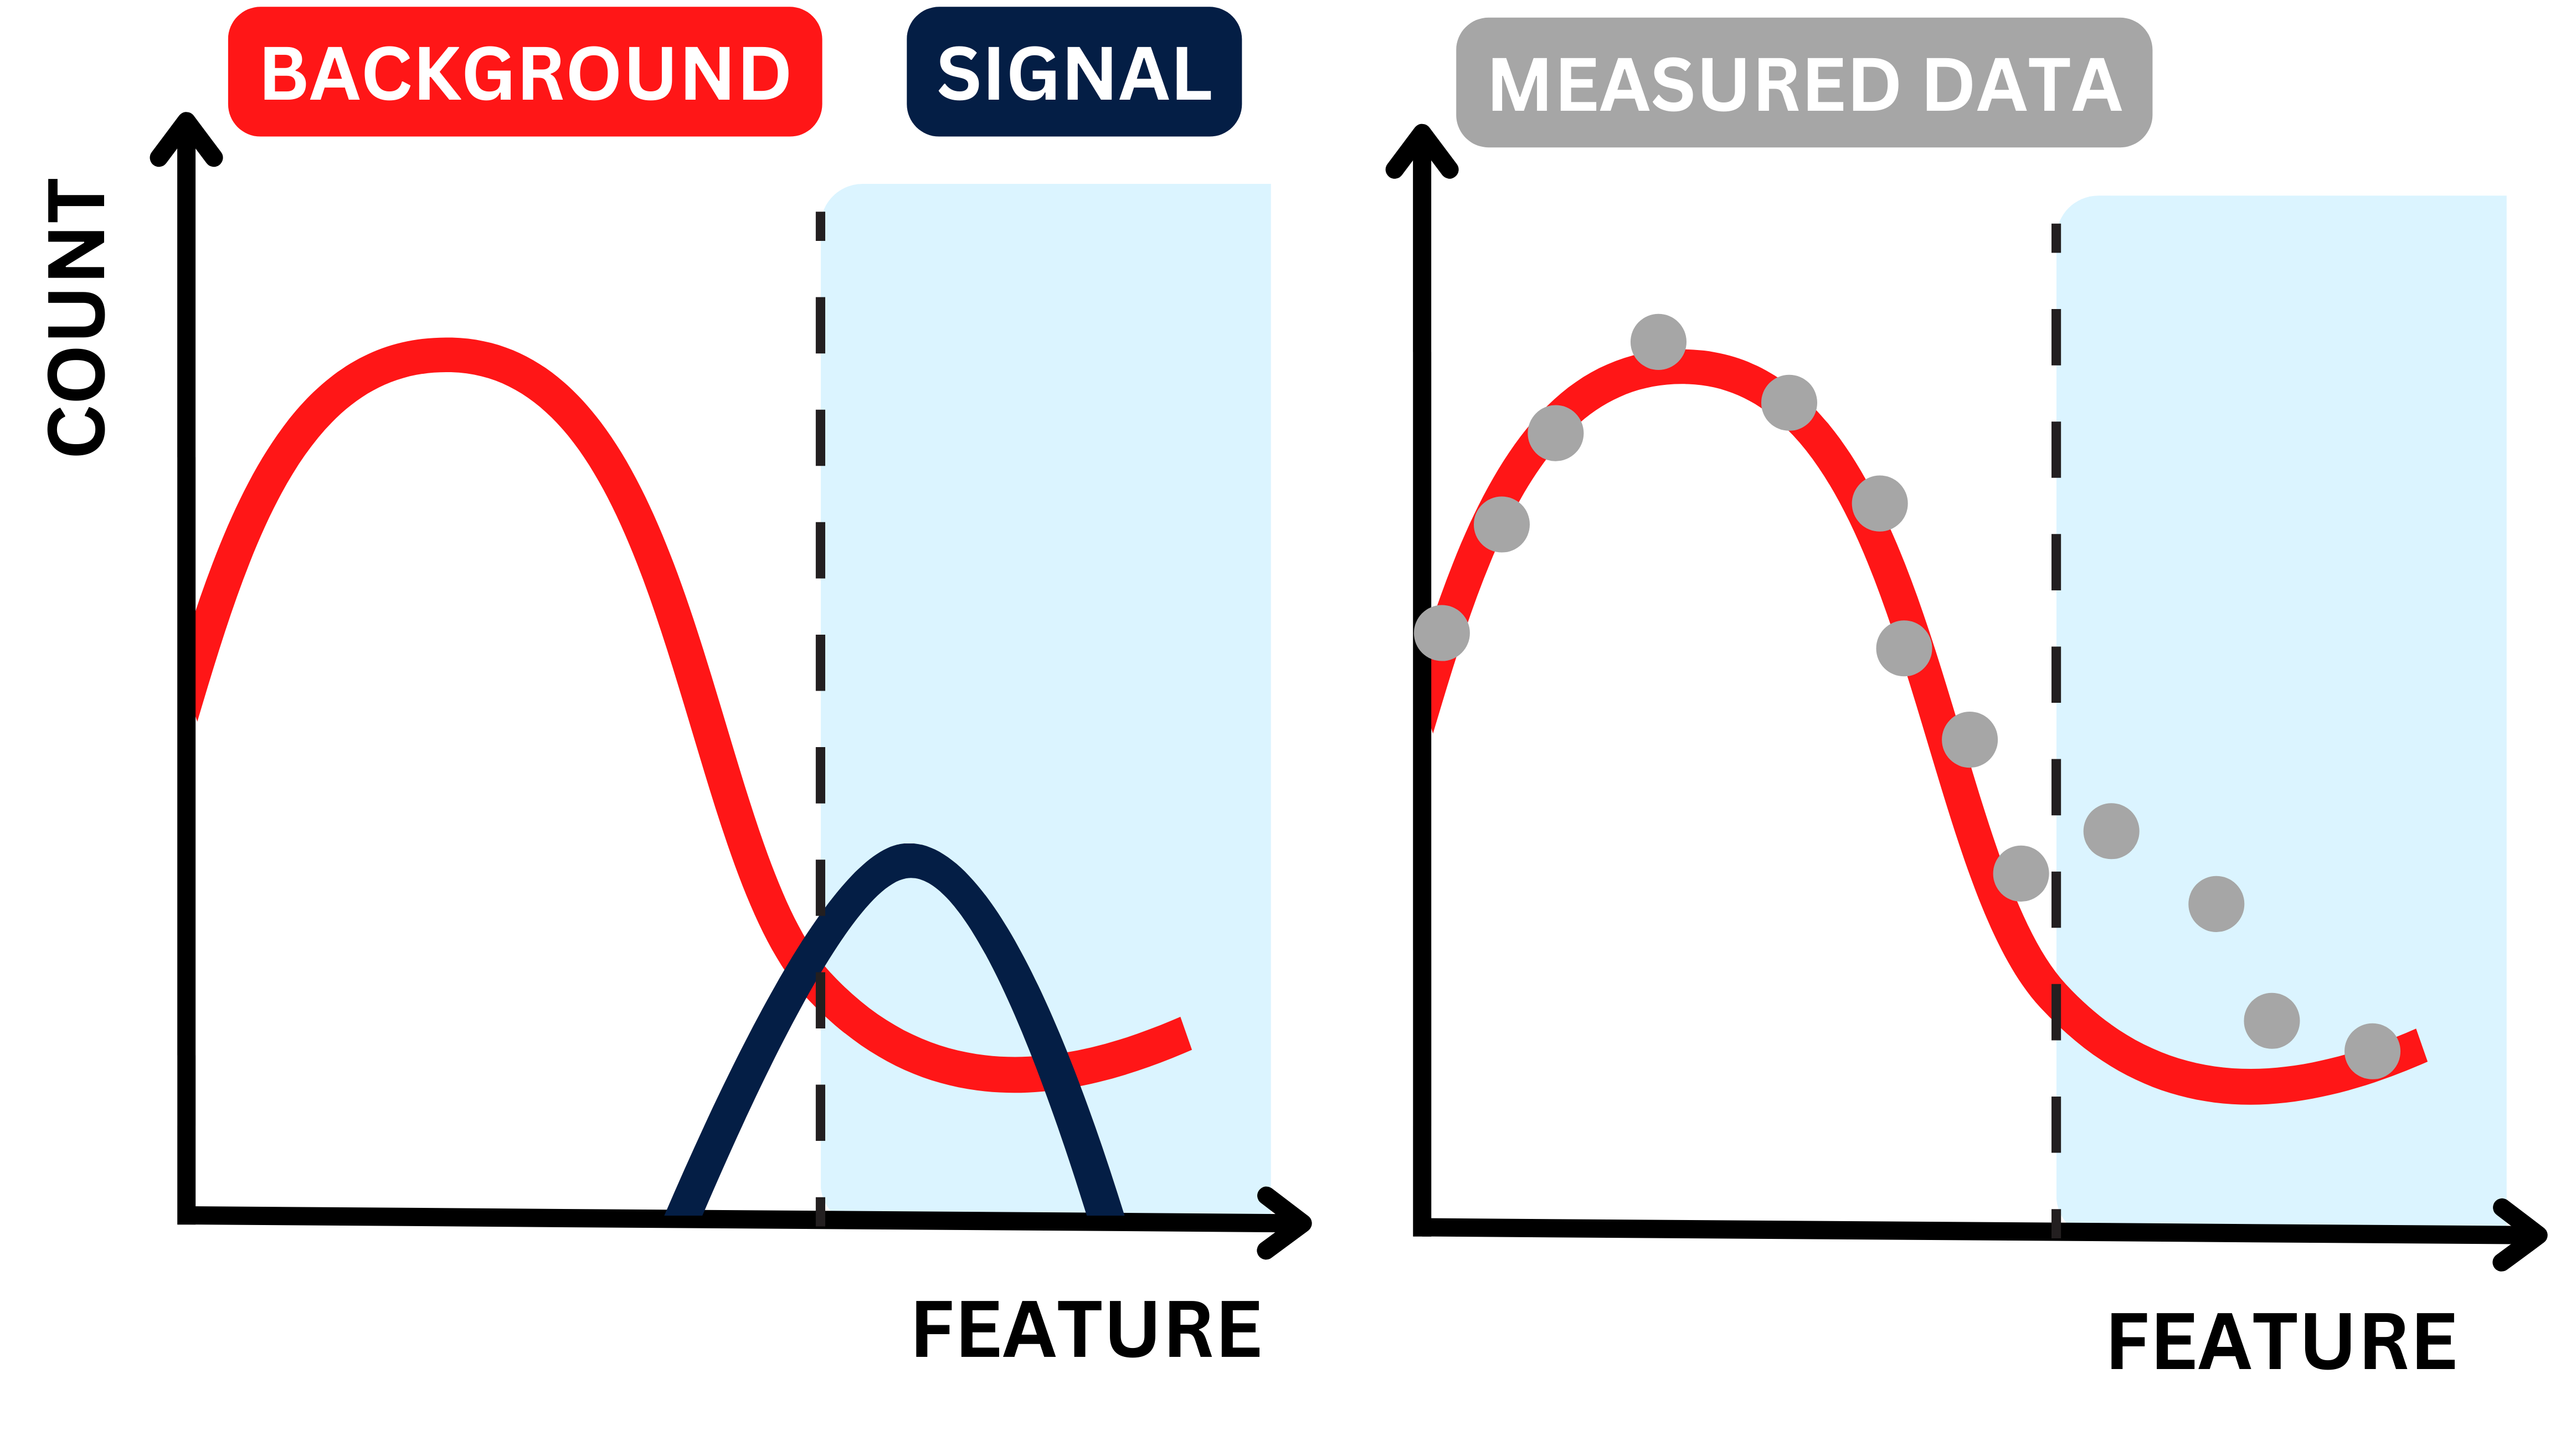
\includegraphics[width = 0.5\textwidth]{figures/DataCompHalf.png}
    \end{textblock}
    \begin{textblock}{1}(0.49, 0.15)
        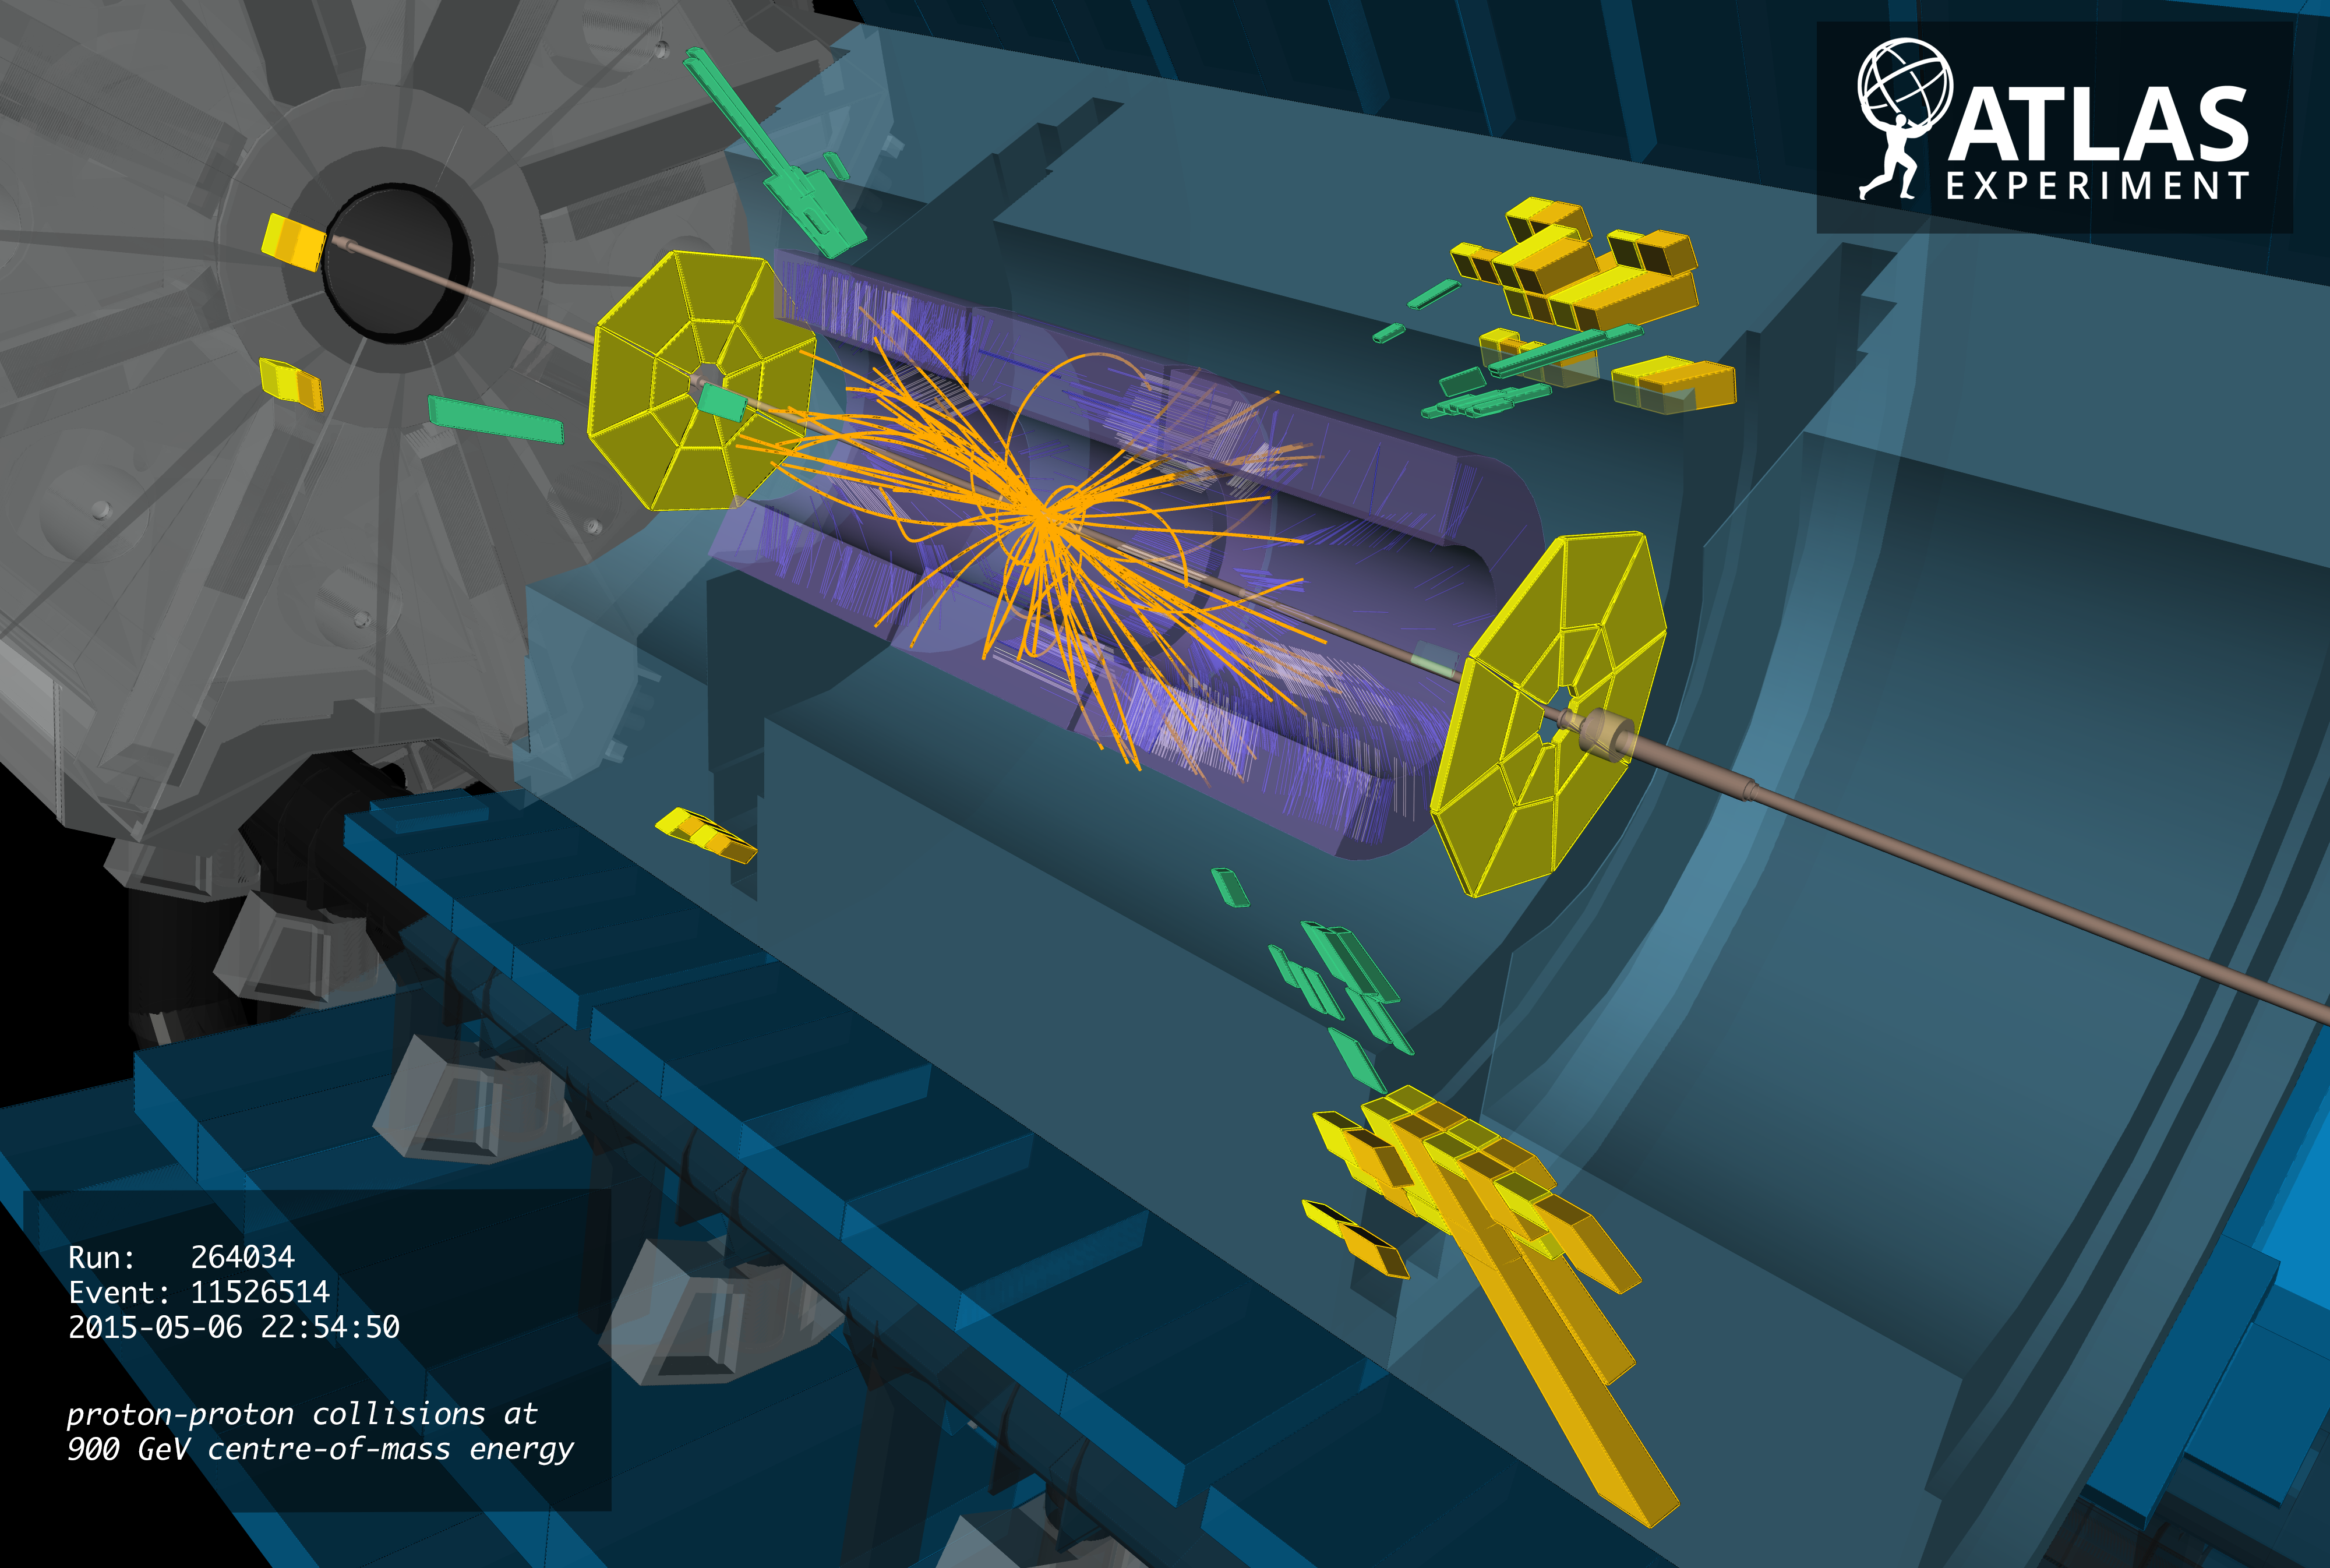
\includegraphics[width = 0.425\textwidth]{figures/vp1_3dcocktail_run264034_evt11526514_2015-05-06T22-54-50_2}
    \end{textblock}
    \begin{textblock}{0.45}(0., 0.18)
        \begin{itemize}
            \item Compare theory with experiment 
            \begin{itemize}
                \item Experiment: Measured
                \item Theory: Simulated (background and signal)
            \end{itemize}
            \item Search regions
            \item Expected significance
            \begin{itemize}
                \item $Z_{exp}\approx \frac{signal}{\sqrt{background}}$
            \end{itemize}
            \item Difficult to separate $\rightarrow$ ML
        \end{itemize}
    \end{textblock}
\end{frame}
% \begin{frame}{How do we search for new physics?}
%     \begin{textblock}{1}(0.45, 0.475)
%         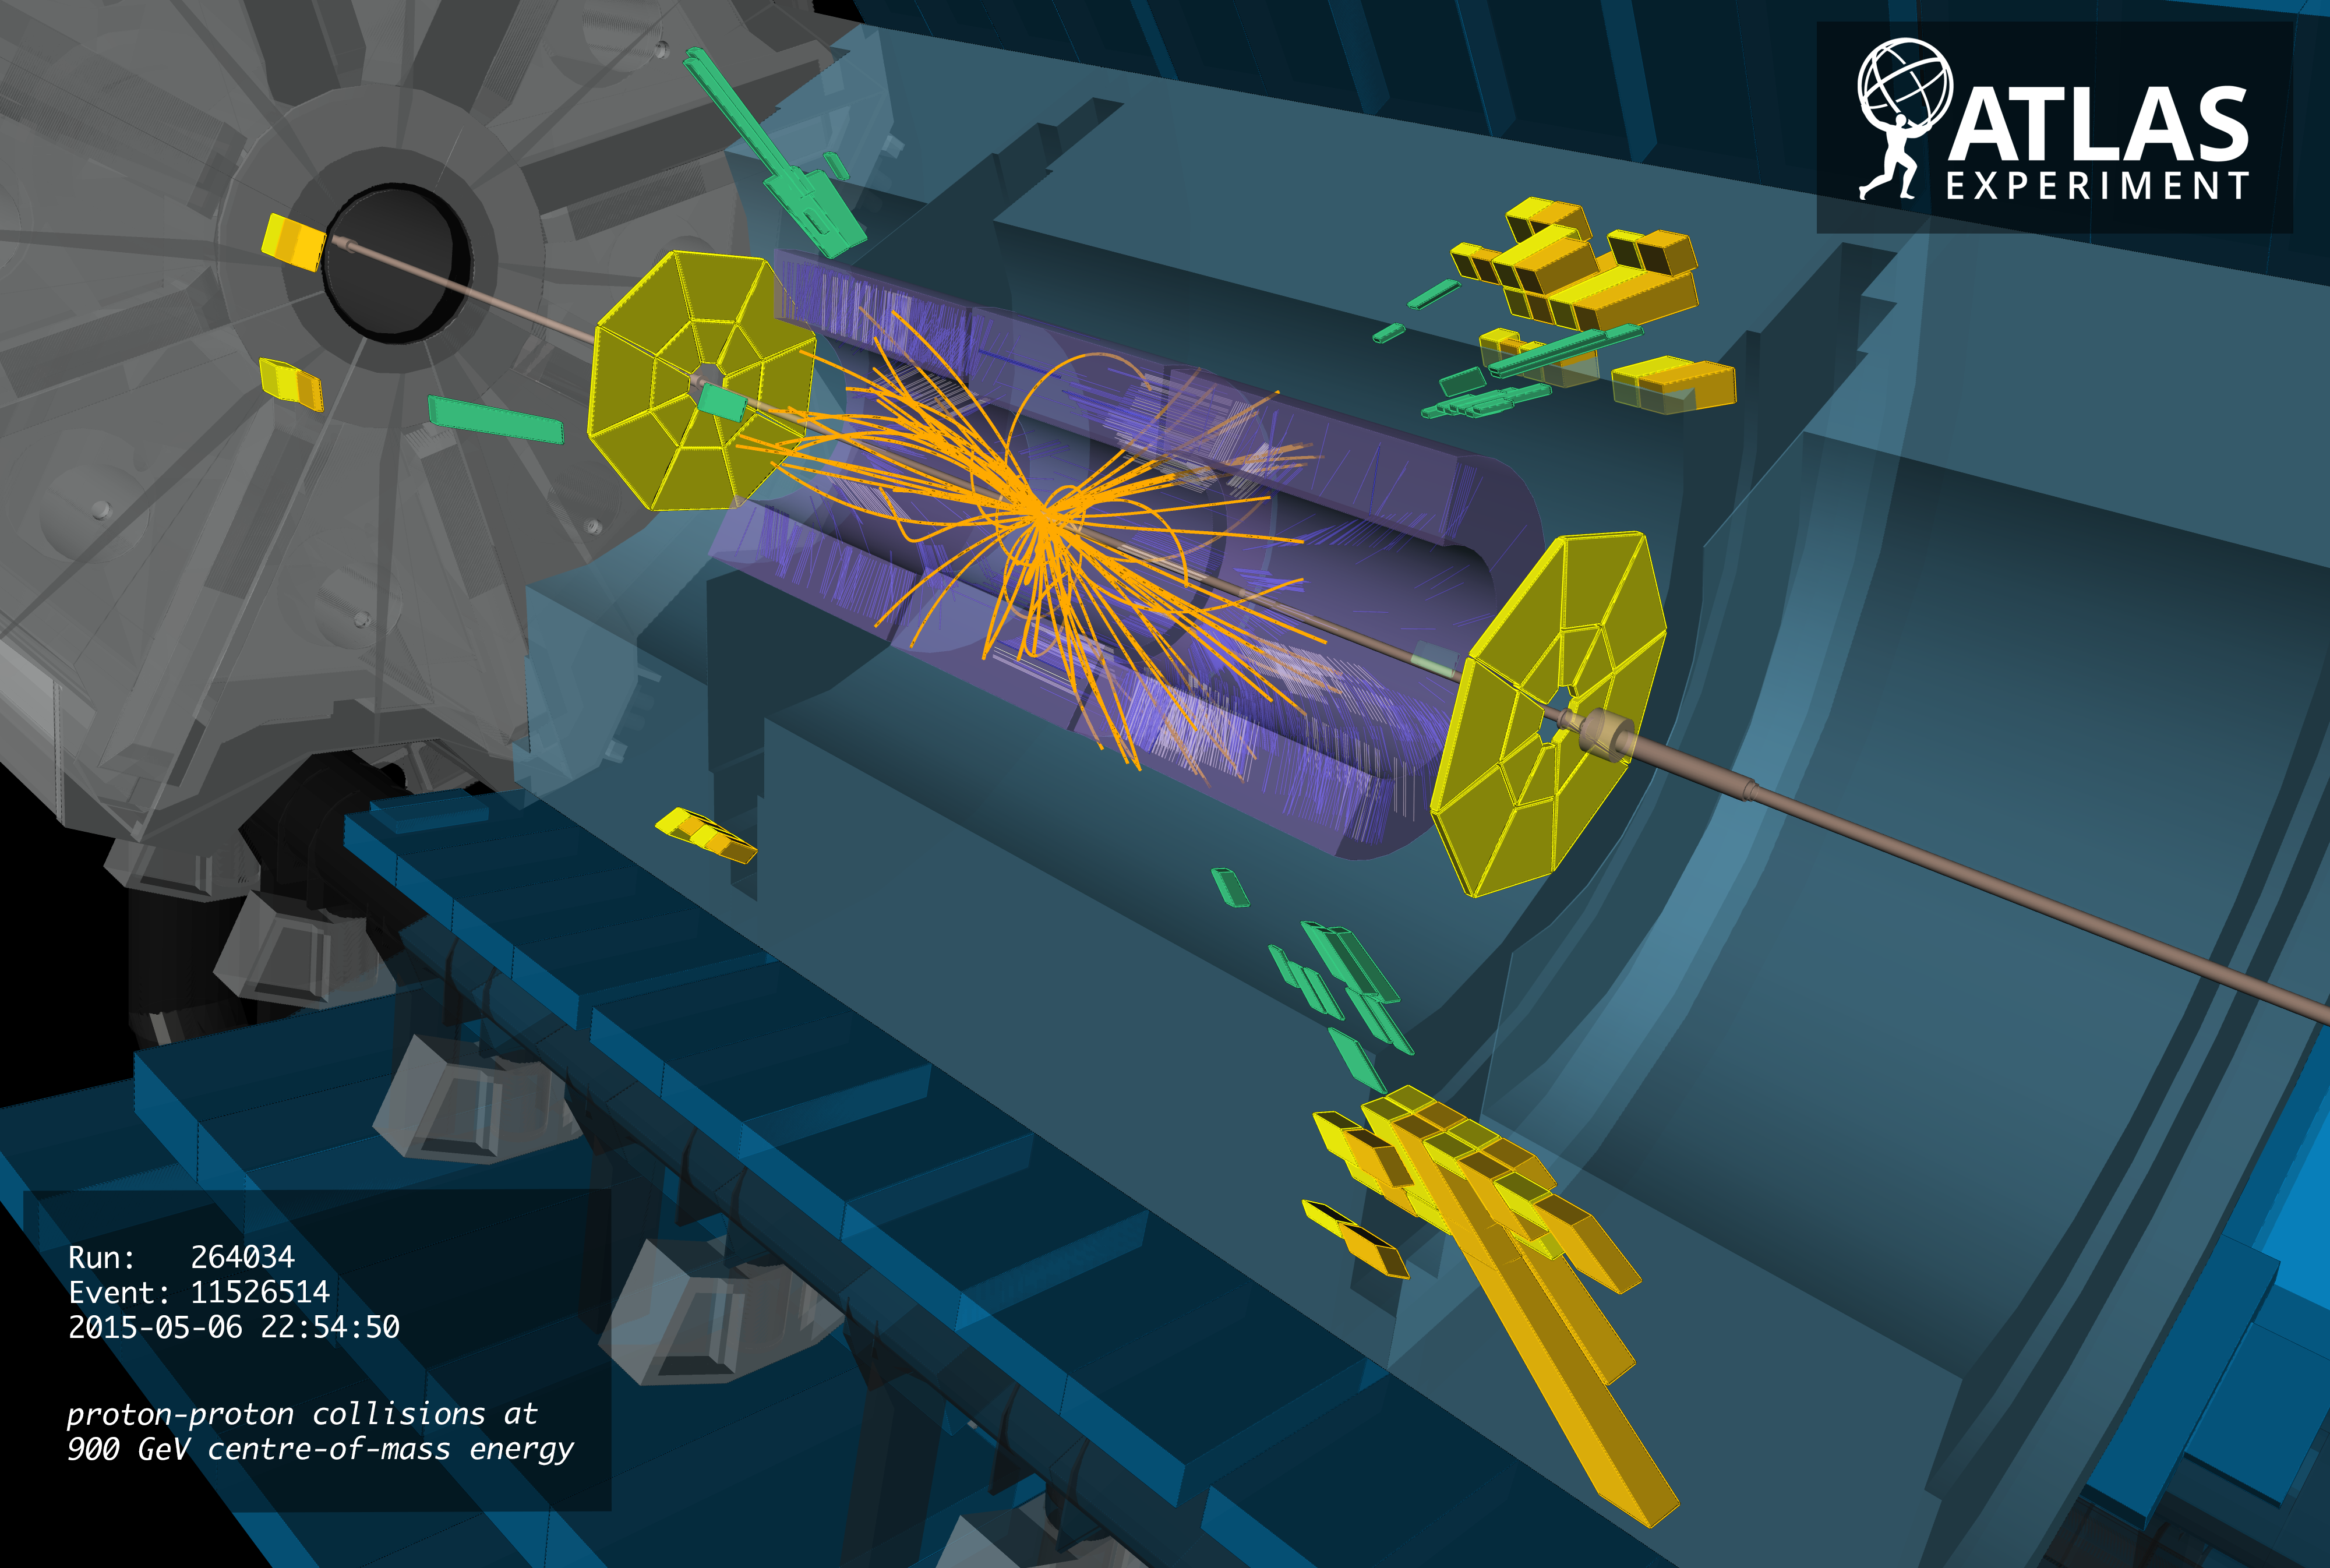
\includegraphics[width=0.5\textwidth]{figures/vp1_3dcocktail_run264034_evt11526514_2015-05-06T22-54-50_2}
%     \end{textblock}
%     \begin{itemize}
%         \item Compare theory with experiment 
%         \begin{itemize}
%             \item Experiment: Proton-proton collisions produced at the LHC and measured in the ATLAS detectors
%             \item Theory: Simulated based on SM physics 
%         \end{itemize}
%         \item Deviations $\rightarrow$ New physics (?) 
%         \item Measure deviation in significance
%         \begin{itemize}
%             \item $Z_{obs}\approx \frac{n_{obs} - bkg_{sim}}{\sqrt{bkg_{sim}}}$
%             \item $Z_{exp}\approx \frac{sgn_{sim}}{\sqrt{bkg_{sim}}}$
%         \end{itemize}
%     \end{itemize}

% \end{frame}
% \begin{frame}
%     \vfill
%     \centering
%     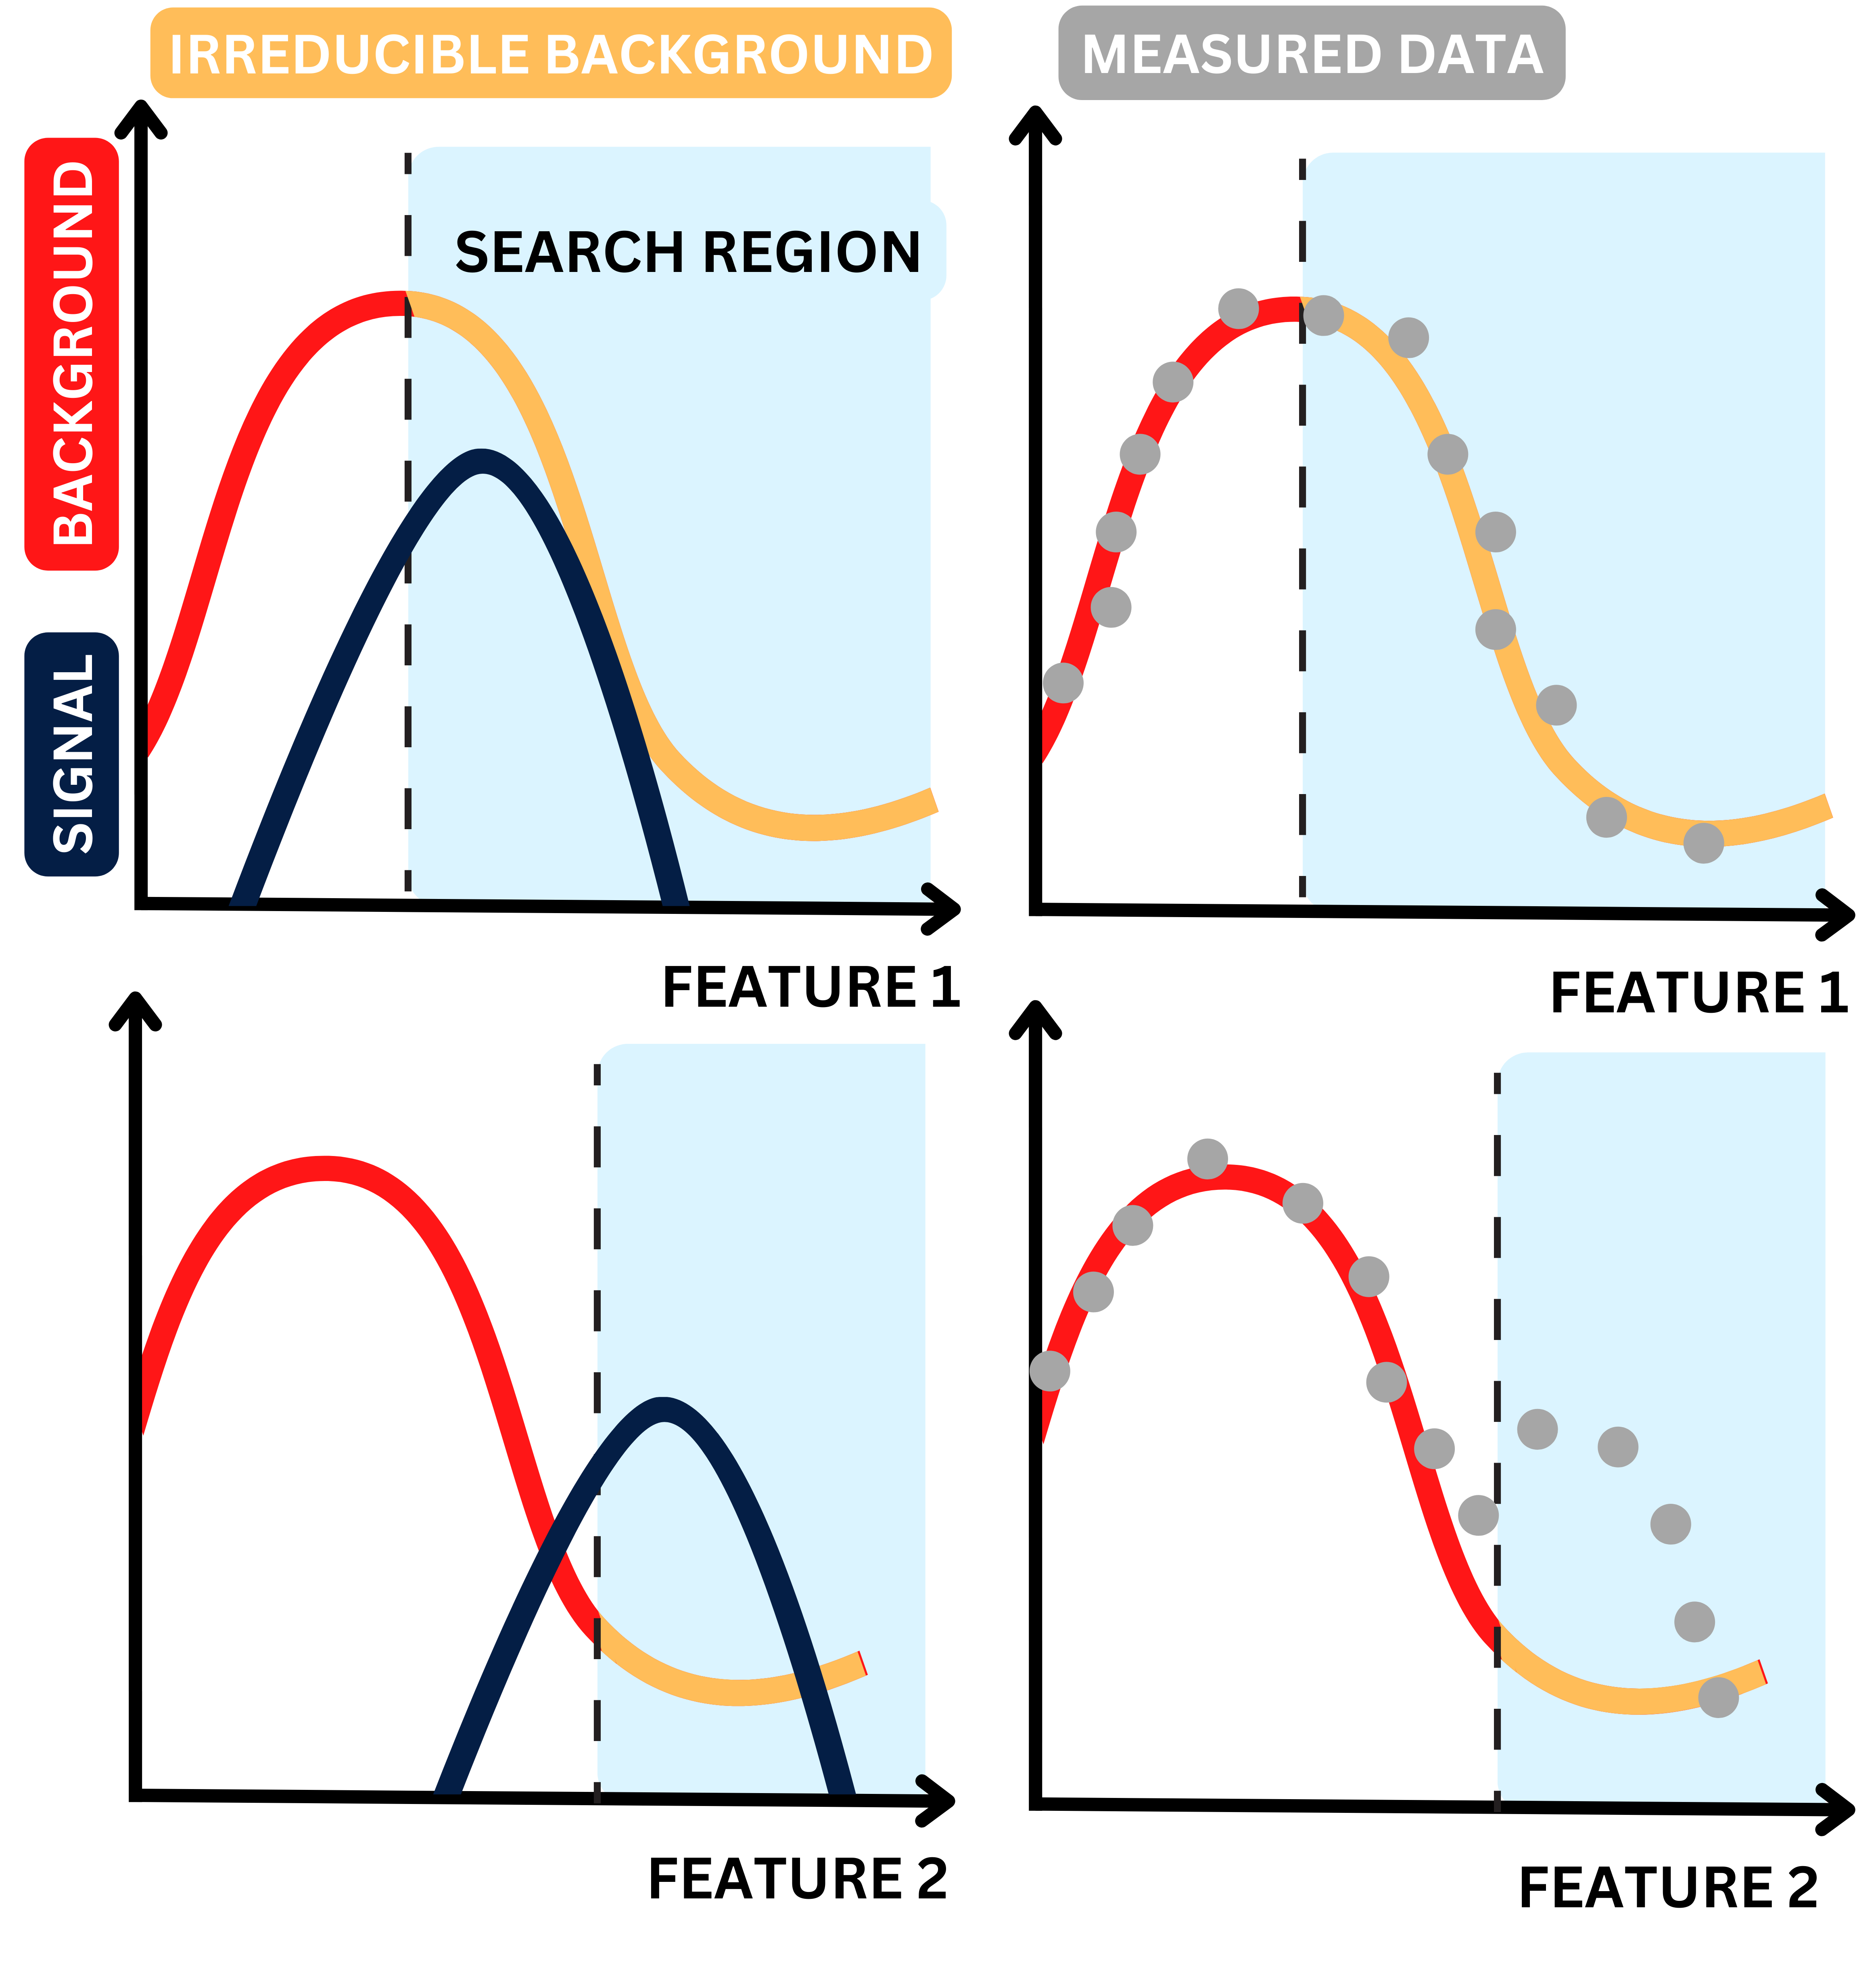
\includegraphics[width = 0.65\textwidth]{figures/DataComp.png}
% \end{frame}
% \begin{frame}{The search}
%     \begin{itemize}
%         \item Study application of supervised learning as it searches for SUSY signal 
%         \begin{itemize}
%             \item Chargino-neutralino production
%             \item 2 free parameters: masses of the chargino and neutralino
%         \end{itemize}
%         \item Measure sensitivity of an analysis 
%         \begin{itemize}
%             \item Expected significance
%             \item How many collisions do we expect to find in search region?
%         \end{itemize} 
%     \end{itemize}
%     % \vfill
%     \centering
%     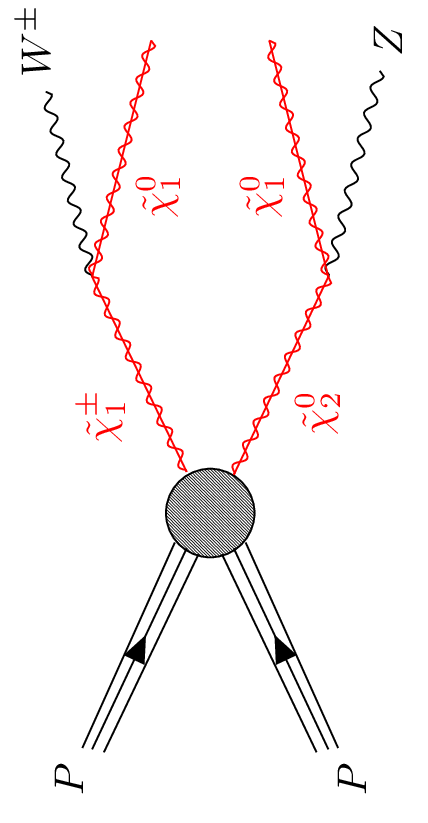
\includegraphics[width=0.3\textwidth, angle = -90]{figures/WZSignal.png}
% \end{frame}

% \begin{frame}{This thesis}
%     \vfill
%     \begin{center}
%         \emph{Shed some light on the application of supervised learning in HEP by 
%         experimenting and studying a set of ML methods as they search for a set of SUSY signals}
%     \end{center}
   
%     % \vspace{2cm}
%     % \vfill
%     % \begin{enumerate}
%     %     \item Study individual attributes of a set of supervised methods 
%     %     \item Compare expected sensitivity between methods on a subset of data
%     %     \item Attempt to increase sensitivity via feature reduction (PCA)
%     %     \item Compare the expected limits achieved by best performing methods 
%     %           to previous ATLAS analysis
%     % \end{enumerate}
%     \centering
% \end{frame}

\section{The Implementation}
\begin{frame}{The Implementation}
    \tableofcontents[currentsection]
\end{frame}

\begin{frame}{The SUSY signal}
    \begin{textblock}{0.4}(-0.02, 0.2)
        \begin{itemize}
            \item Chargino-neutralino production
            \item Free parameters $\rightarrow$ masses 
            \item Nr-of-Events(Mass)
        \end{itemize}
    \end{textblock}
    \begin{textblock}{.9}(0.4,0.175)
        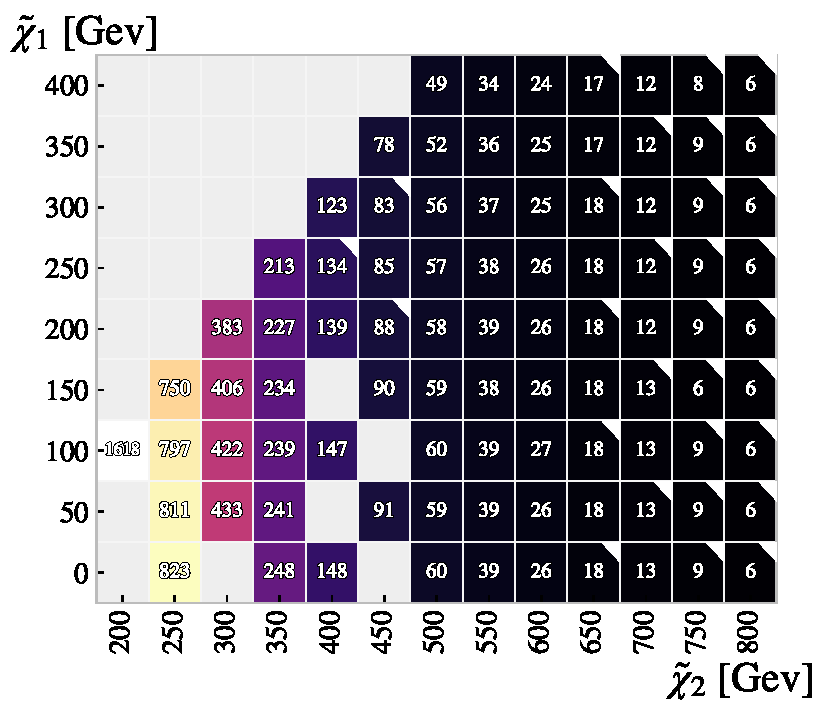
\includegraphics[width=0.65\textwidth]{figures/Signal/NrSignalEvents.pdf}
    \end{textblock}
\end{frame}

\begin{frame}{A summary of the applied methods}
    \begin{itemize}

    \item \emph{Three} neural network variants
    \begin{itemize}
        \item Ordinary dense neural network
        \item Ensemble networks utilizing Local-Winner-Takes-All (LWTA) layers
        \item Parameterized neural networks (PNN)
    \end{itemize}

    \item \emph{One} boosted decision tree method

    \end{itemize}

    \begin{textblock}{1}(0.,0.555)
        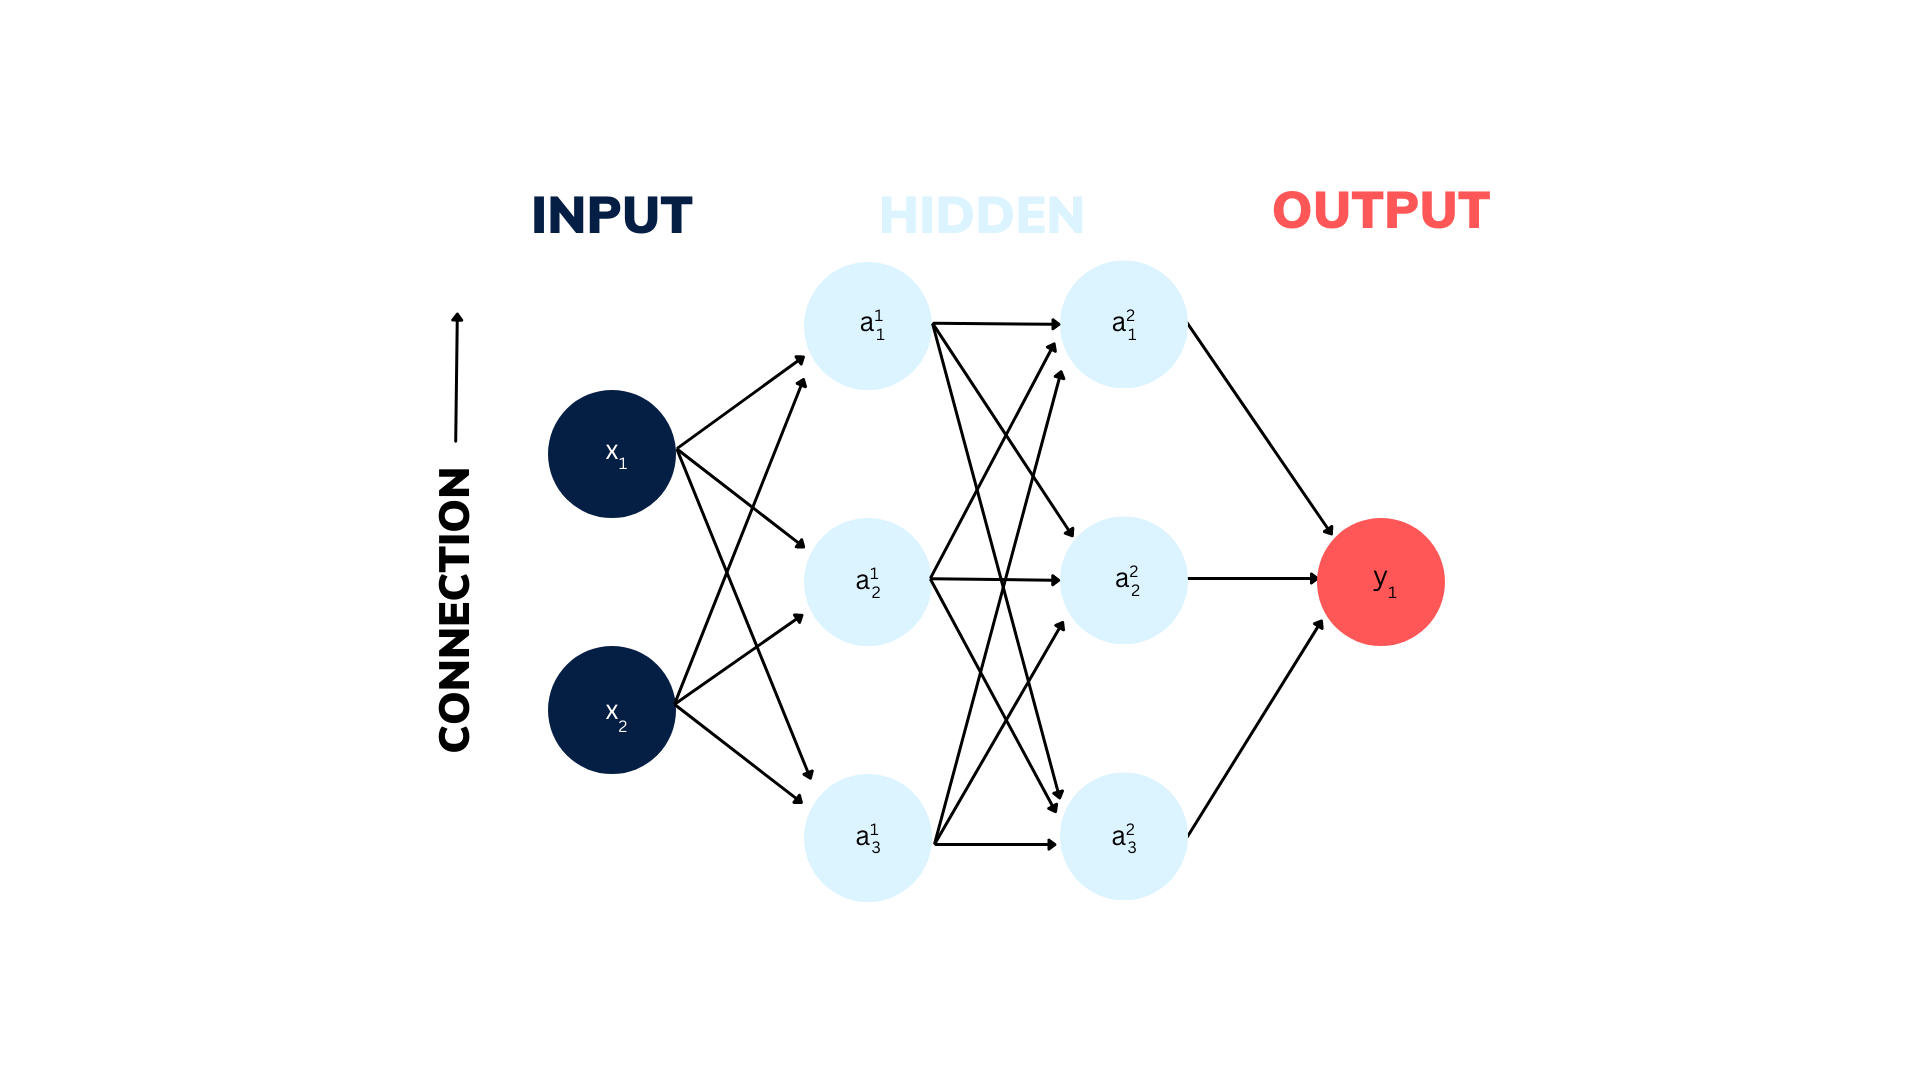
\includegraphics[width=0.525\textwidth]{figures/Input_labels.png}
    \end{textblock}
    \begin{textblock}{1}(.5,0.58)
        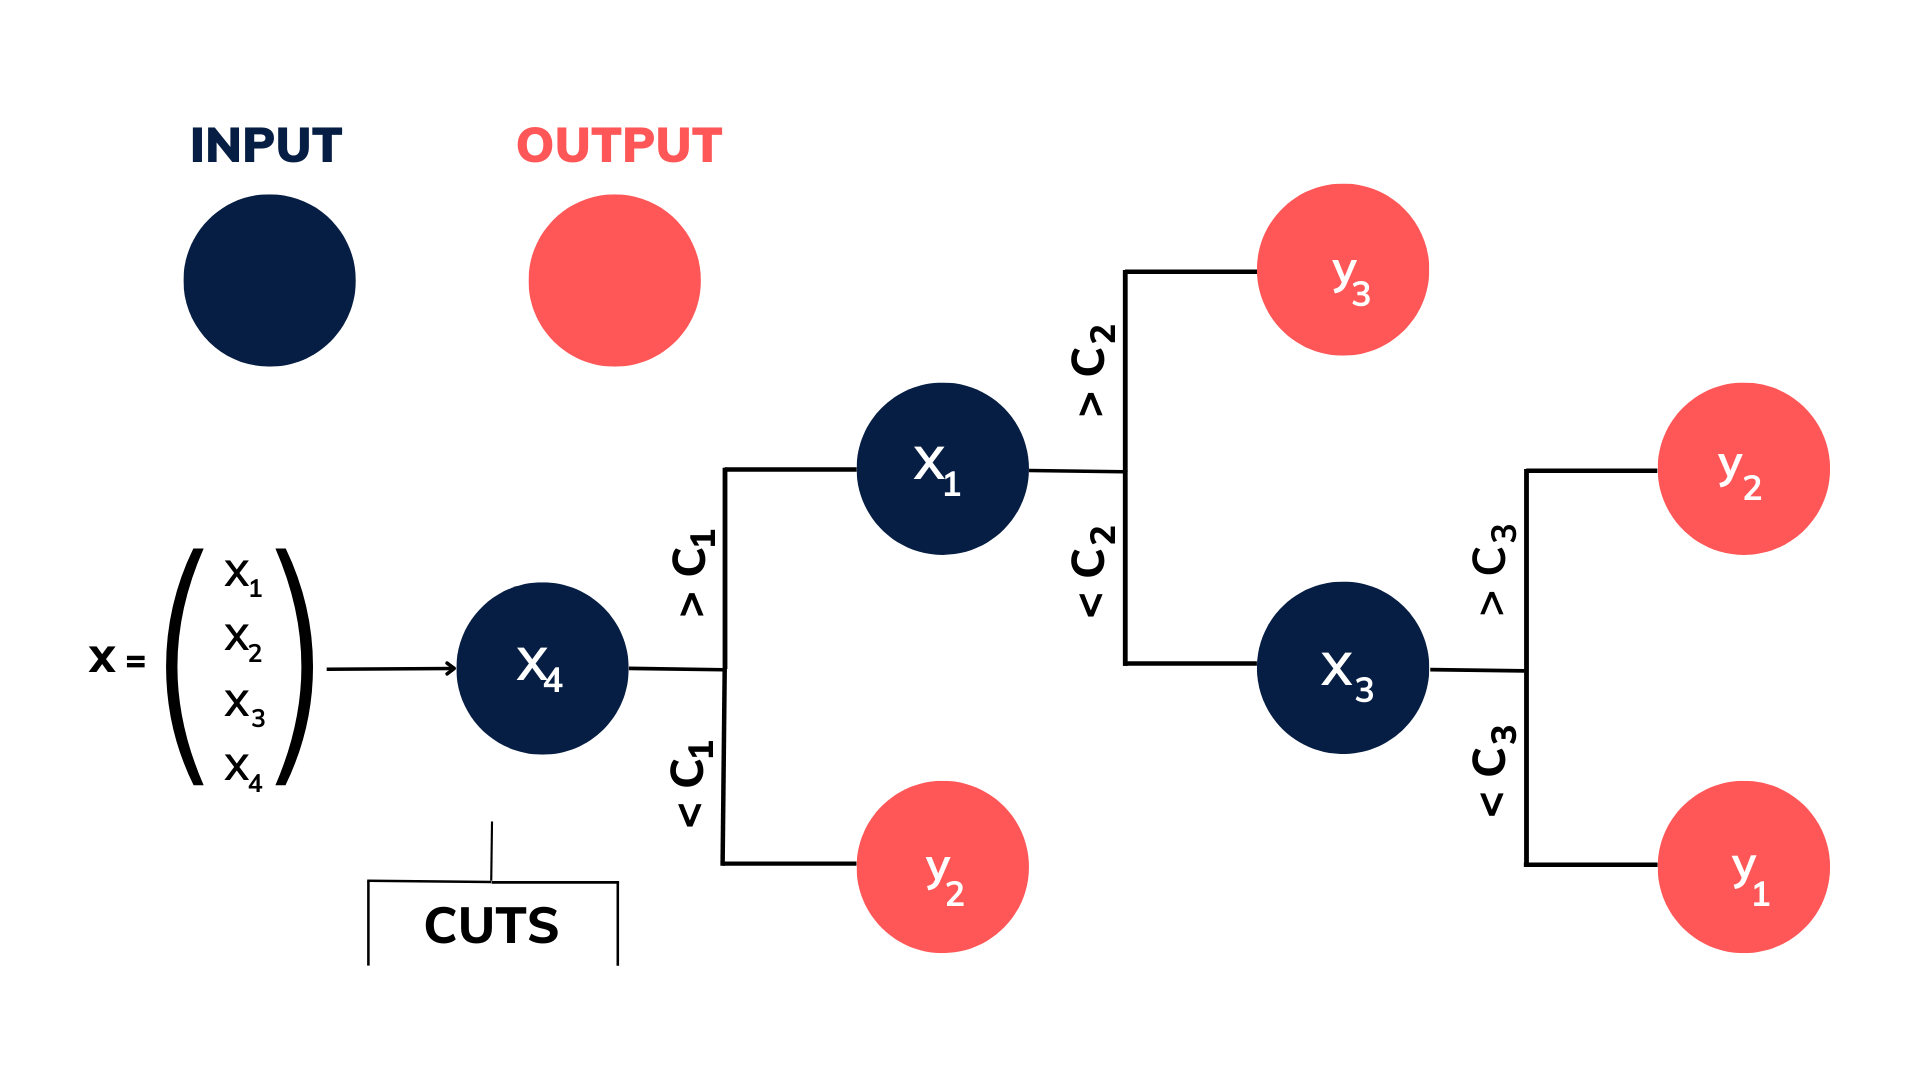
\includegraphics[width=0.435\textwidth]{figures/DT.png}
    \end{textblock}
\end{frame}

\begin{frame}{Training strategy}
    \begin{itemize}
        \item Objective
        \begin{itemize}
            \item Background $\rightarrow$ 0 
            \item Signal $\rightarrow$ 1
        \end{itemize}
        \item $80\%$ training and $20\%$ validation 
        \item Early stopping criteria
        \begin{itemize}
            \item Train as long as performance on validation set improves 
            \item Patience 10 epochs
            \item Reset weights to best epoch
        \end{itemize}
    \end{itemize}
\end{frame}



\section{Methods $\&$ Results}
\begin{frame}{Methods $\&$ Results}
    \tableofcontents[currentsection]
\end{frame}


% \begin{frame}{Boosted decision trees - XGBoost}
%     \begin{textblock}{1}(0.375, 0.15)
%         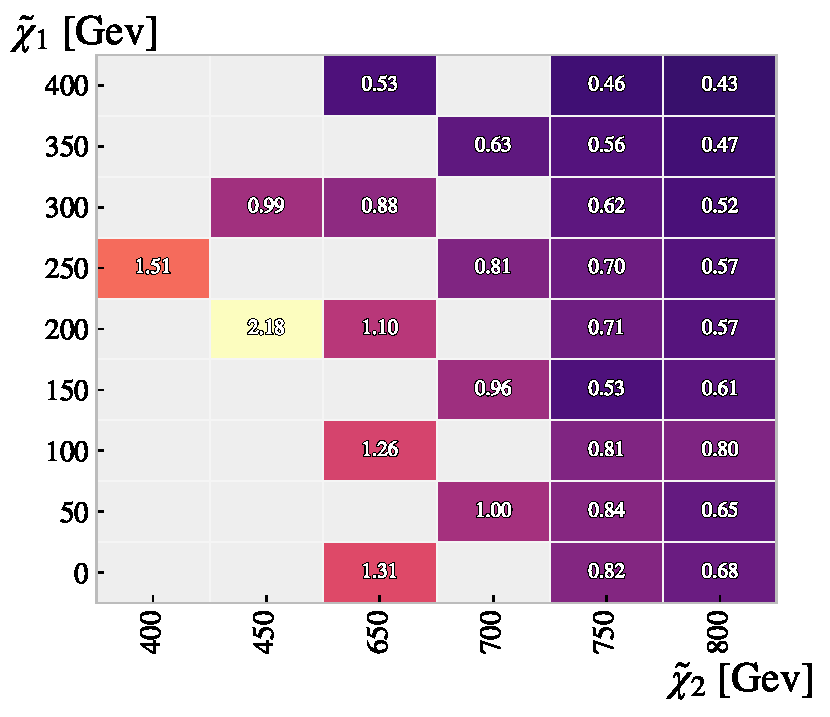
\includegraphics[width=0.6\textwidth]{figures/grids/XGBGridSig.pdf}    
%     \end{textblock}
%     \begin{textblock}{0.4}(-0.01, 0.2)
%         \begin{itemize}
%             \item Used as benchmark
%             \item Displayed better performance on lower masses  
%         \end{itemize}
%     \end{textblock}
% \end{frame}

% \begin{frame}{Sensitivity grid}
%     \vfill
%     \begin{center}
%         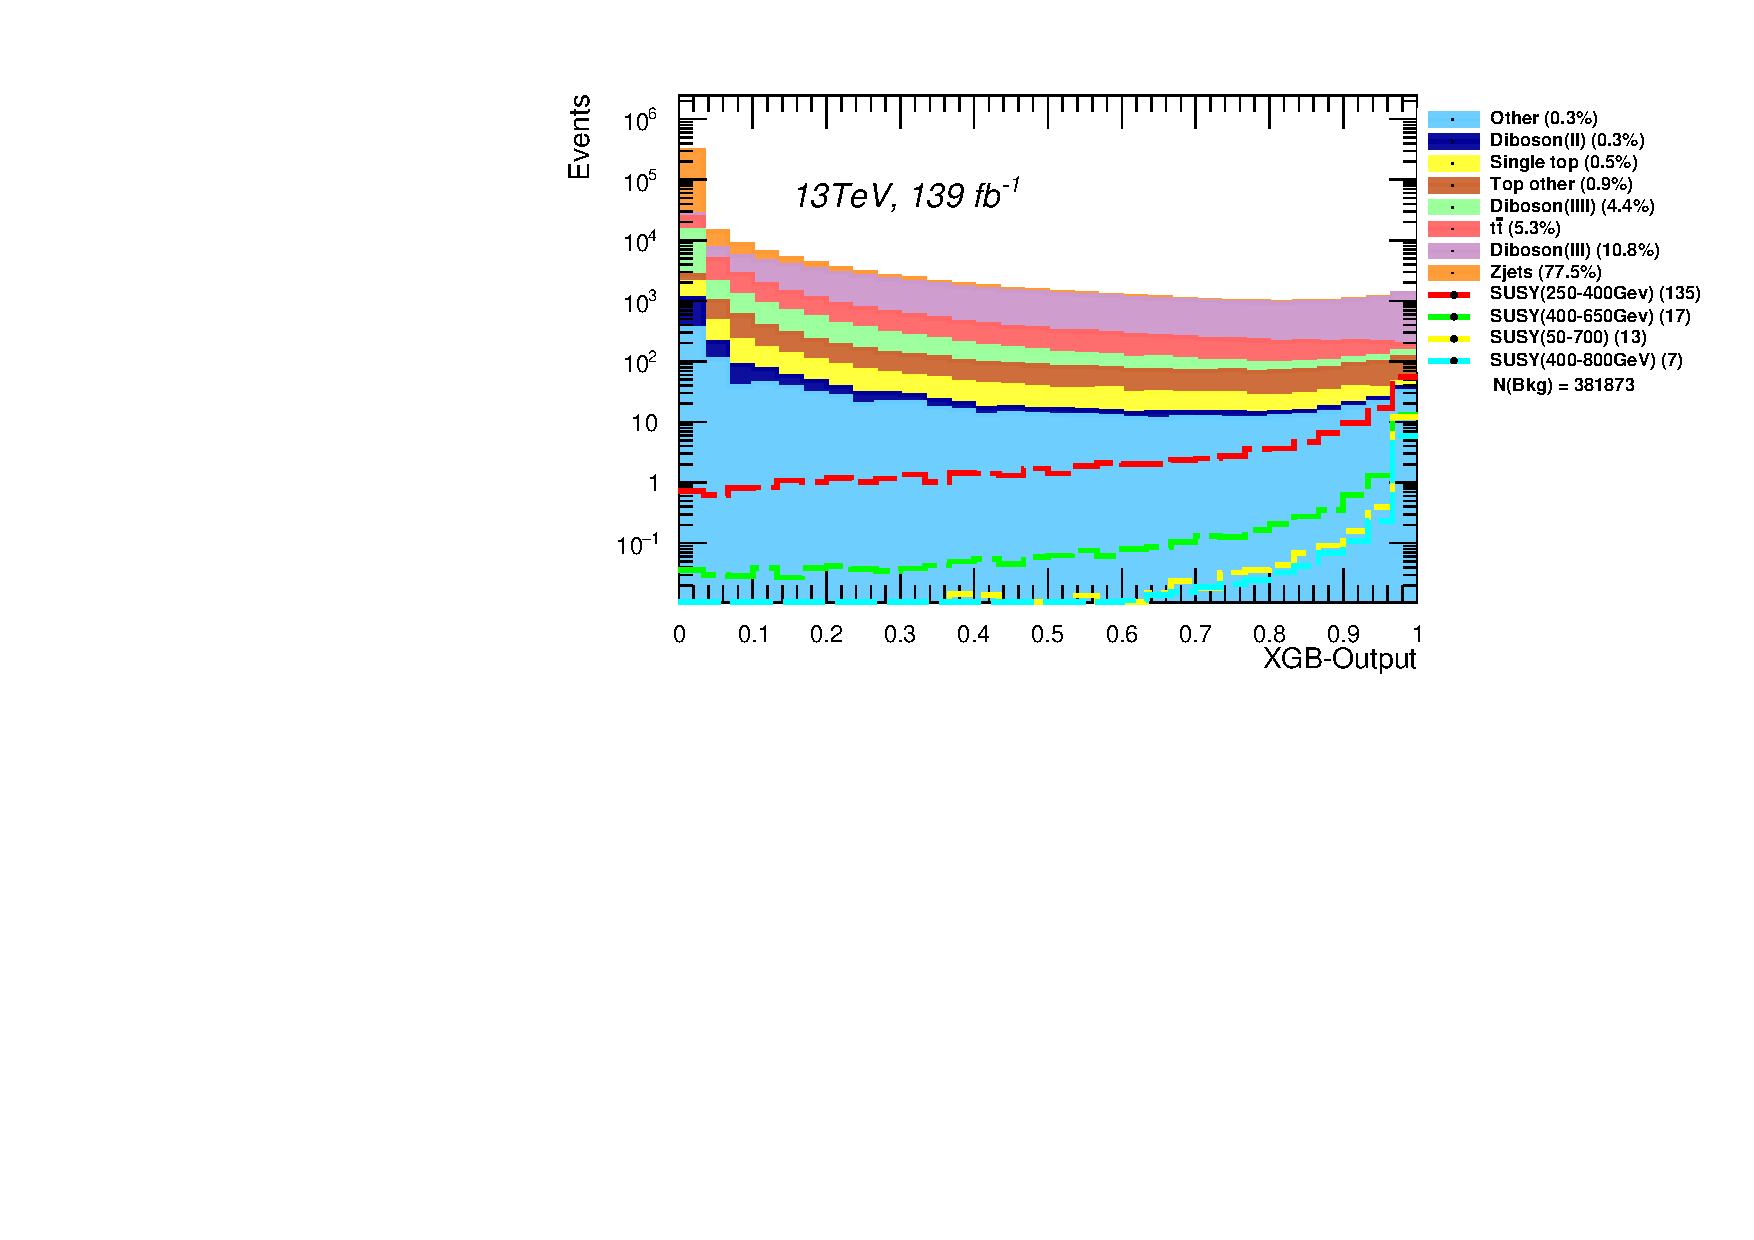
\includegraphics[width = 0.475\textwidth]{figures/dists/xgbDist.pdf}
%         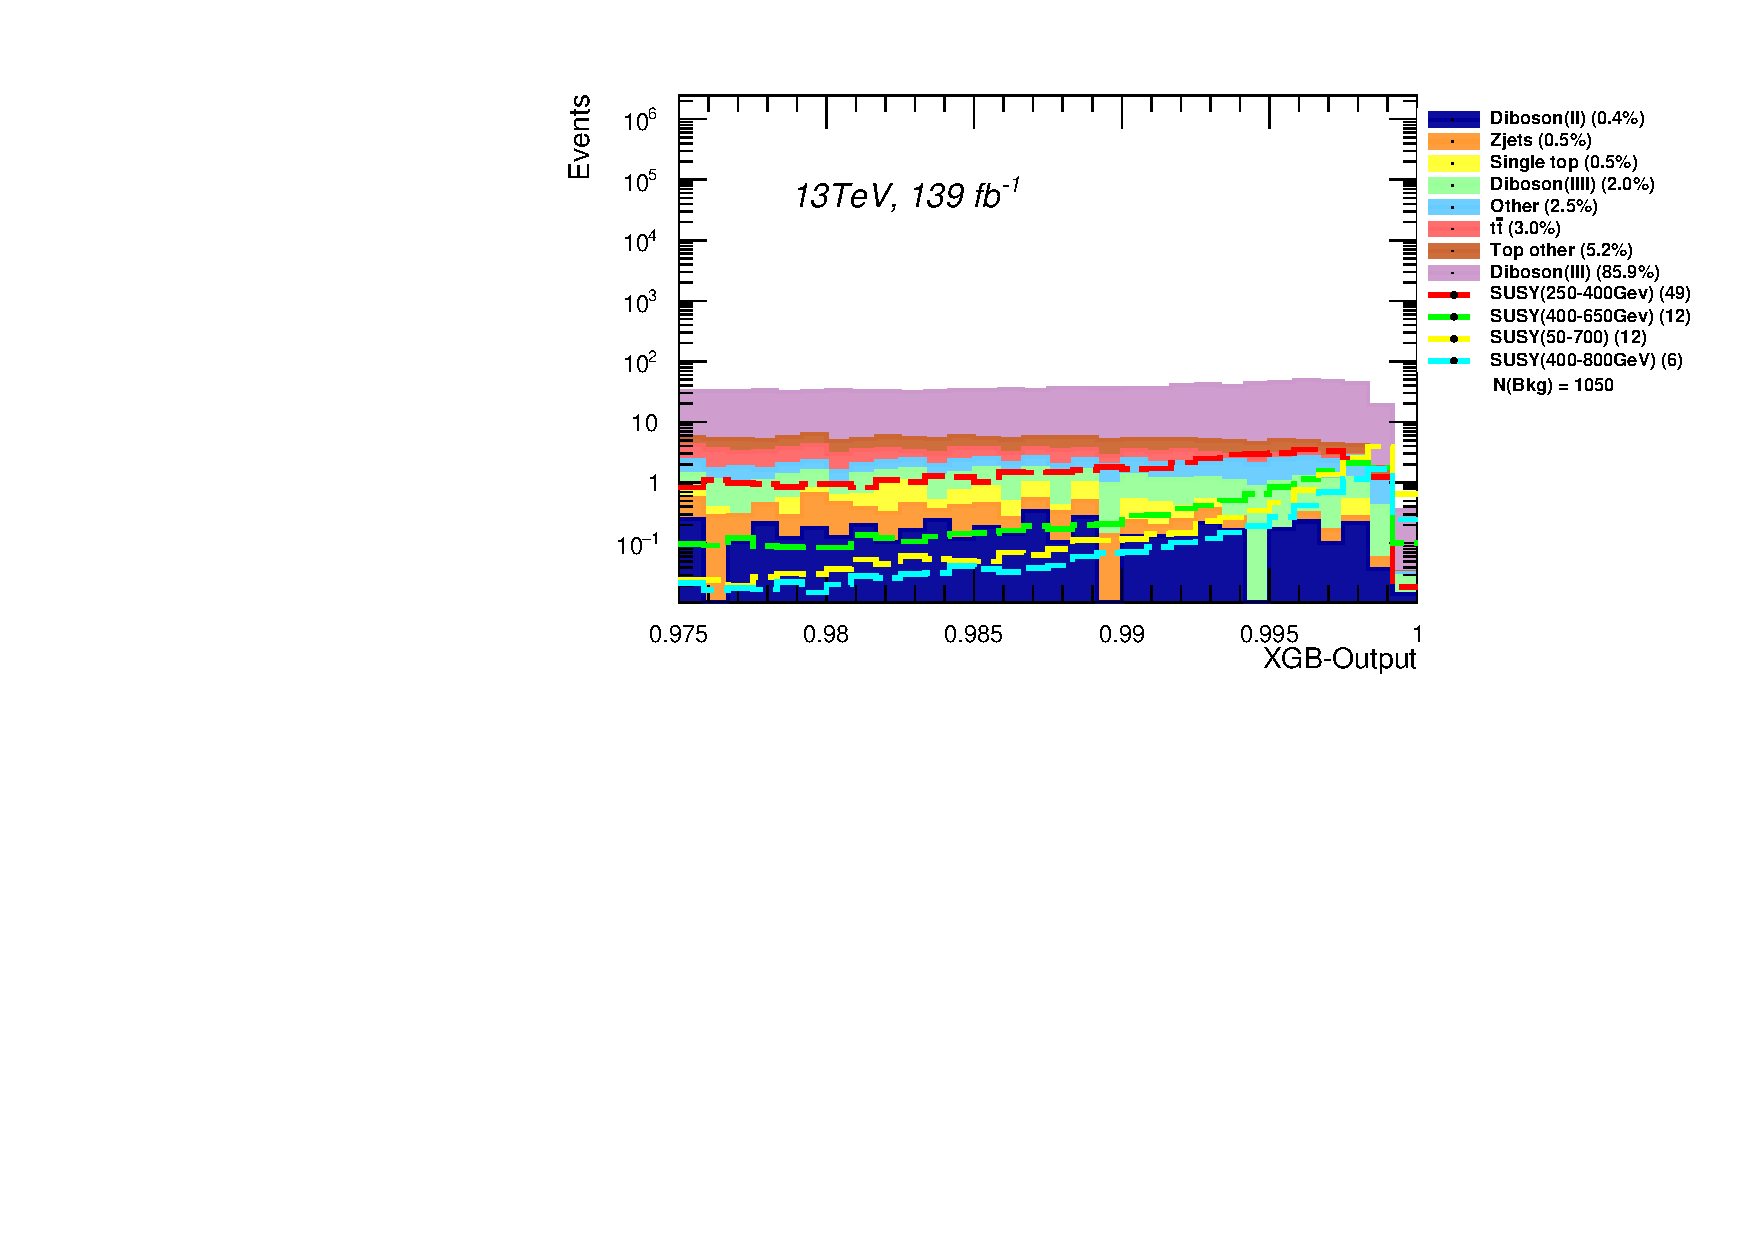
\includegraphics[width = 0.475\textwidth]{figures/dists/xgbDist_C7.pdf}
%     \end{center}
% \end{frame}

\begin{frame}{Ordinary dense neural network}
    \vfill
    \centering
    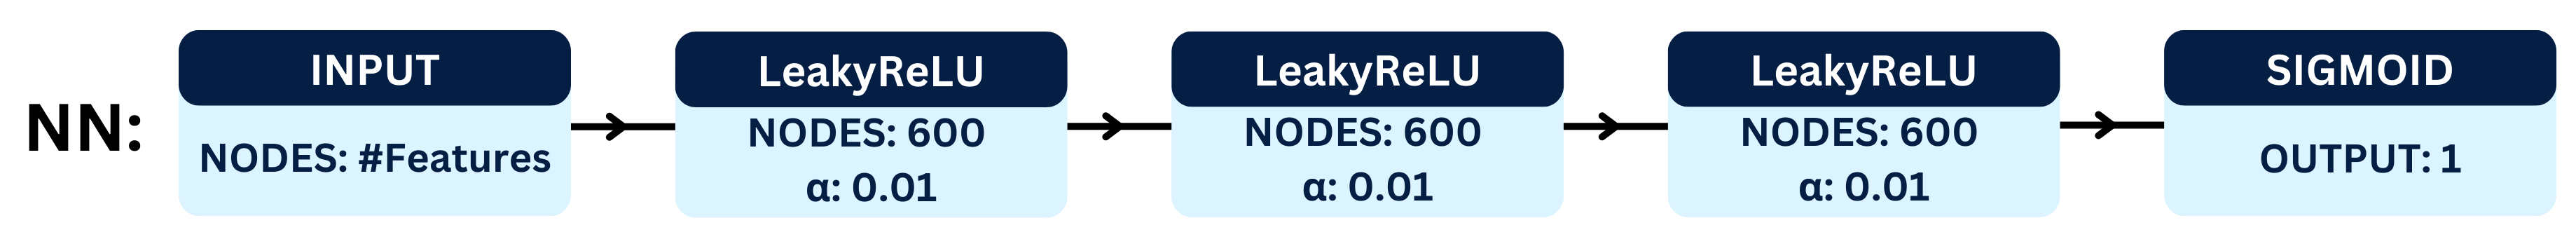
\includegraphics[width = 0.98\textwidth]{figures/NN.png}
\end{frame}
\begin{frame}{Compare one-mass approach to several-masses approach}
    \vfill
    \begin{center}
        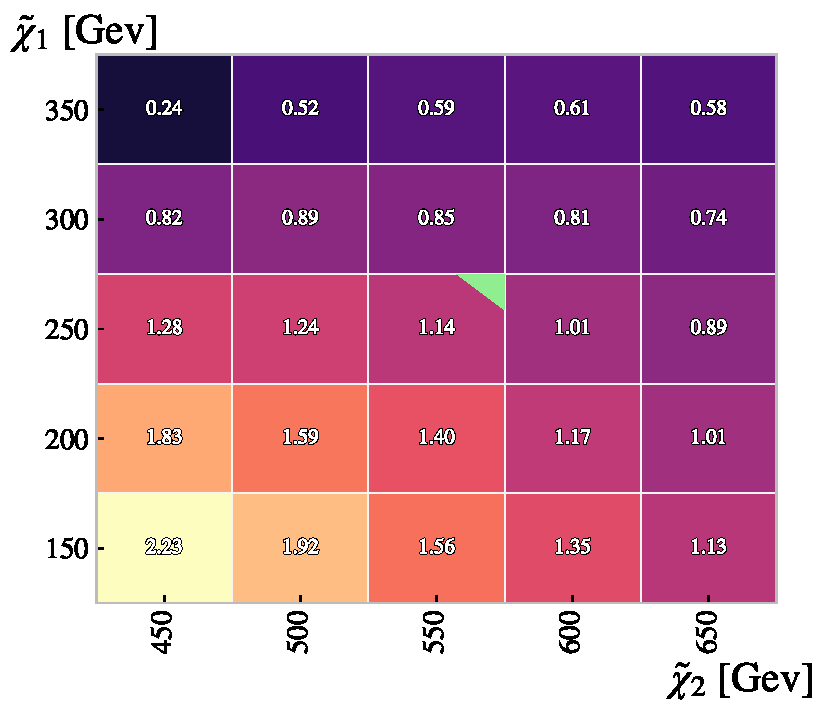
\includegraphics[width = 0.475\textwidth]{figures/grids/NN_OneMass_InterpolationGridSig.pdf}
        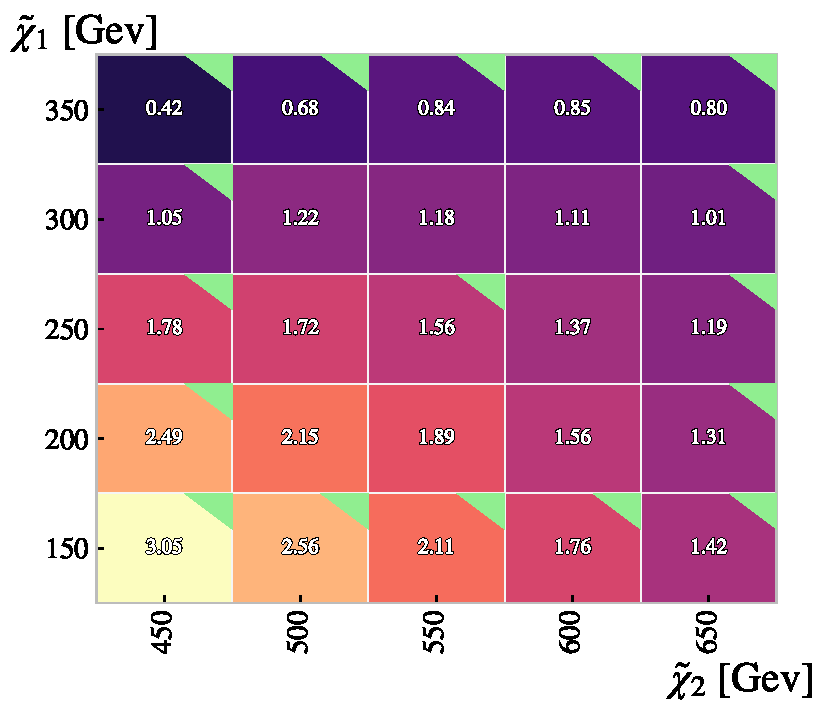
\includegraphics[width = 0.475\textwidth]{figures/grids/NN_InterpolationGridSig.pdf}
    \end{center}
\end{frame}


\begin{frame}{Parameterized neural network}
    \begin{itemize}
        \item Long-term memory
        \item PNN $\rightarrow$ signal includes mass parameter in feature set
        \item Background assigned
        parameters randomly
        using same distribution
        as signal
        \item Motivation
        \begin{itemize}
            \item Network will \\
            associate parameters\\
            with trends in the \\
            data
        \end{itemize}
        \begin{textblock}{0.8}(0.45, 0.35)
            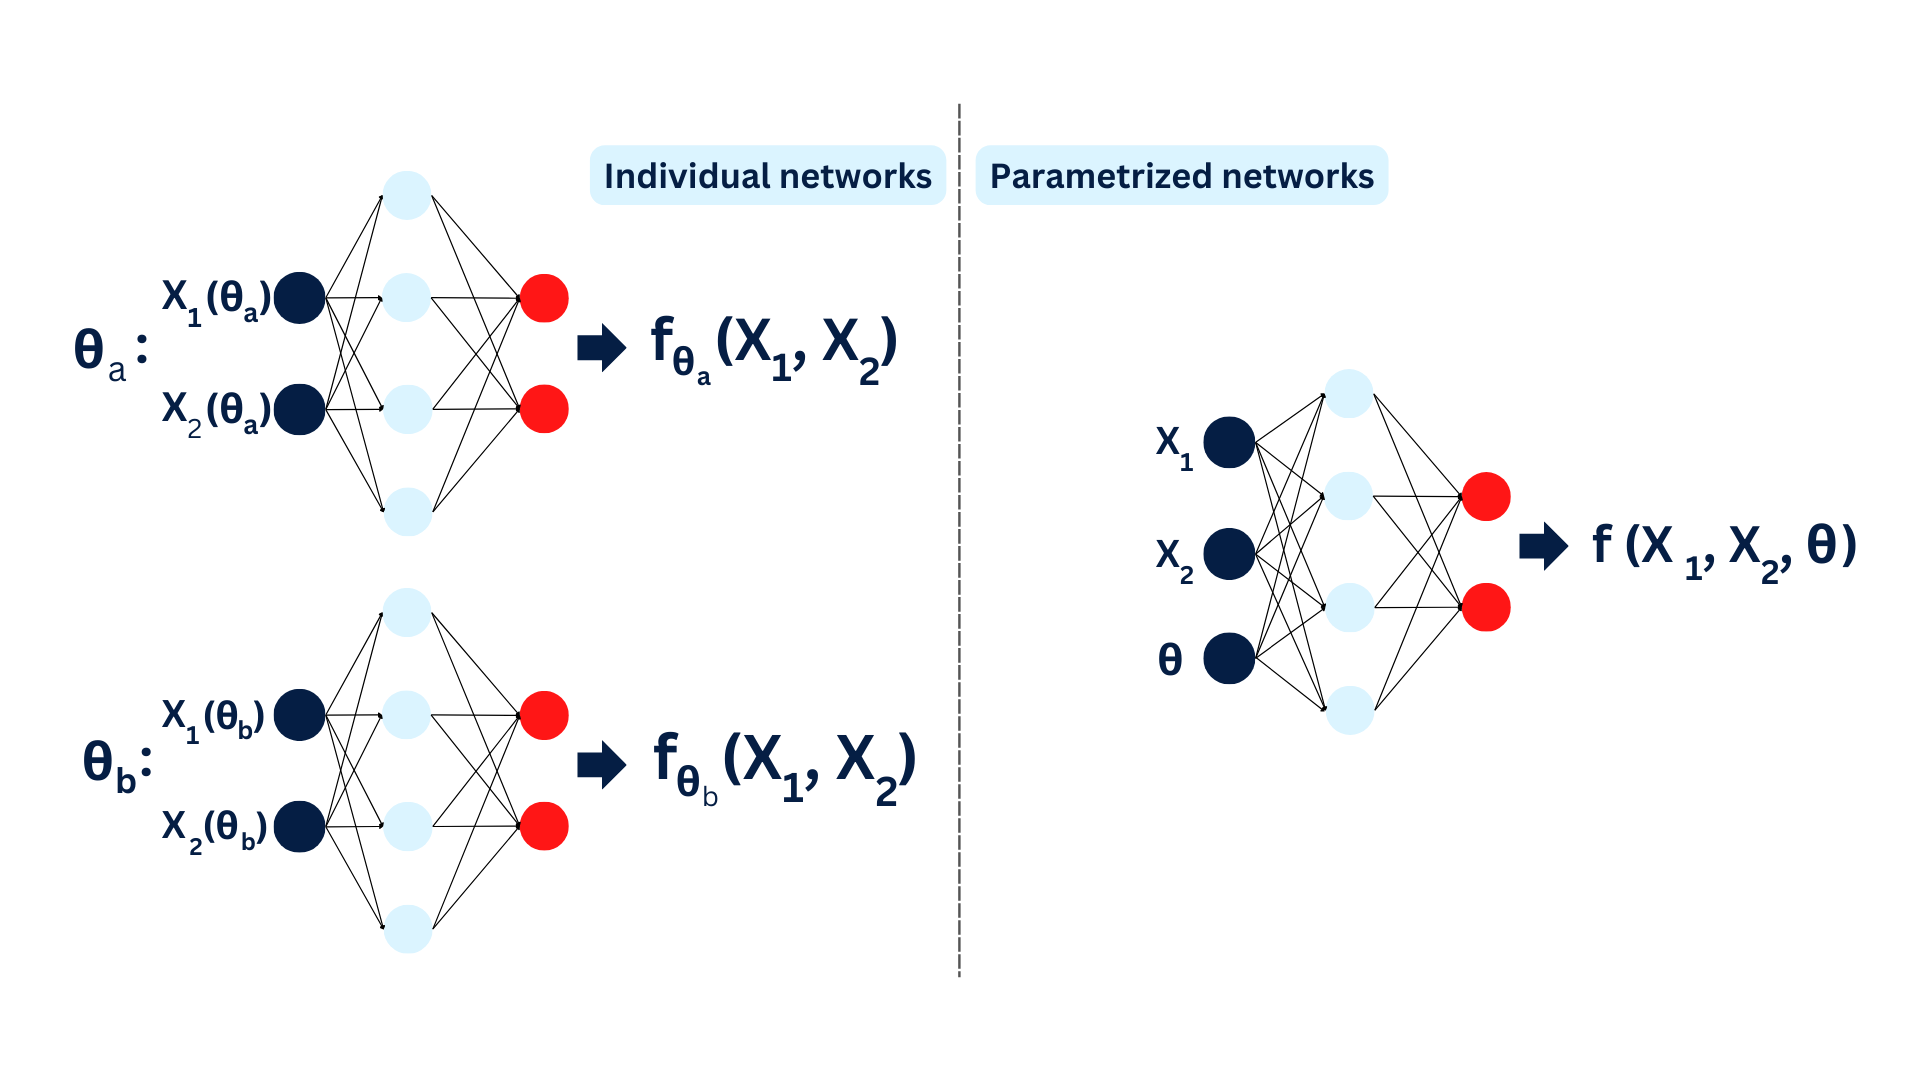
\includegraphics[width = 0.7\textwidth]{figures/PNN.png}
        \end{textblock}
    \end{itemize}
\end{frame}
% \begin{frame}{PNN architecture}
%     \vfill
%     
\includegraphics[width = 0.98\textwidth]{figures/PNNArch.png}
% \end{frame}
% \begin{frame}{Study the effect of the parameters in the PNN}
%     \begin{itemize}
%         \item Test: Manually assign all the events the same parameters thereby assigning
%         most of the signal the wrong parameters
%         \item Hypothesis: PNN performs better when events are assigned correct
%         parameters 
%         \item First test: $\{50,250\}_{GeV}$
%         \item Second test: $\{200,300\}_{GeV}$
%     \end{itemize}
%     \begin{table}
%         \tiny
%         \centering
%         $
%         \begin{array}{cccccc}
%             \hline \text { \diagbox{\textbf{Parameters}}{\textbf{Channel}} }  & \text {$\{50,250\}_{GeV}$} & \text {$\{100,200\}_{GeV}$} & \text {$\{150,300\}_{GeV}$} & \text {$\{200,300\}_{GeV}$} & \text {$(Background)$} \\
%             \hline \text {$(50,250)$}   & \text { $\bf{80.8}\%$ } & \text { $45.8\%$ } & \text { $\bf{77.5}\%$ } & \text { $50.1\%$ } & \text { $2.4\%$ }  \\
%             \text {$(200,300)$}   & \text { $77.3\%$ } & \text { $\bf{54.6}\%$ } & \text { $76.3\%$ } & \text { $\bf{59.0}\%$ } & \text { $\bf{2.7}\%$ }\\
%             \hline
%         \end{array}
%         $
%     \end{table}
% \end{frame}

\begin{frame}{Ensemble methods - LWTA}
    \begin{itemize}
        \item Local-Winnder-Takes-All
        \item Competing nodes - Units
        \item Encode information in pattern specific pathways
    \end{itemize}    
    \centering
    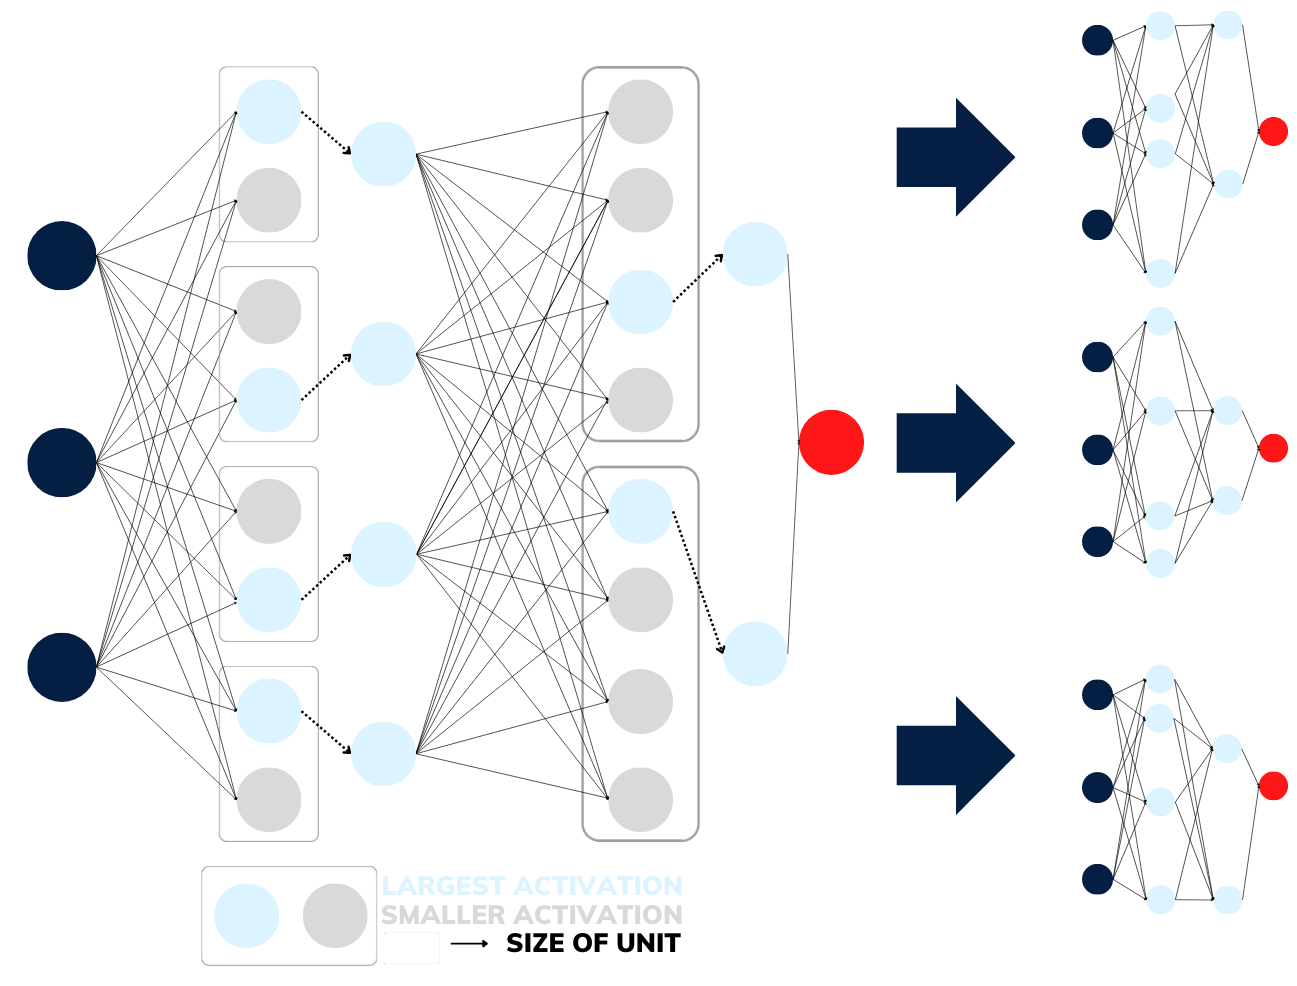
\includegraphics[width = 0.5\textwidth]{figures/Max_out}
\end{frame}

\begin{frame}{Channel-Out, SCO and Maxout}
    \vspace{0.5cm}
    \center
        \begin{table}
            $
            \begin{array}{ccc}
                \hline \text { Layer } & \text { Separate weights} & \text { Static units }\\
                \hline\hline\text{Channel-Out} & \checkmark &  \checkmark  \\
                \text { SCO } &  \checkmark &  $X$ \\
                \text{ Maxout } &  $X$ &  \checkmark   \\
                \hline
            \end{array}
            $
        \end{table}
    \begin{textblock}{0.8}(0.1, 0.45)
        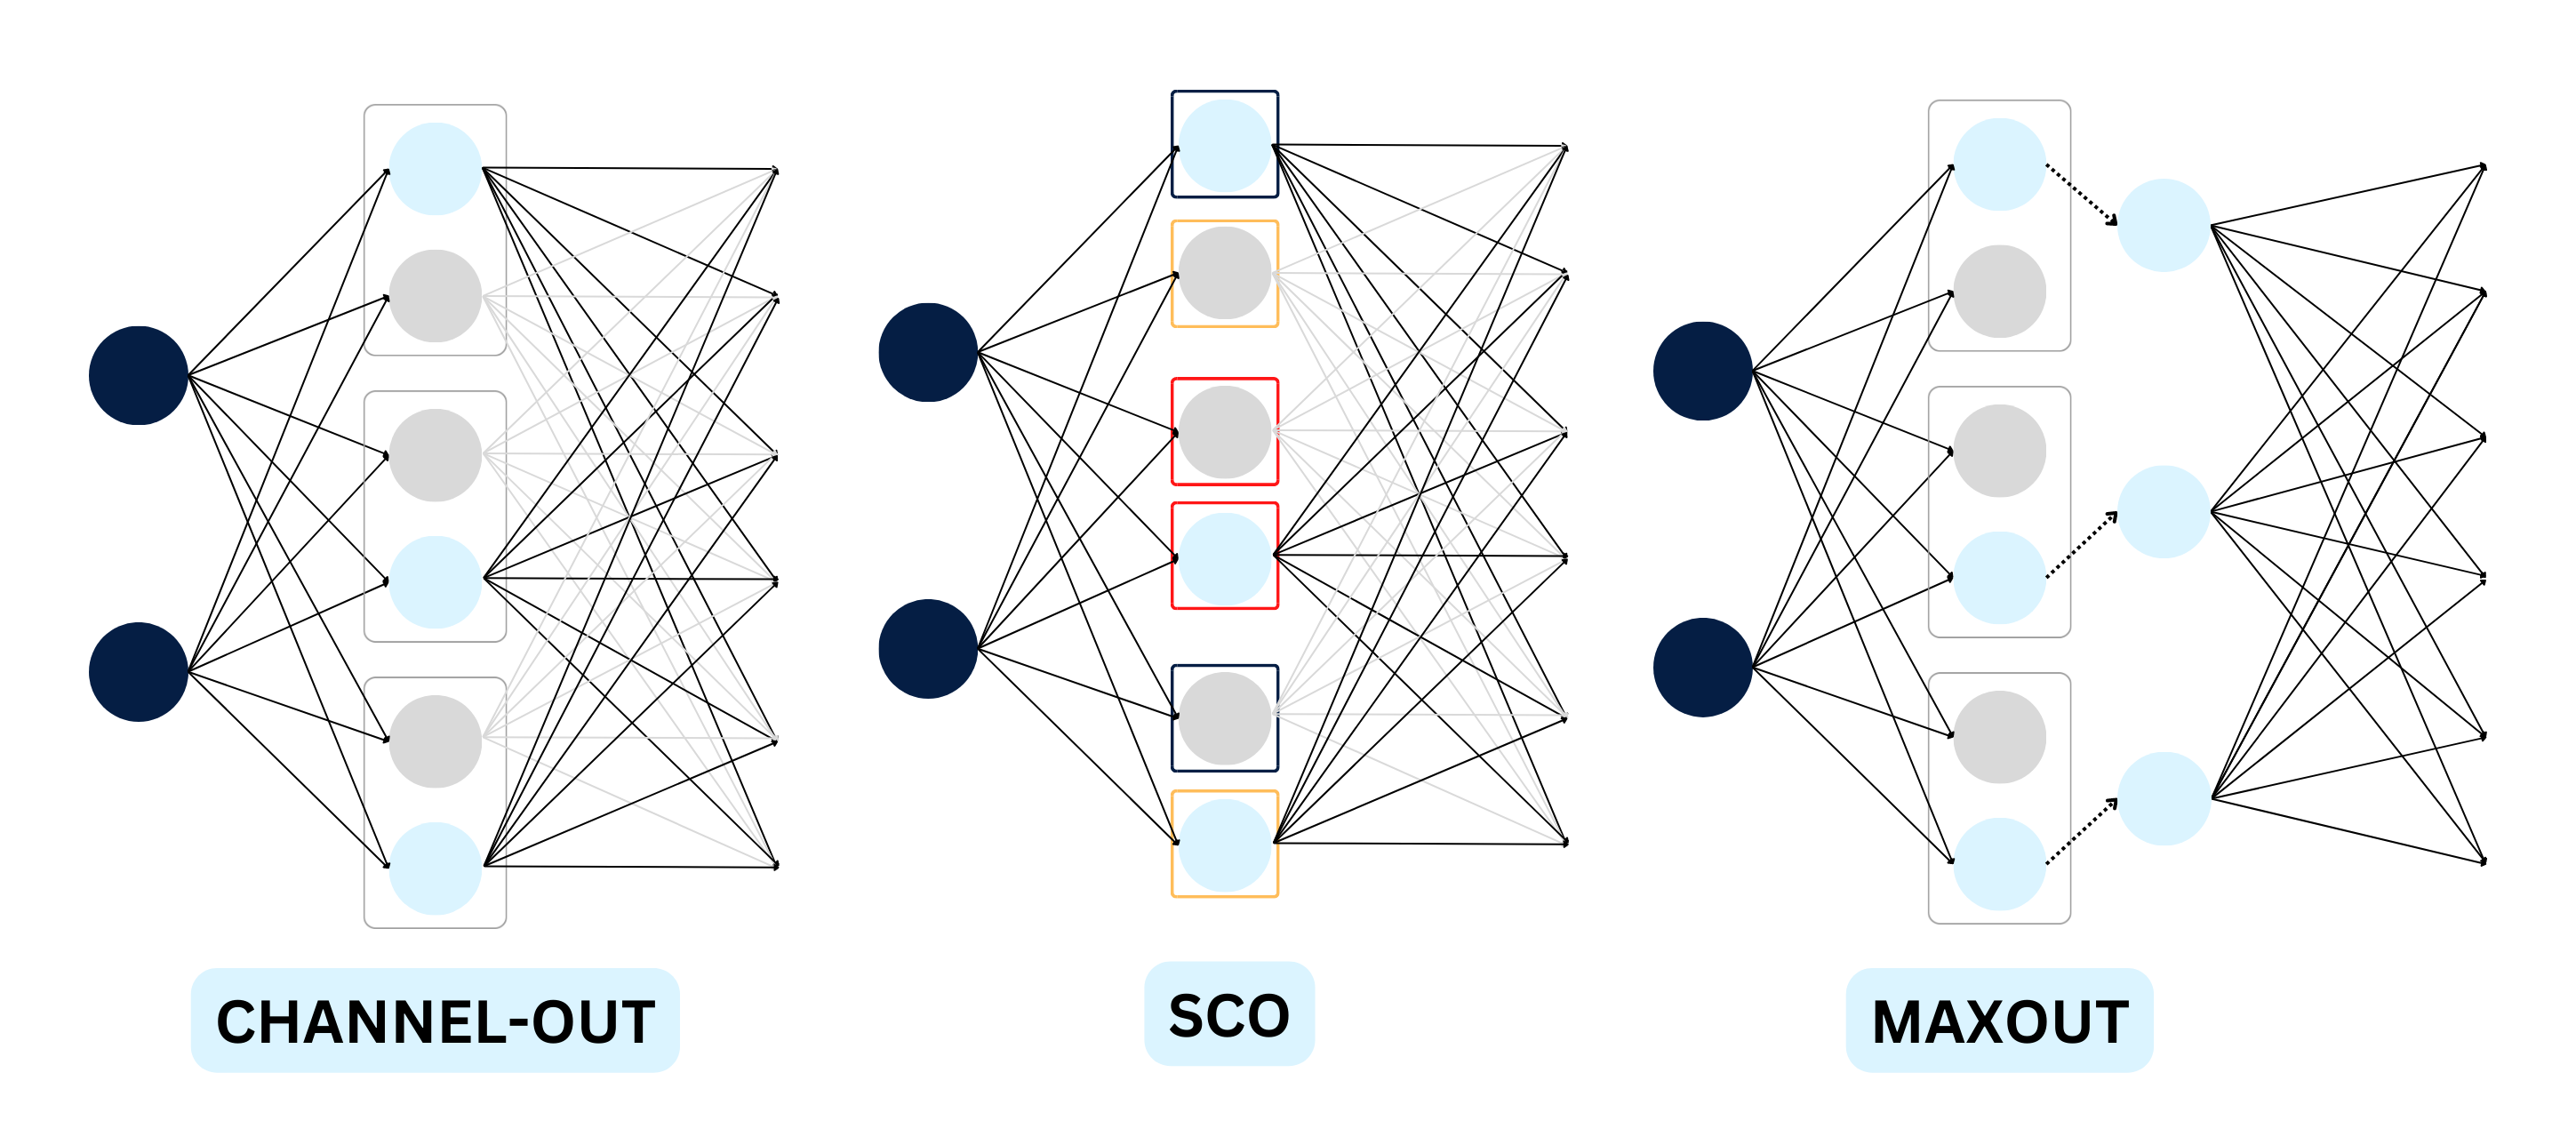
\includegraphics[width = \textwidth]{figures/EnsembleComp}
    \end{textblock}
\end{frame}

\begin{frame}{Visualization and study of sparse pathways}
    \begin{textblock}{0.8}(0.565, 0.15)
        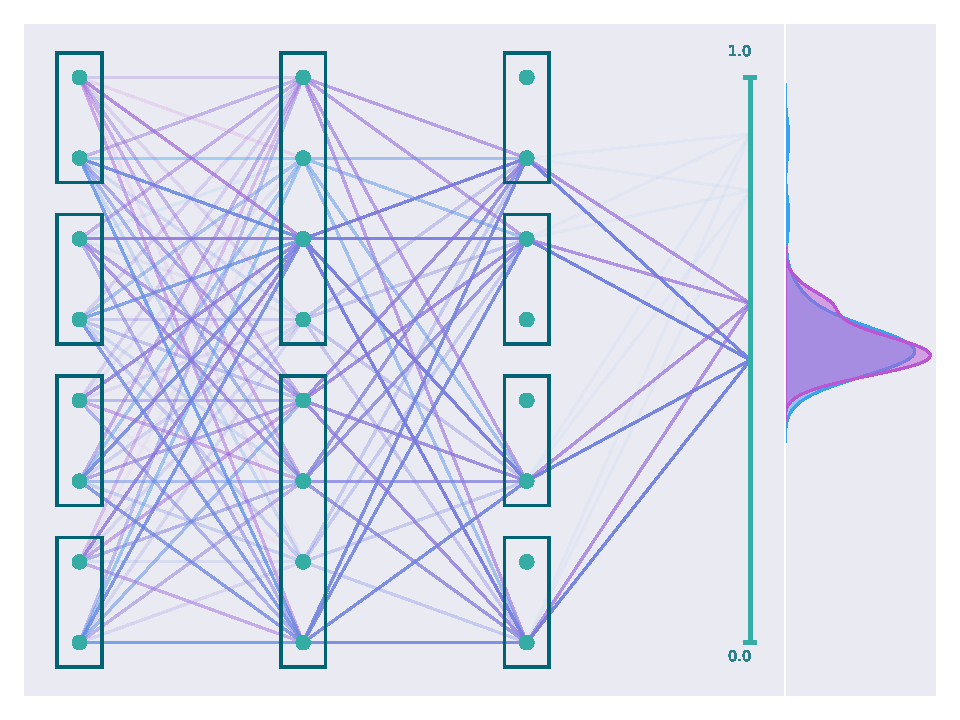
\includegraphics[width = 0.5\textwidth]{figures/NetworkVis/BeforeTraining.pdf}
        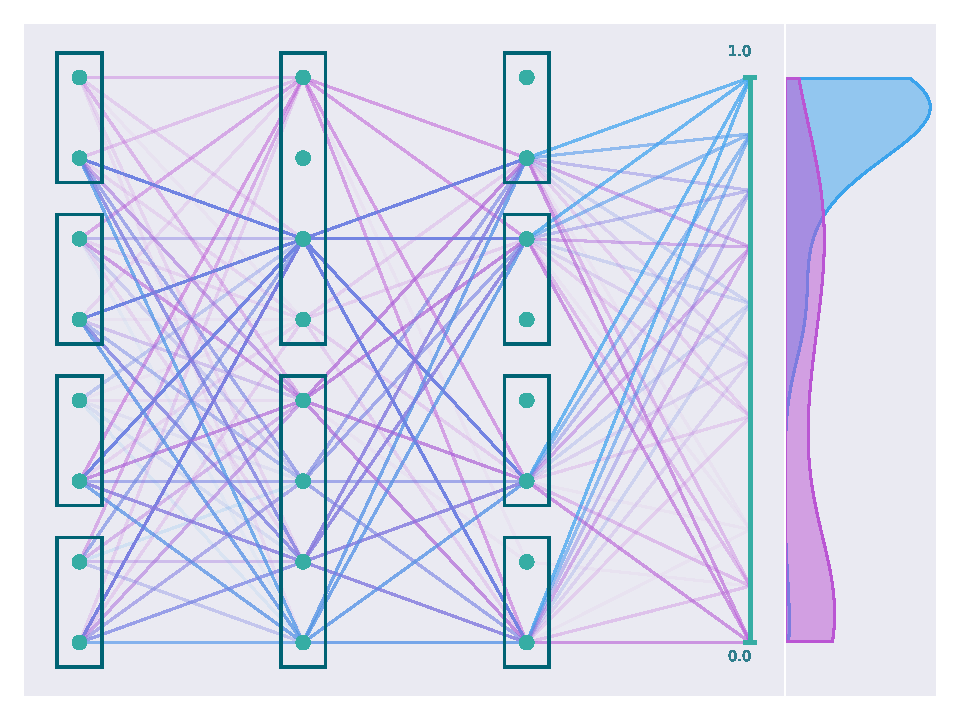
\includegraphics[width = 0.5\textwidth]{figures/NetworkVis/AfterTraining.pdf}
    \end{textblock}
    \begin{itemize}
        \item Visualize the activation and \\
        paths of randomly sampled \\
        events
        \item The bolder the line the more\\ 
        frequently the path is used.
        \item Color of lines 
        \begin{itemize}
            \item Pink: SM background
            \item Blue: SUSY signal
        \end{itemize}
    \end{itemize}
\end{frame}
\begin{frame}[noframenumbering]{Visualization and study of sparse pathways}
    \begin{textblock}{0.8}(0.565, 0.15)
        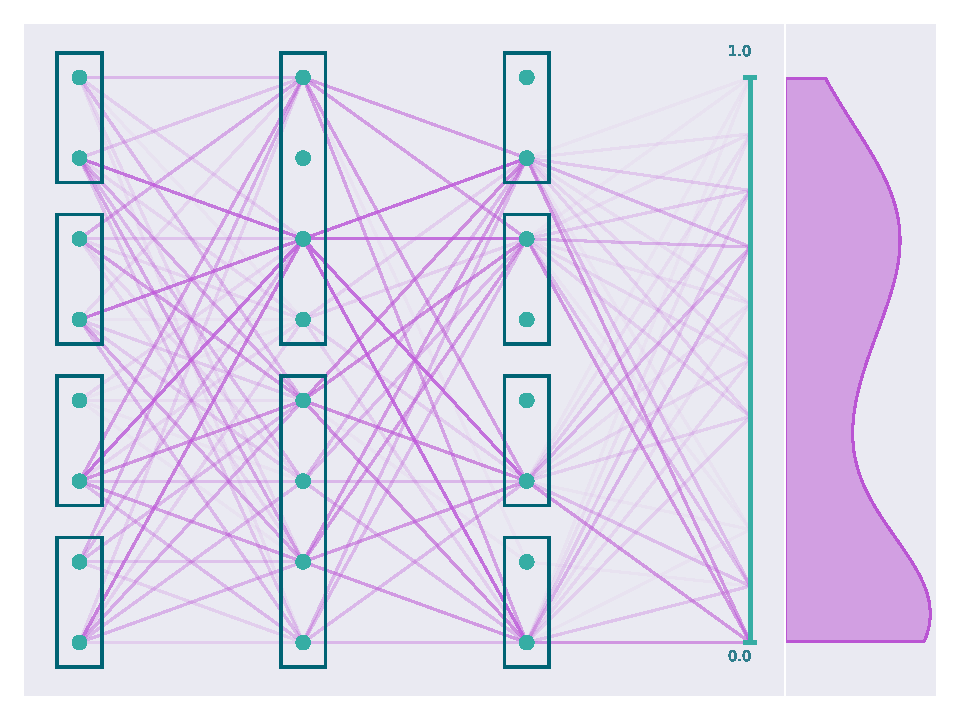
\includegraphics[width = 0.5\textwidth]{figures/NetworkVis/AfterTrainingBkg.pdf}
        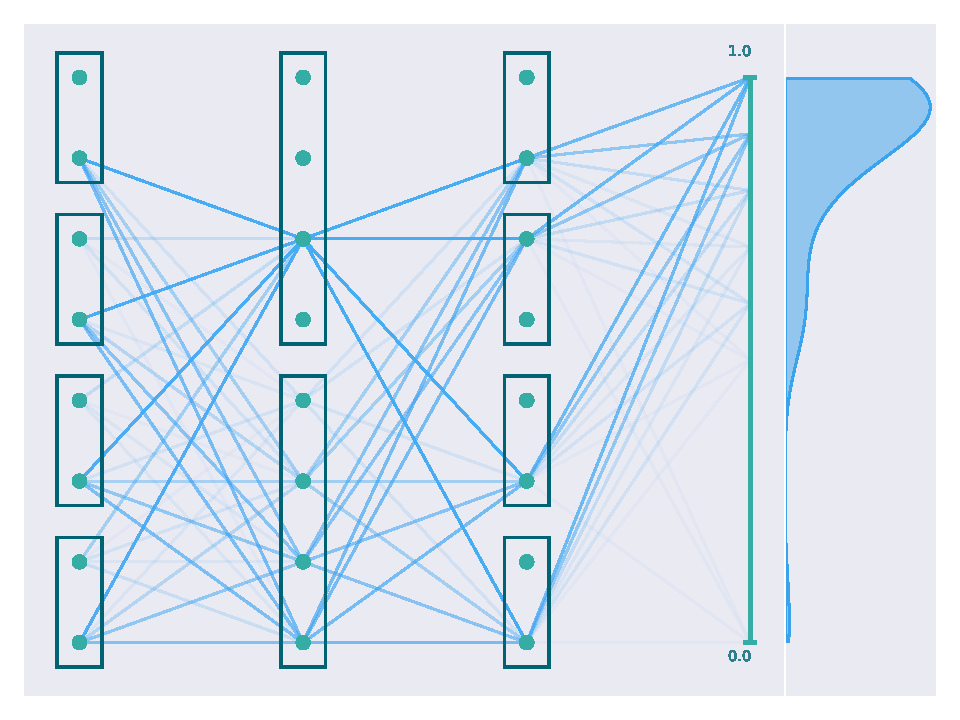
\includegraphics[width = 0.5\textwidth]{figures/NetworkVis/AfterTrainingSig.pdf}
    \end{textblock}
    \begin{itemize}
        \item Visualize the activation and \\
        paths of randomly sampled \\
        events
        \item The bolder the line the more\\ 
        frequently the path is used.
        \item Color of lines 
        \begin{itemize}
            \item Pink: SM background
            \item Blue: SUSY signal
        \end{itemize}
    \end{itemize}
\end{frame}



\begin{frame}{Comparing activation of Maxout with SCO}
    \begin{textblock}{0.8}(0.225, 0.8)
        {Maxout}
    \end{textblock}
    \begin{textblock}{0.8}(0.7, 0.8)
        {SCO}
    \end{textblock}
    \vfill
    \begin{center}
        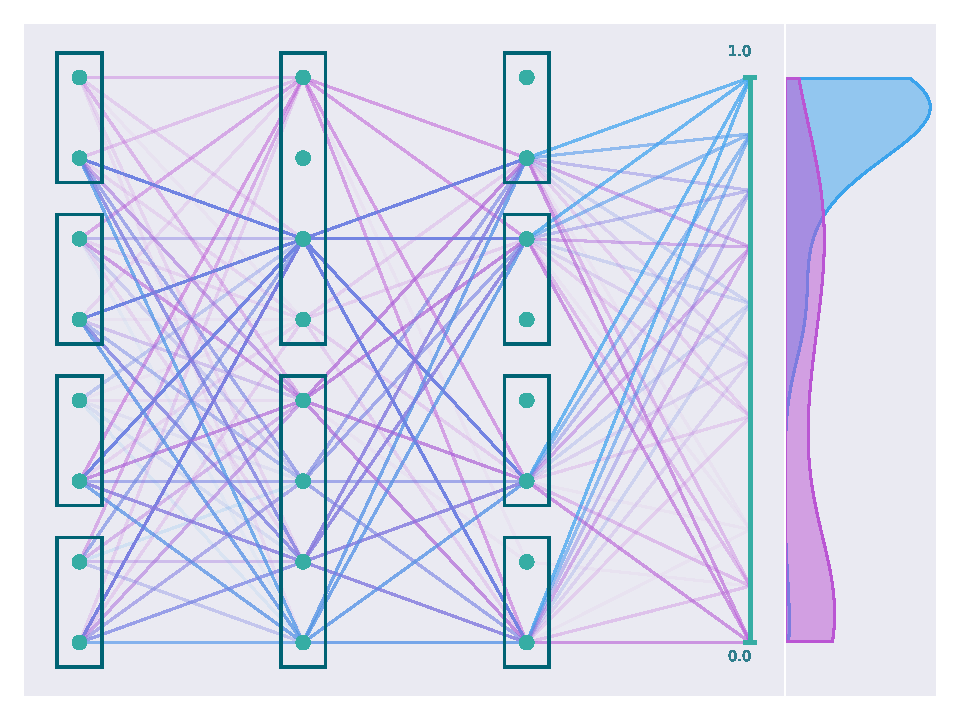
\includegraphics[width = 0.475\textwidth]{figures/NetworkVis/AfterTraining.pdf}
        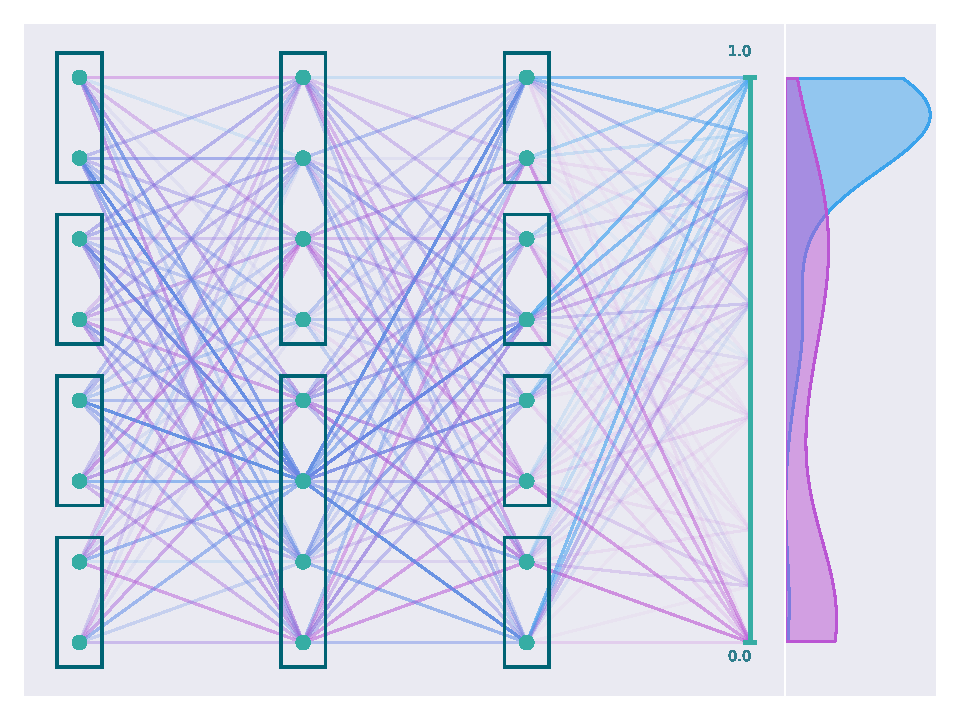
\includegraphics[width = 0.475\textwidth]{figures/NetworkVis/SCO/AfterTraining.pdf}
    \end{center}
\end{frame}
\begin{frame}{Ensemble network architecture}
    \vfill
    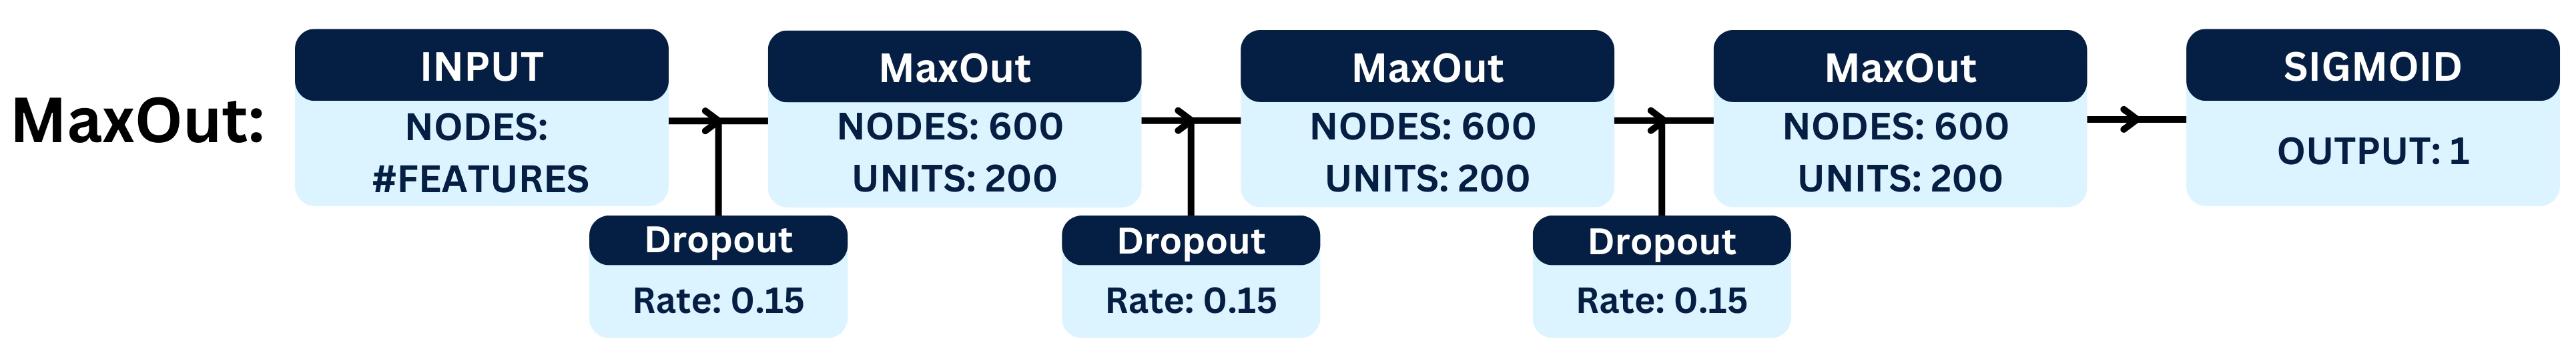
\includegraphics[width = 0.98\textwidth]{figures/maxout.png}
\end{frame}
\begin{frame}{Comparing sensitivity of channel-out, SCO and maxout}
    \begin{textblock}{1}(-0.0375, 0.2)
        \begin{itemize}
            \item Maxout: 24/30
            \item SCO: 6/30
            \begin{itemize}
                \item No trend for \\
                preferred masses
                \item Possibly improve\\
                      without layer on \\
                      prediction 
            \end{itemize}
        \end{itemize}
    \end{textblock}
    \begin{textblock}{1}(0.33, 0.2)
    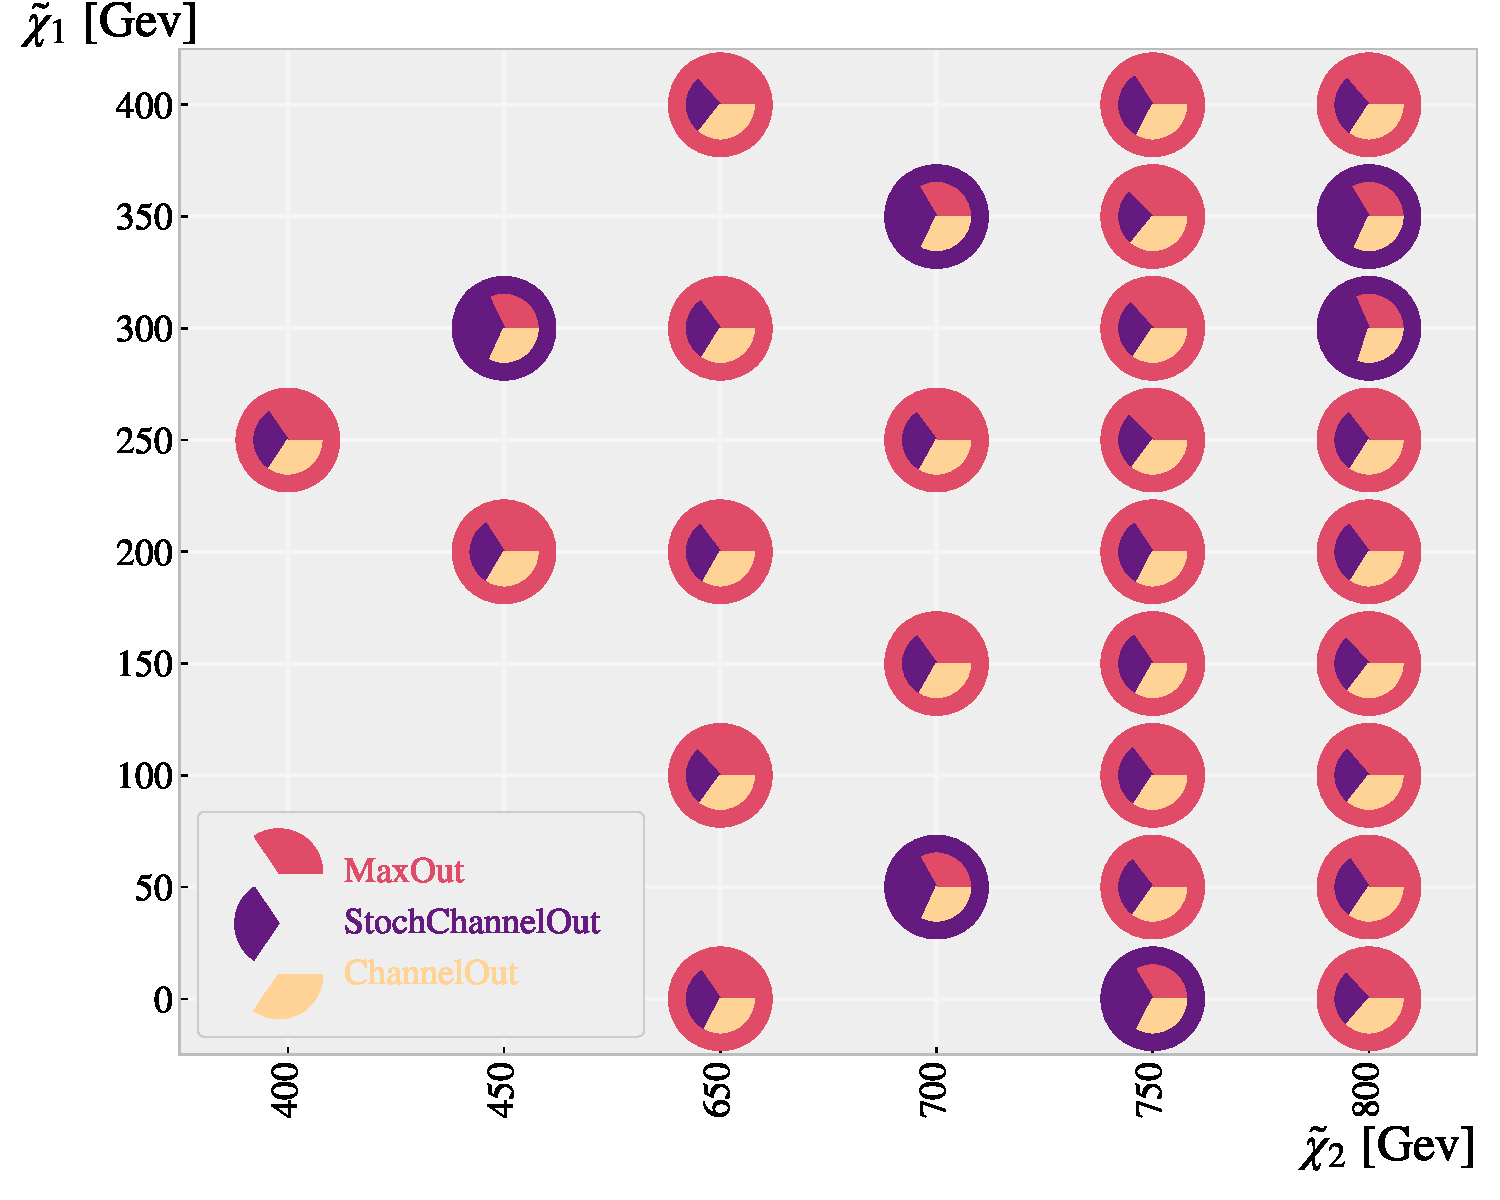
\includegraphics[width = 0.625\textwidth]{figures/Comps/EnsemblesNetworkComp.pdf}
    \end{textblock}
\end{frame}
% \begin{frame}
%     \begin{center}
%         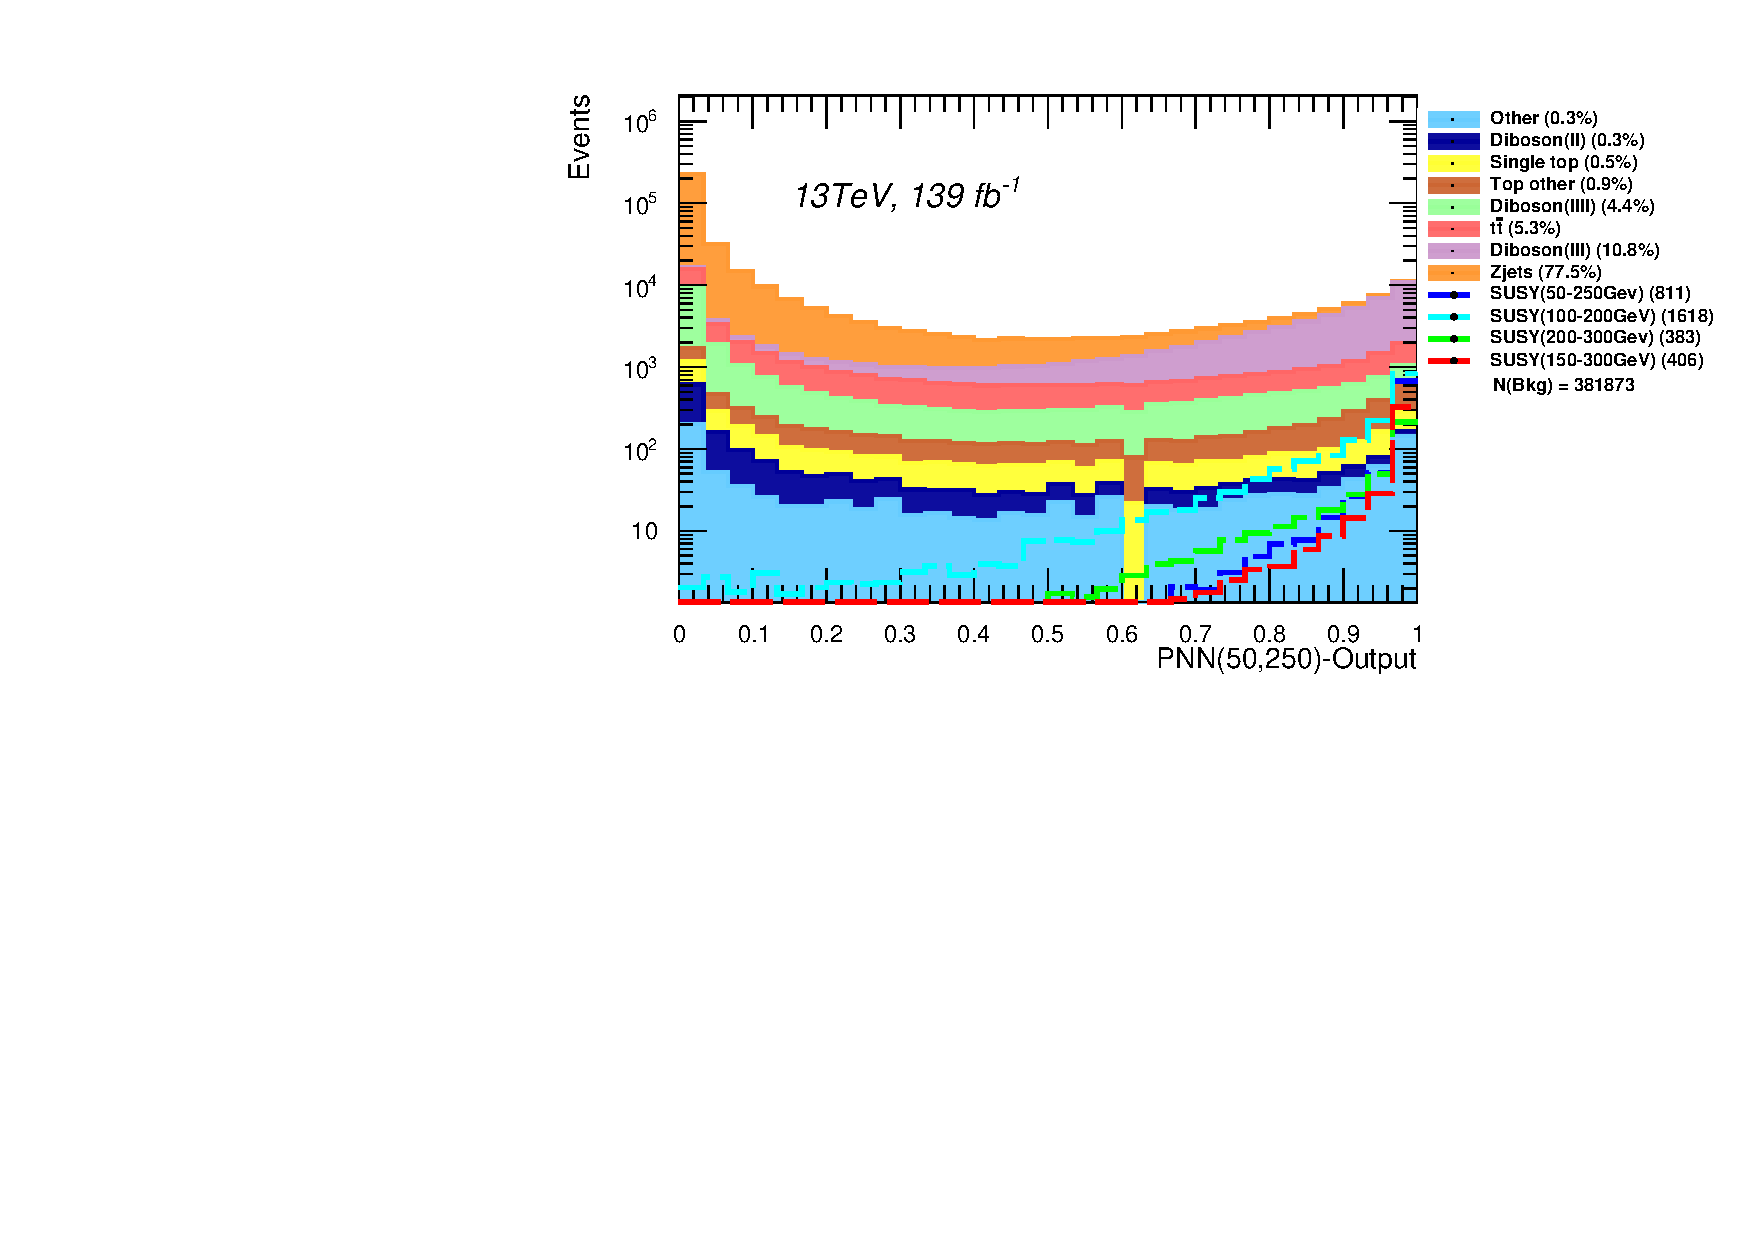
\includegraphics[width = 0.475\textwidth]{figures/PNN/PNN50250Dist.pdf}
%         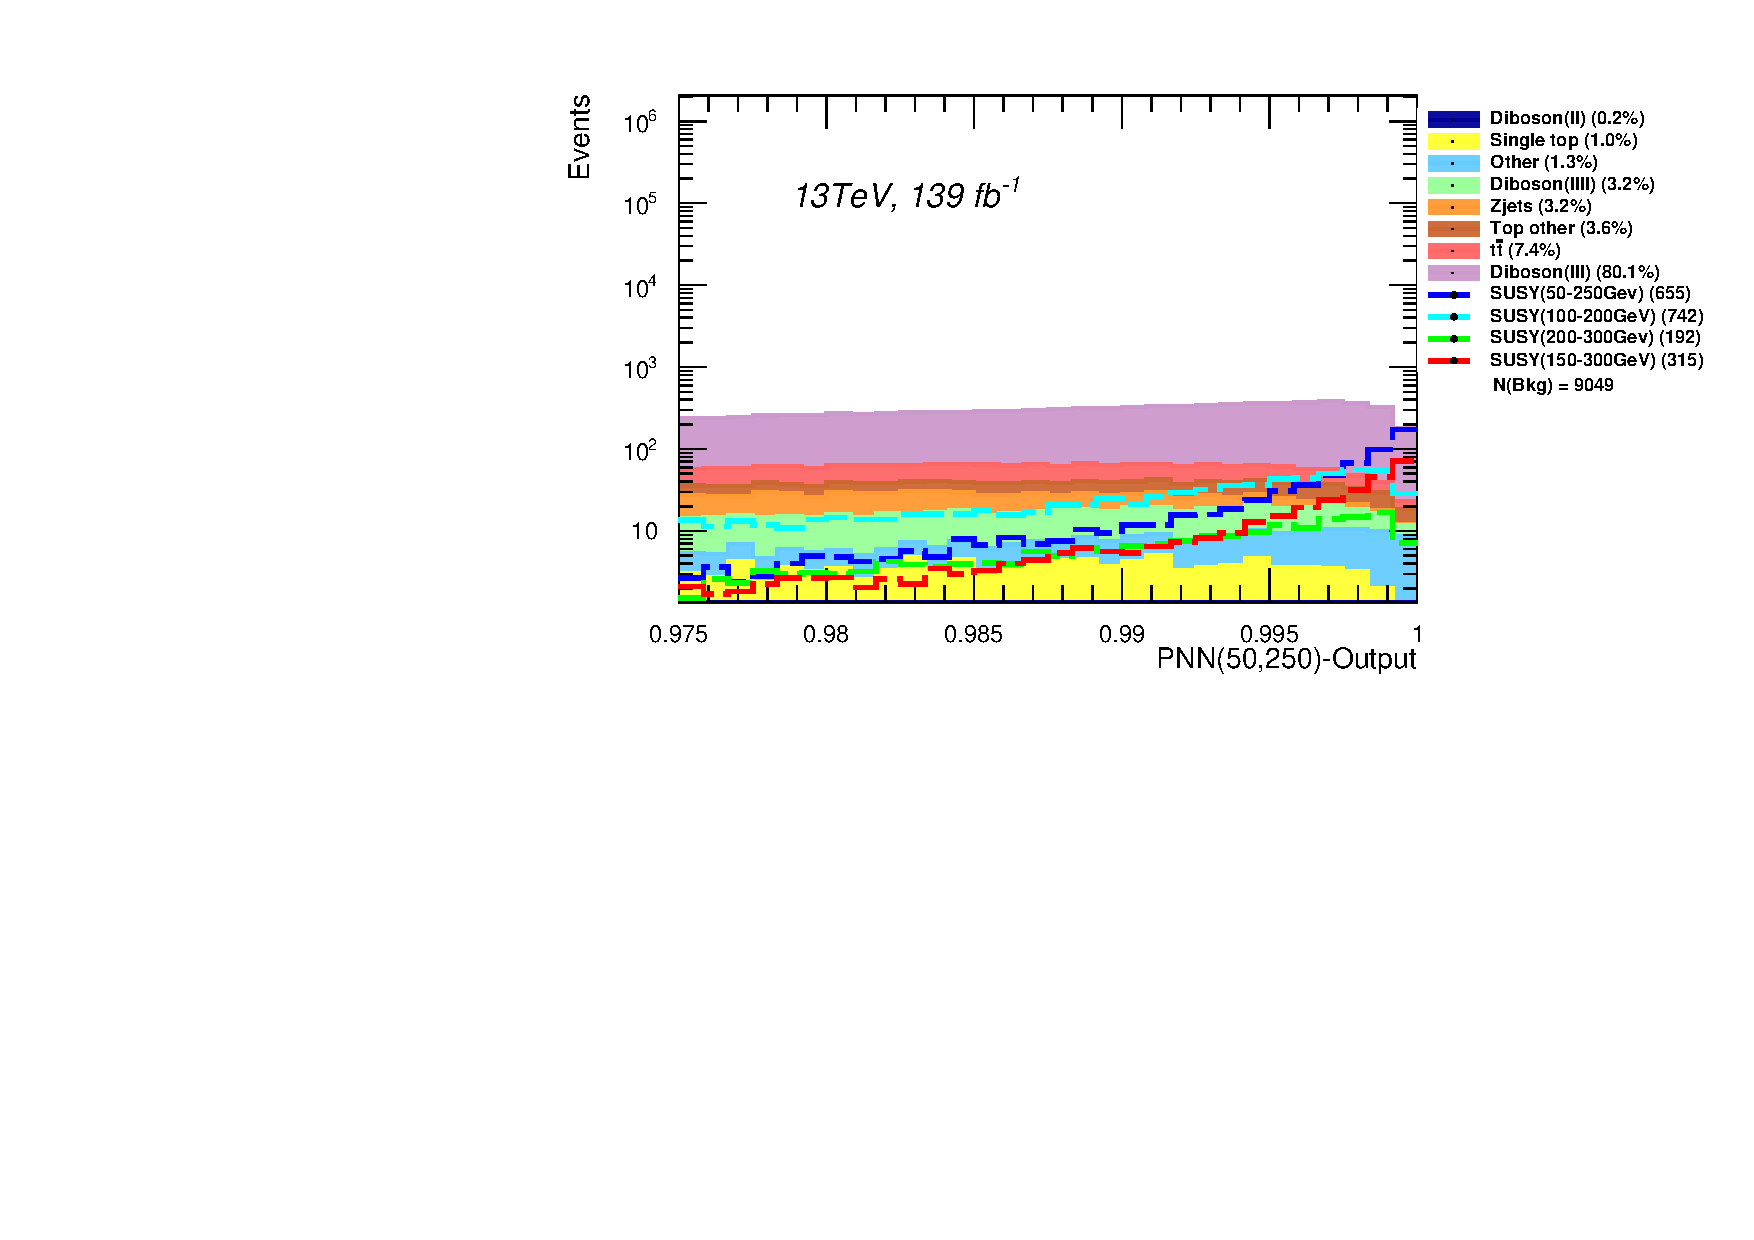
\includegraphics[width = 0.475\textwidth]{figures/PNN/PNN50250Dist_C7.pdf}
%     \end{center}
%     \begin{center}
%         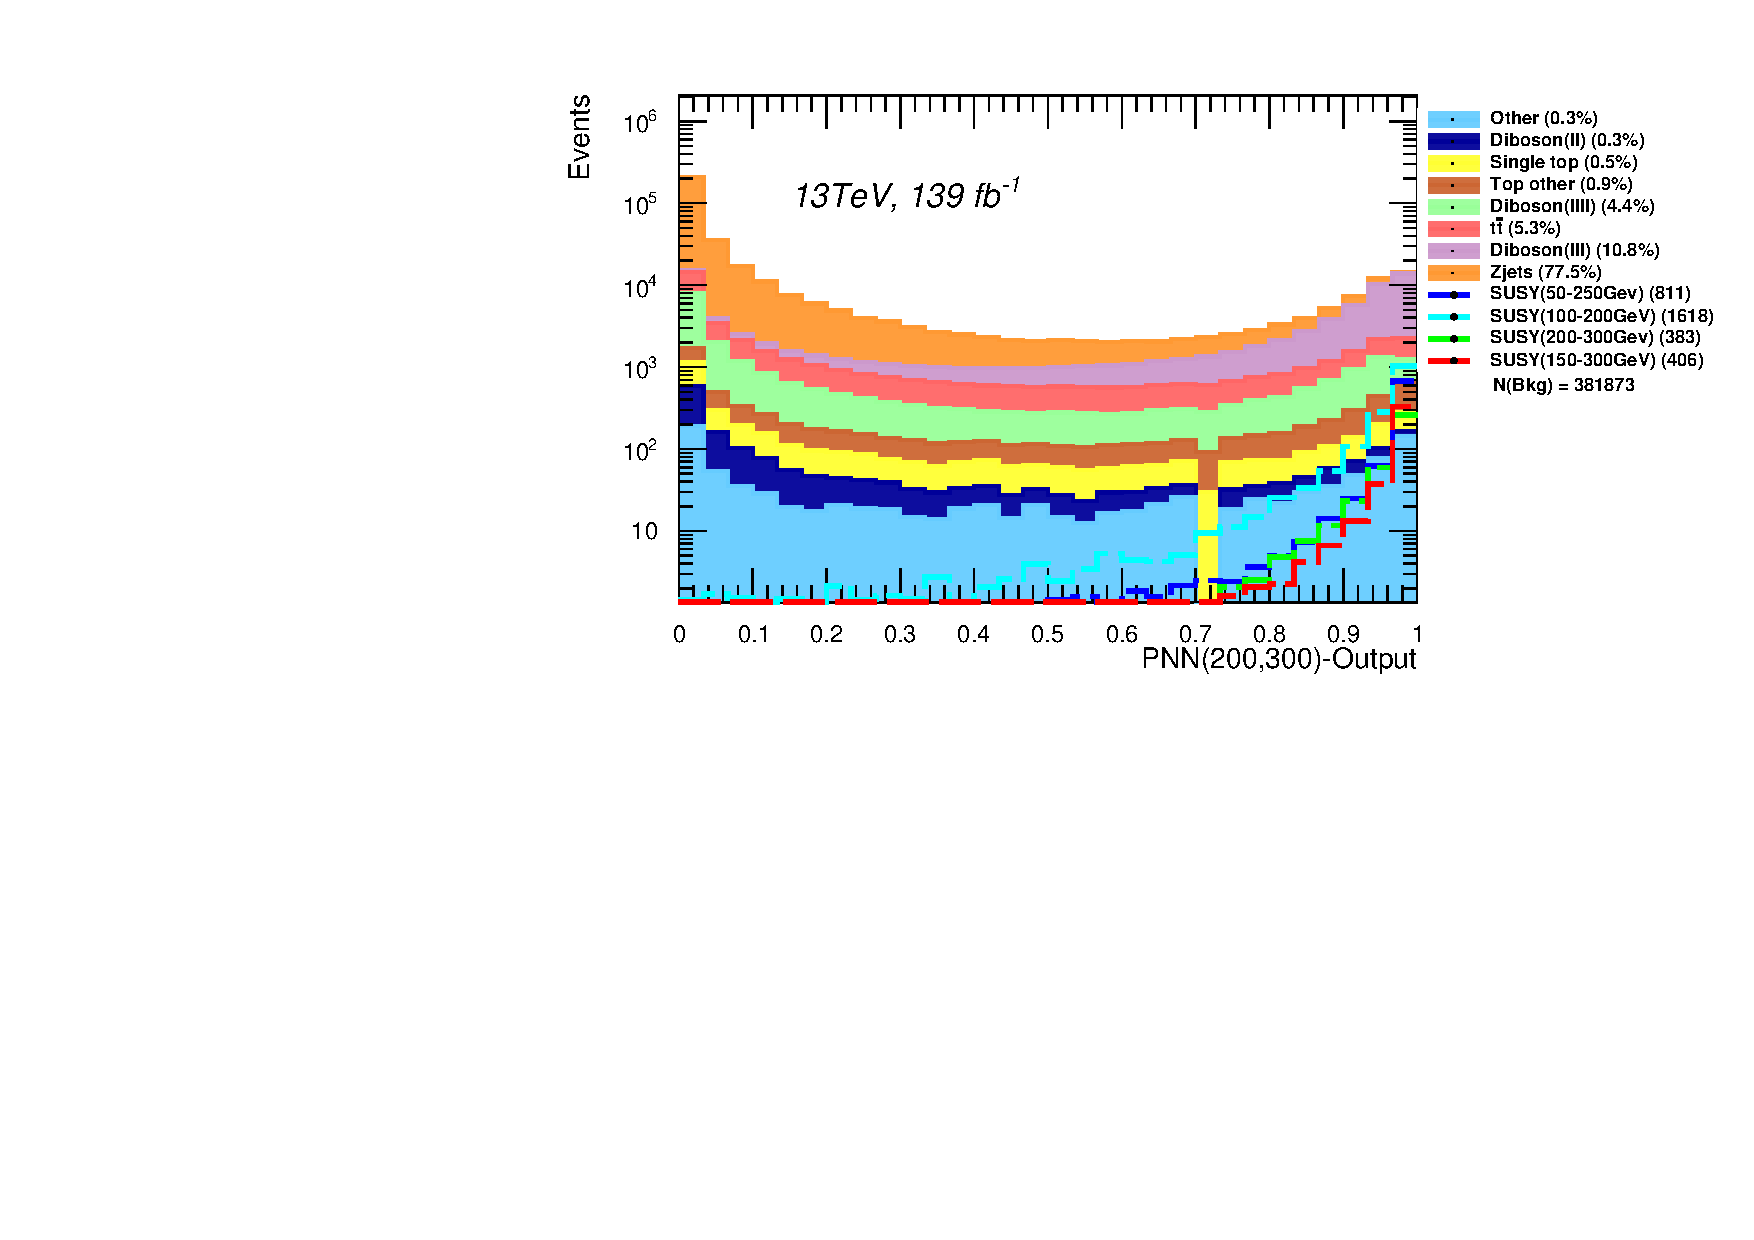
\includegraphics[width = 0.475\textwidth]{figures/PNN/PNN200300Dist.pdf}
%         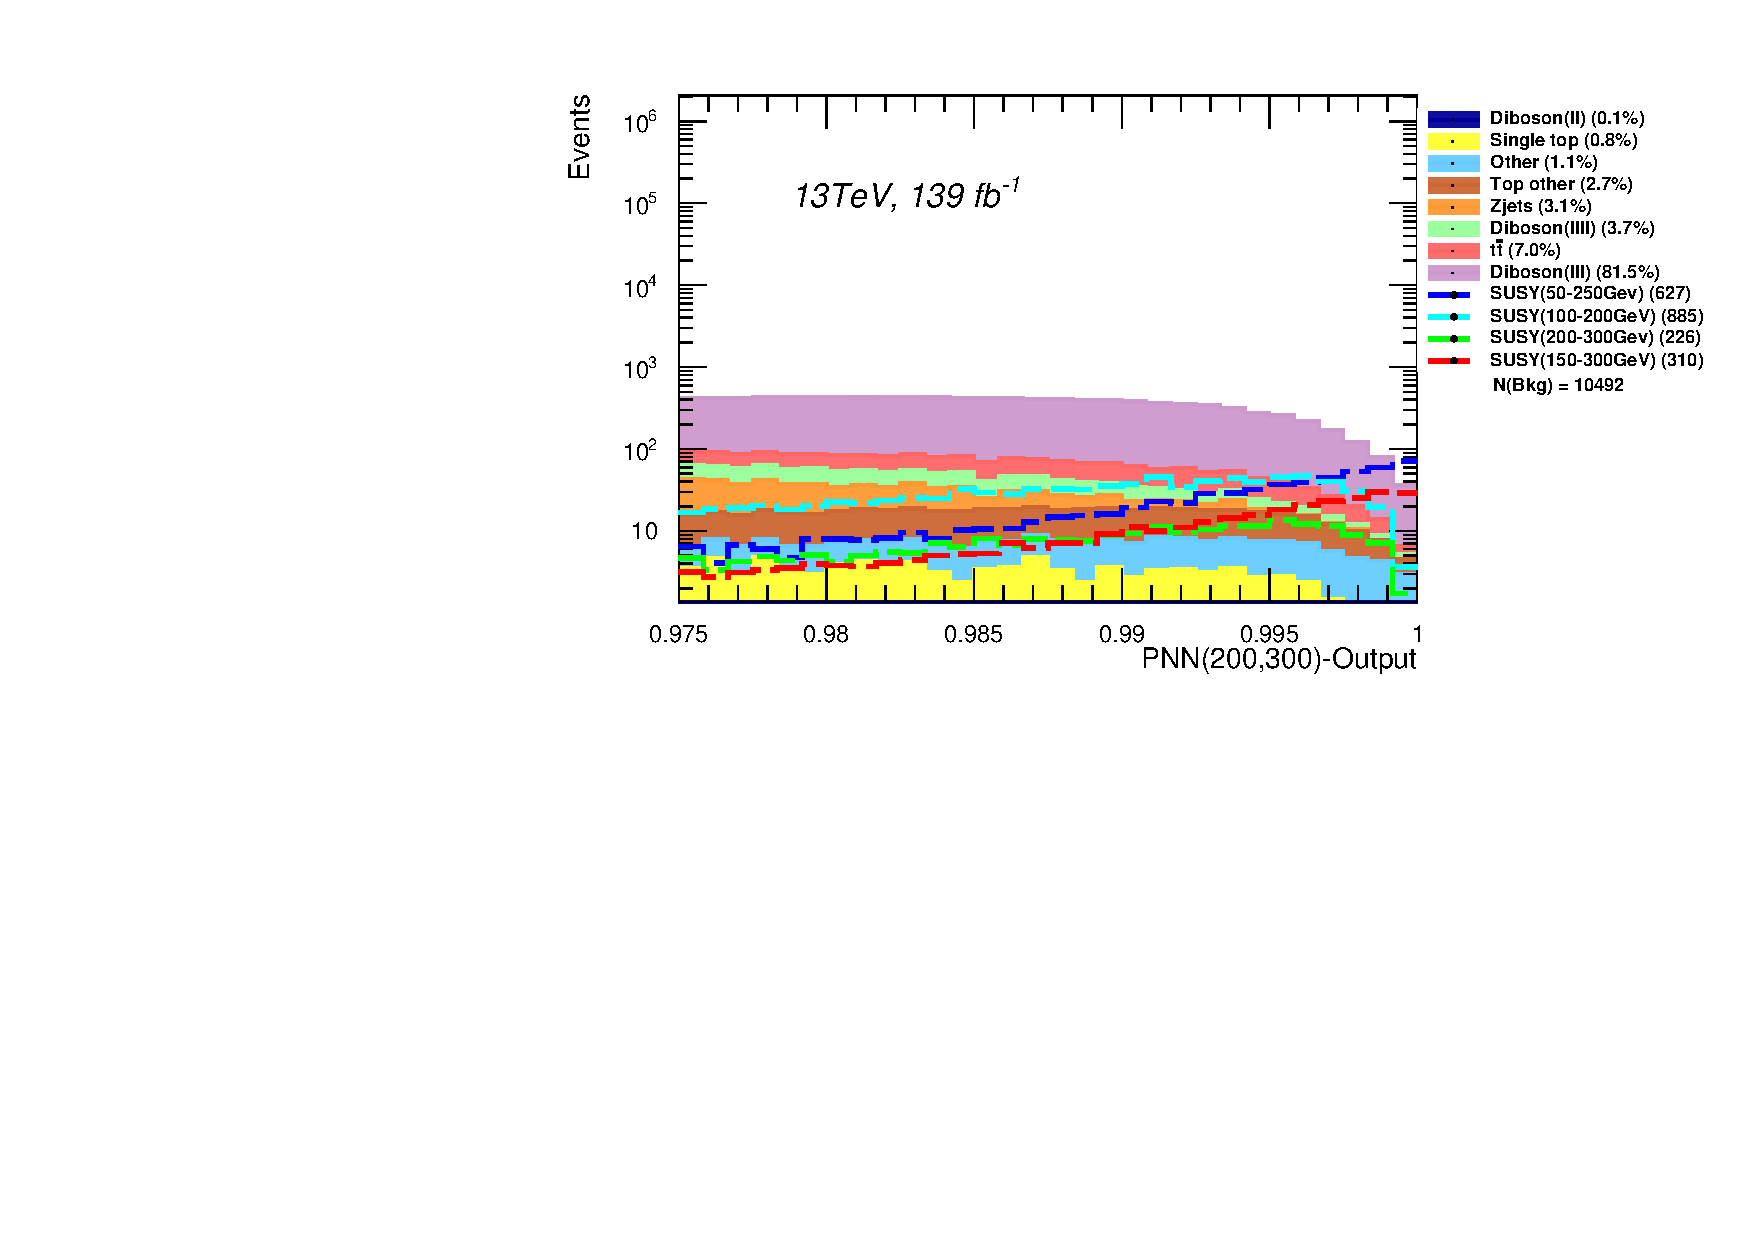
\includegraphics[width = 0.475\textwidth]{figures/PNN/PNN200300Dist_C7.pdf}
%     \end{center}
% \end{frame}

% \begin{frame}{Efficiency table}
%     \vfill
%     \begin{table}
%         \scriptsize
%         \centering
%         $
%         \begin{array}{cccccc}
%             \hline \text { \diagbox{\textbf{Parameters}}{\textbf{Channel}} }  & \text {$(50,250)$} & \text {$(100,200)$} & \text {$(150,300)$} & \text {$(200,300)$} & \text {$(Background)$} \\
%             \hline \text {$(50,250)$}   & \text { $\bf{80.8}\%$ } & \text { $45.8\%$ } & \text { $\bf{77.5}\%$ } & \text { $50.1\%$ } & \text { $2.4\%$ }  \\
%             \text {$(200,300)$}   & \text { $77.3\%$ } & \text { $\bf{54.6}\%$ } & \text { $76.3\%$ } & \text { $\bf{59.0}\%$ } & \text { $2.74\%$ }\\
%             \hline
%         \end{array}
%         $
%     \end{table}
% \end{frame}

\begin{frame}{Comparing the sensitivity on a subset of the signal}
    \begin{textblock}{1}(0.12, 0.175)
    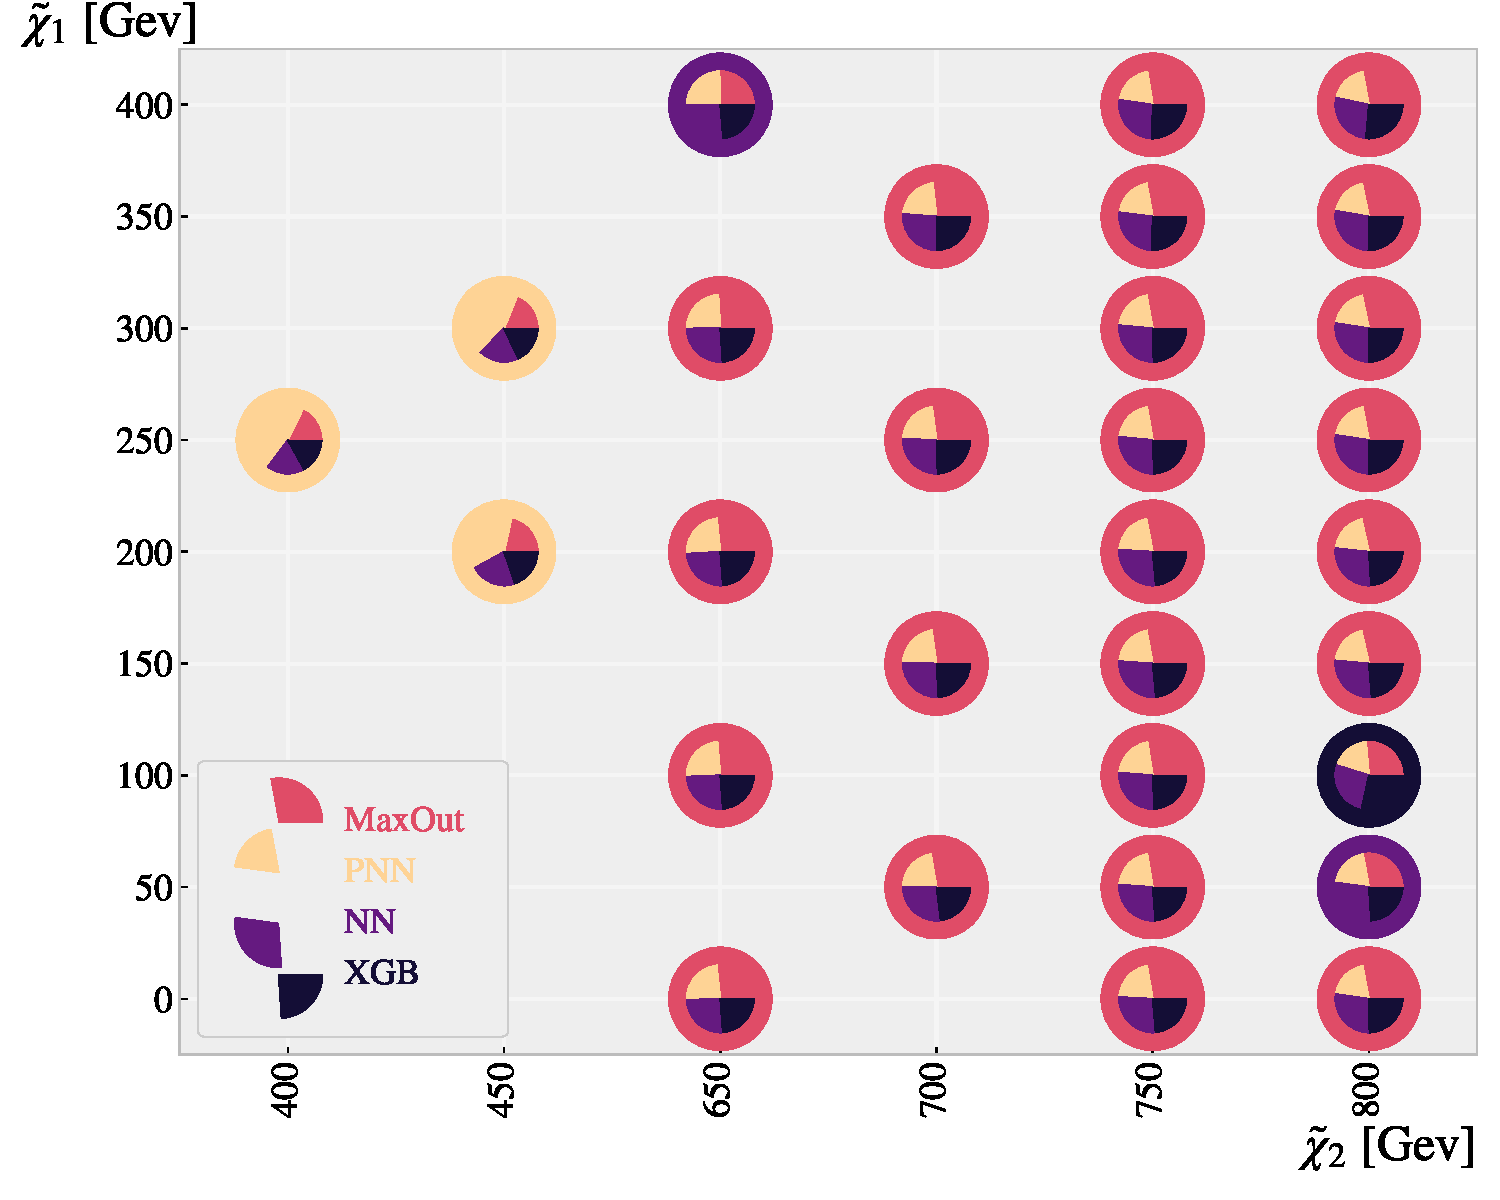
\includegraphics[width=0.7\textwidth]{figures/Comps/GenPlussXGBNetworkComp.pdf}
    \end{textblock}
    % \begin{textblock}{0.4}(-0.02, 0.175)
    %     \begin{itemize}
    %         \item NN vs BDT
    %         \item Maxout achieves highest sensitivity
    %         \item PNN very sensitive for low masses 
    %         \item Maxout sensitive for high masses 
    %         \begin{itemize}
    %             \item Long-term memory
    %         \end{itemize}
    %     \end{itemize}
    % \end{textblock}
\end{frame}

\begin{frame}{Increasing sensitivity through a PCA}
    \begin{itemize}
        \item Dimensionality reduction
        \item This analysis
        \begin{itemize}
            \item Demand conservation of $99.9\%$ of variance/spread
            \item 5 features removed
        \end{itemize}
    \end{itemize}
    \begin{textblock}{0.8}(0.02, 0.6)
        {Maxout}
    \end{textblock}
    \begin{textblock}{0.8}(0.9, 0.6)
        {PNN}
    \end{textblock}
    \vfill
    \begin{center}
        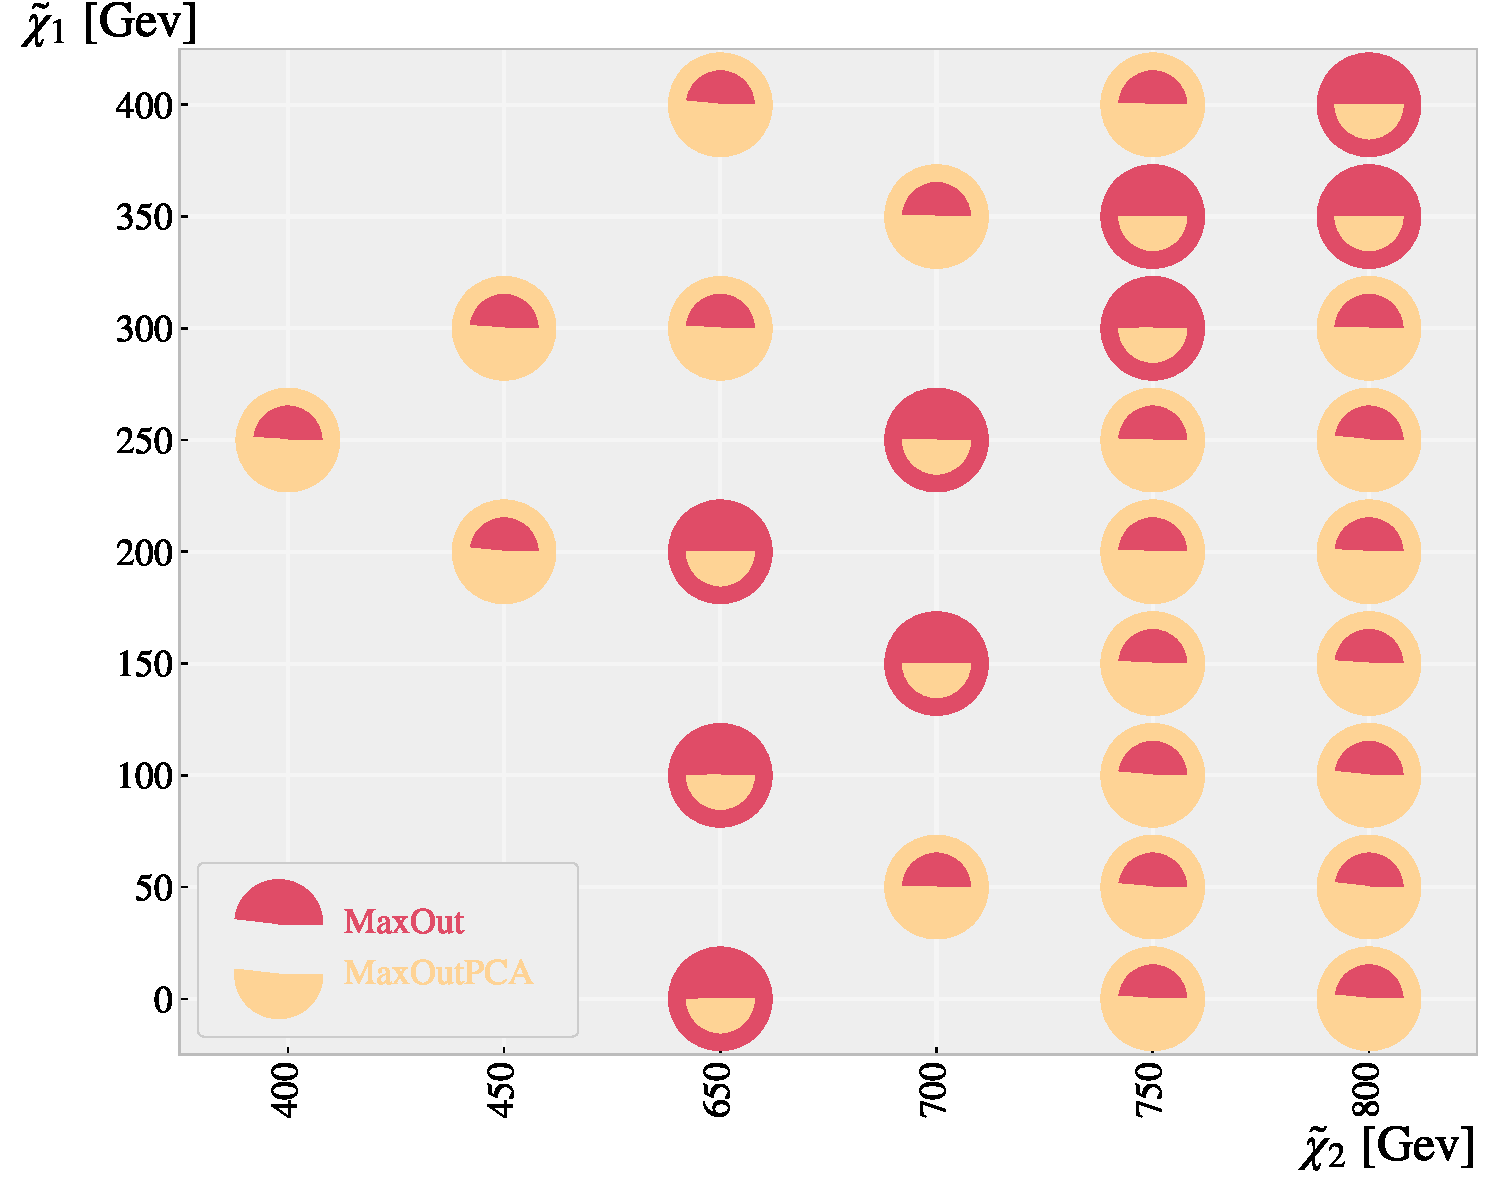
\includegraphics[width=0.415\textwidth]{figures/Comps/MaxOutPCANetworkComp.pdf}
        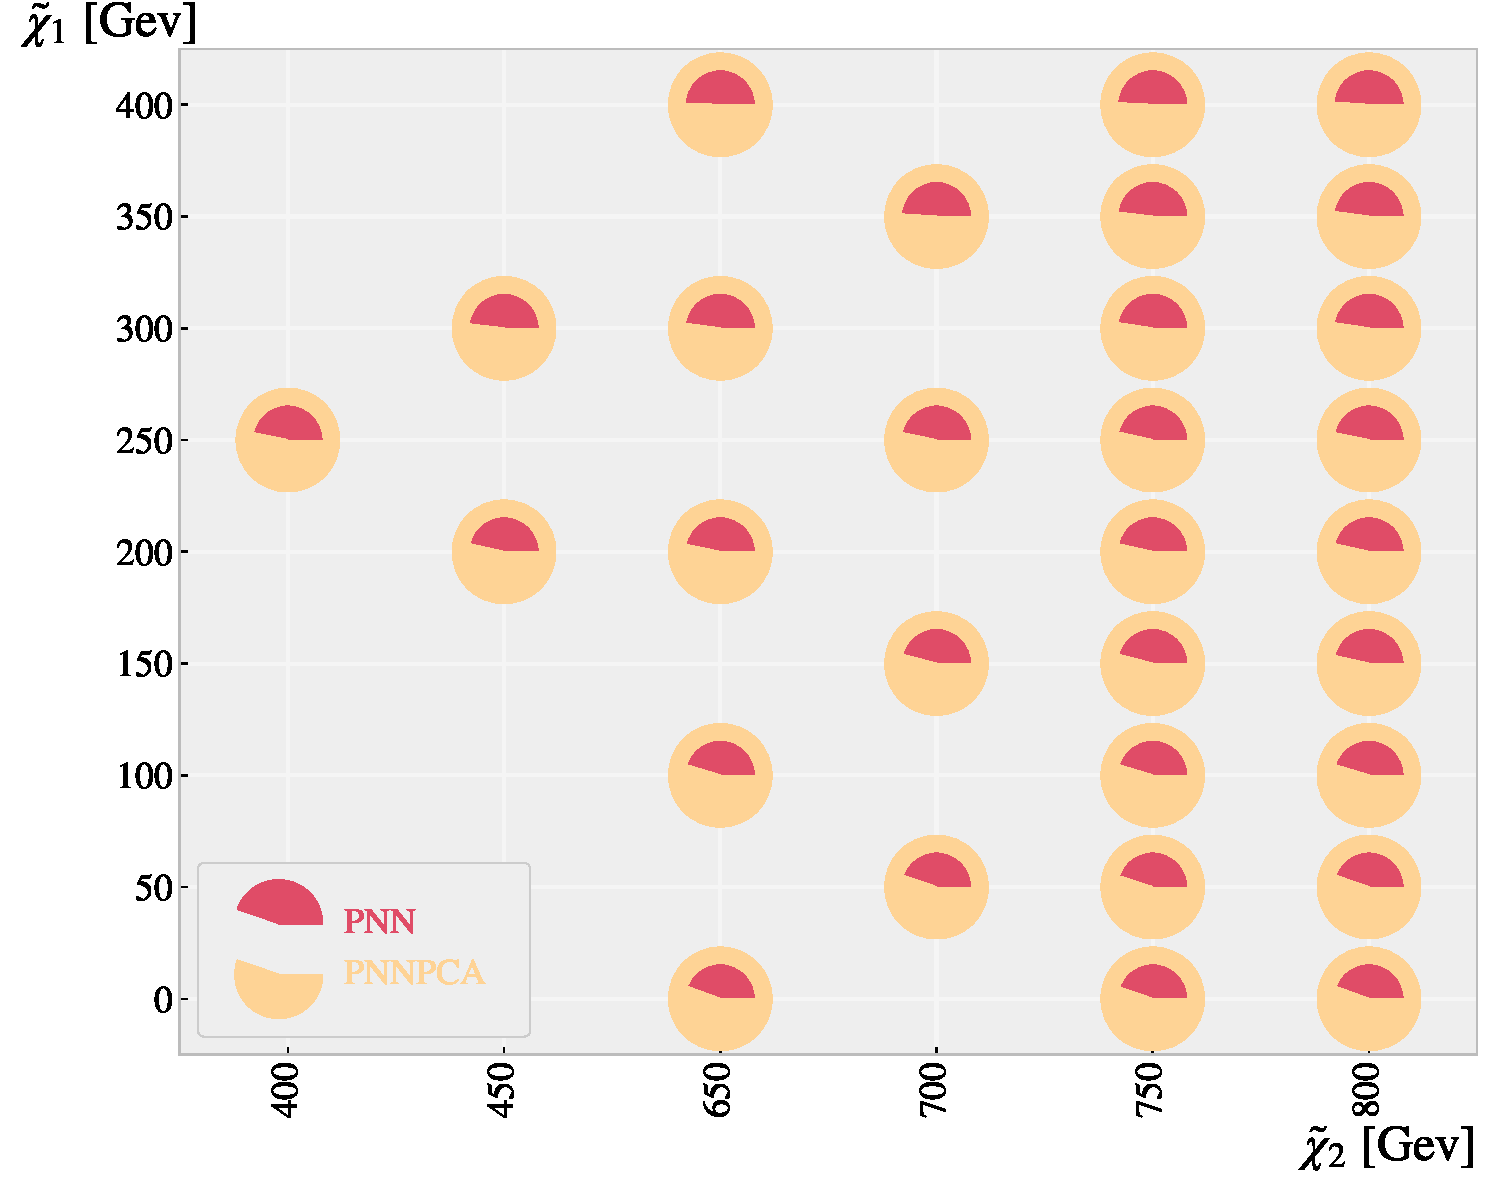
\includegraphics[width=0.415\textwidth]{figures/Comps/PNNPCANetworkComp.pdf}
    \end{center}
\end{frame}


% \begin{frame}{Comparing the methods to previous analysis}
%     \begin{itemize}
%         \item Compare the expected limits of three best models
%               to analysis made by ATLAS in 2021 \cite{atlas_search_2021}
%         \item Introduce flat uncertainty for realistic comparison ($20\%$, $10\%$, $<1\%$) 
%         \item Include top performing methods
%         \begin{itemize}
%             \item Maxout model with PCA
%             \item PNN with PCA
%             \item Ordinary dense neural network without PCA
%         \end{itemize}
%     \end{itemize}
% \end{frame}
\begin{frame}{Comparing methods on full signal grid}
    \centering
    \vfill
    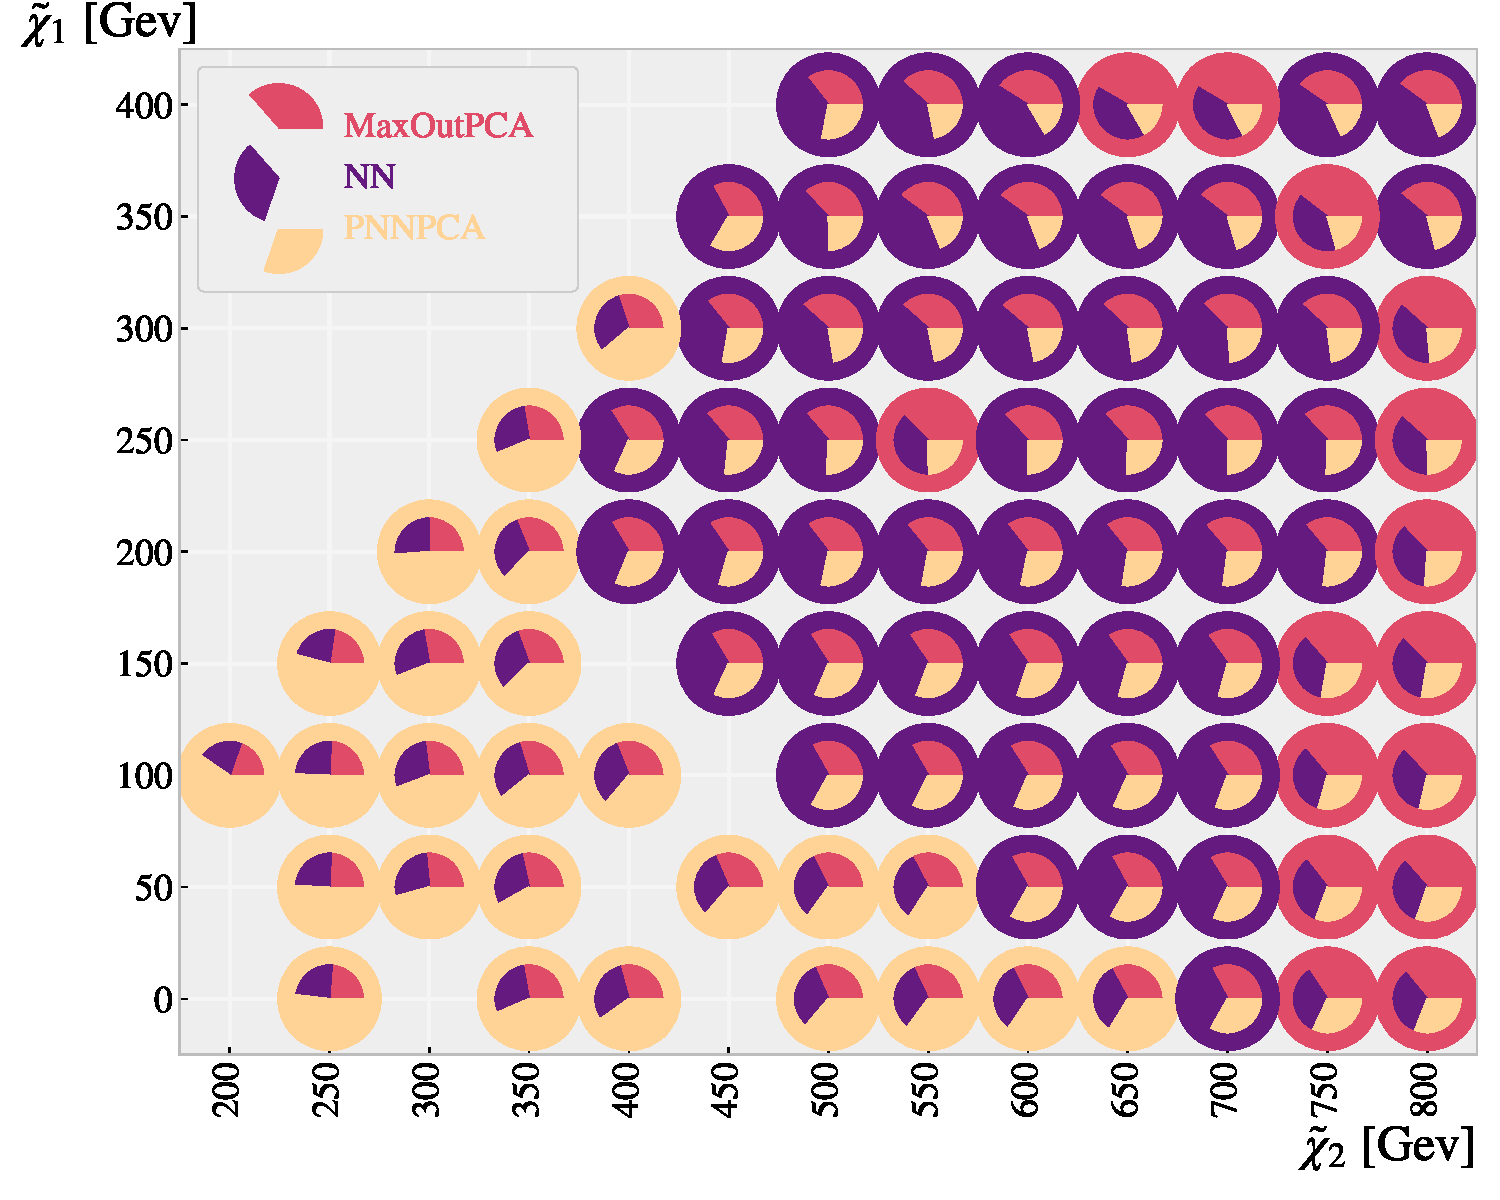
\includegraphics[width = 0.8\textwidth]{figures/Comps/FS_MLMNetworkComp.pdf}
\end{frame}
\begin{frame}{Comparing the methods to previous analysis}
    \begin{textblock}{1}(0.4,.15)
    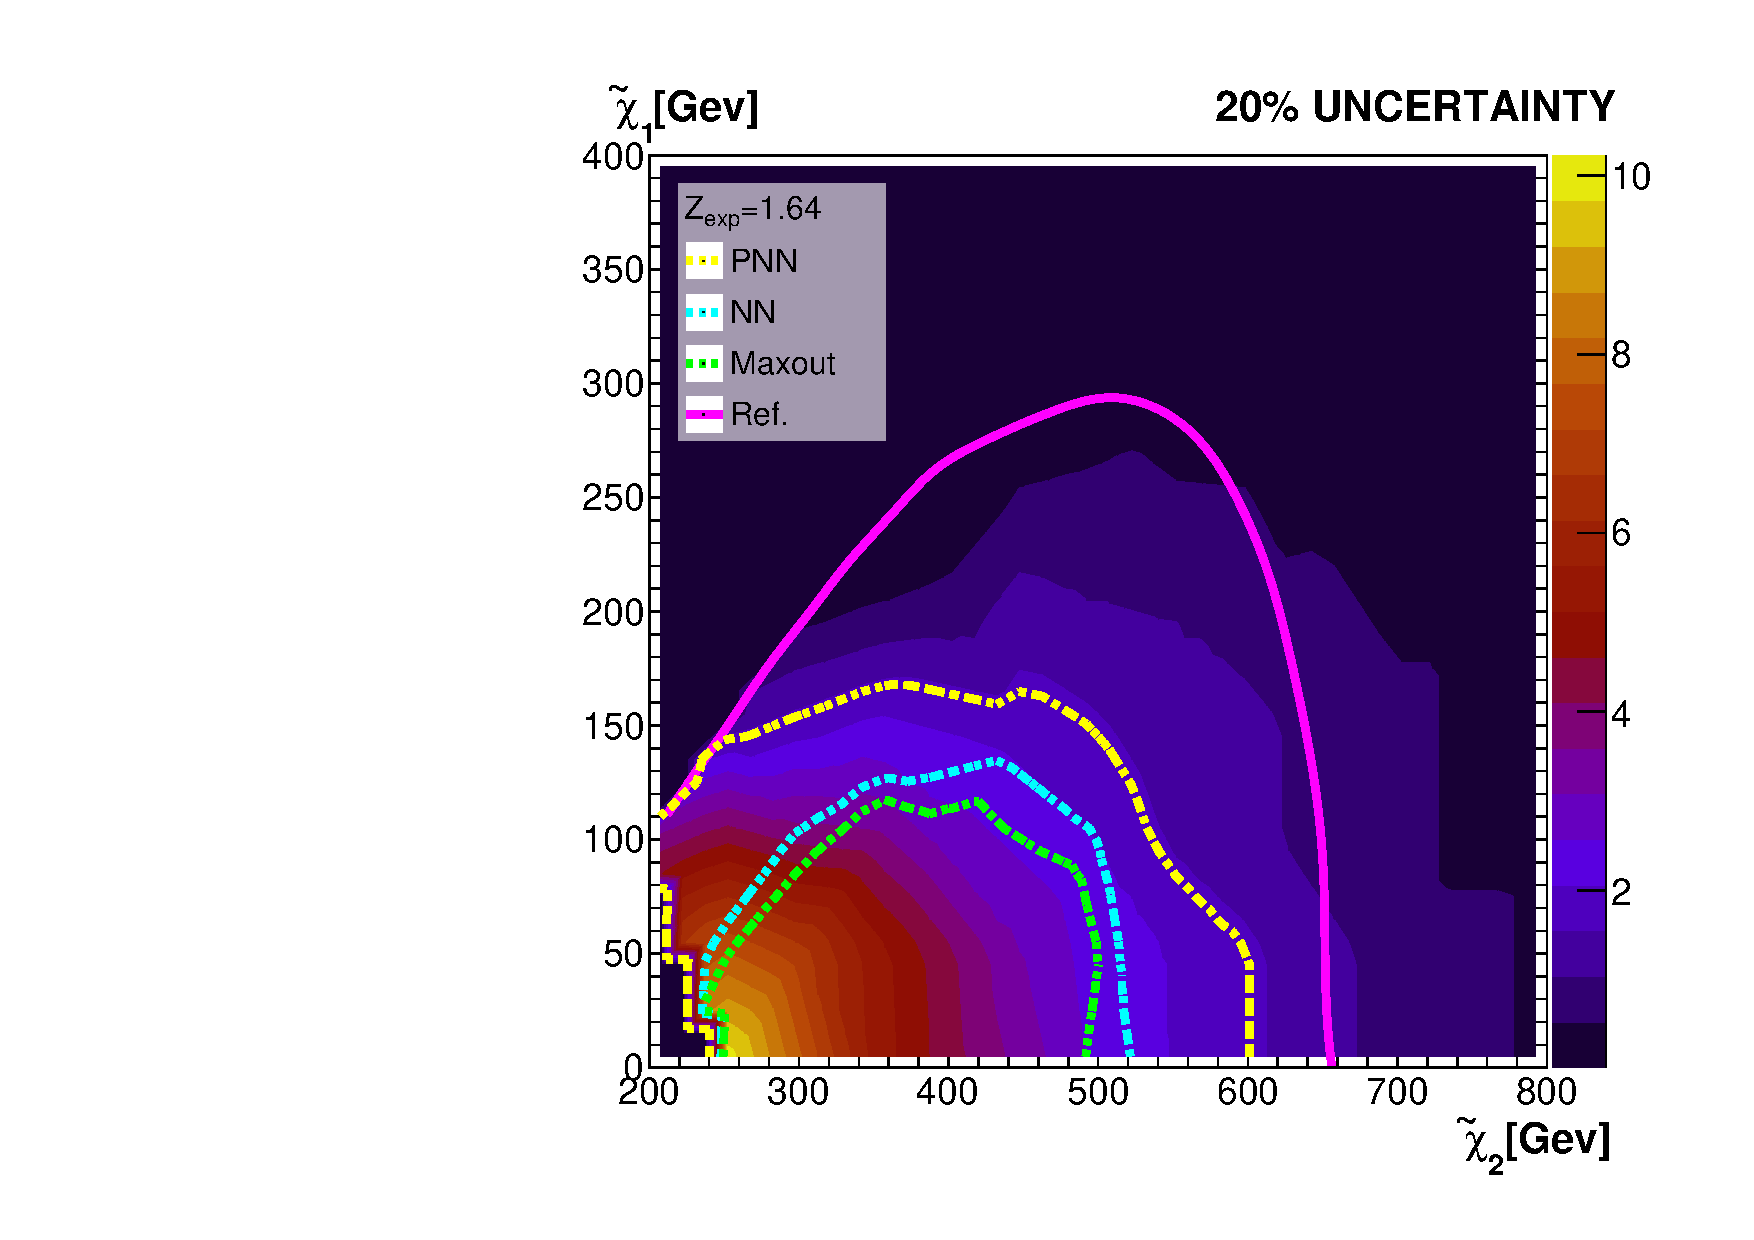
\includegraphics[width=0.6\textwidth]{figures/Limits/compLimit20.pdf}
    \end{textblock}
    \begin{textblock}{1}(0.54,.39)
        \scriptsize
        \cite{atlas_search_2021}
    \end{textblock}
    \begin{textblock}{.45}(-0.03,.2)
    \begin{itemize}
        \item Compare the expected limits to analysis made by ATLAS in 2021 \cite{atlas_search_2021}
        \item Introduce flat uncertainty ($20\%$, $10\%$, $<1\%$) 
        \item Why not better sensitivity?
    \end{itemize}
\end{textblock}
\end{frame}
% \begin{frame}
%     \vfill
%     \centering
%     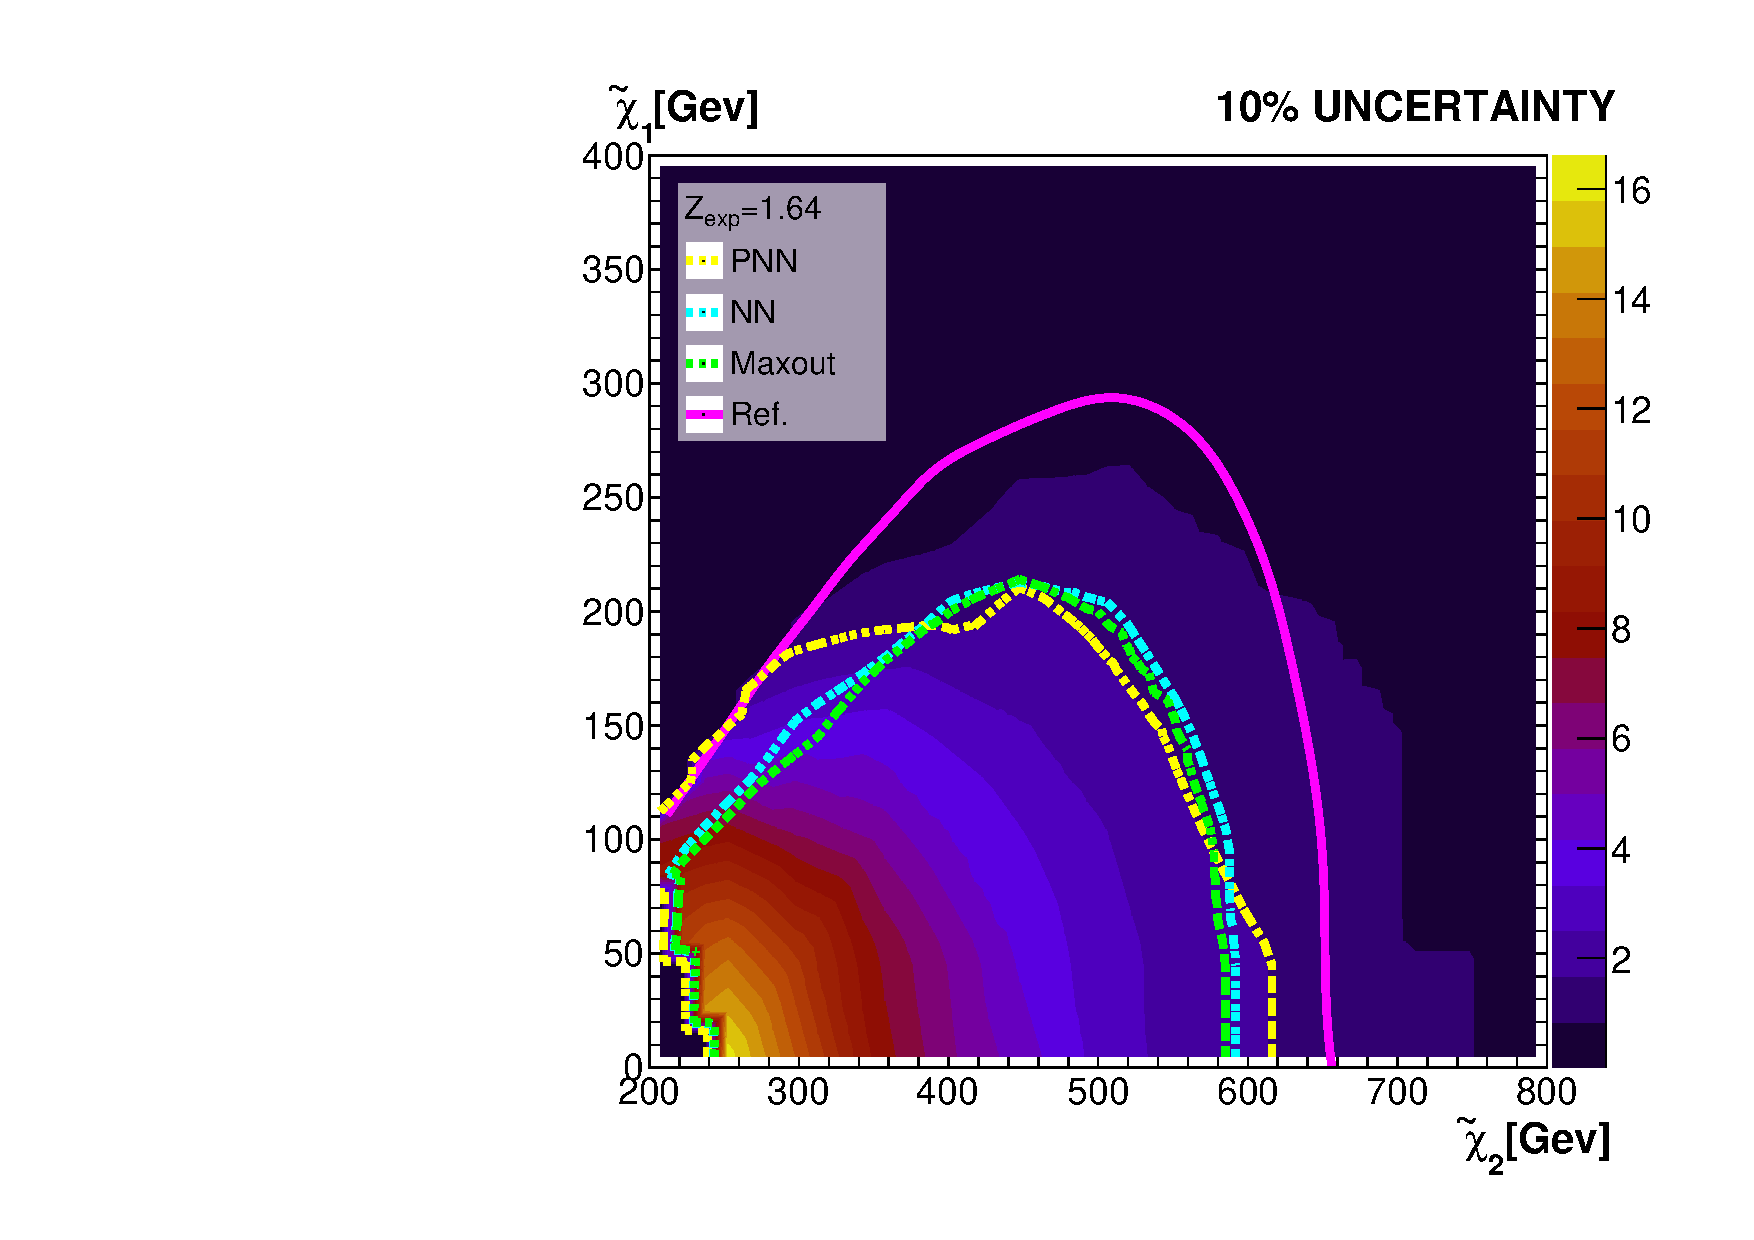
\includegraphics[width=0.45\textwidth]{figures/Limits/compLimit10.pdf}
%     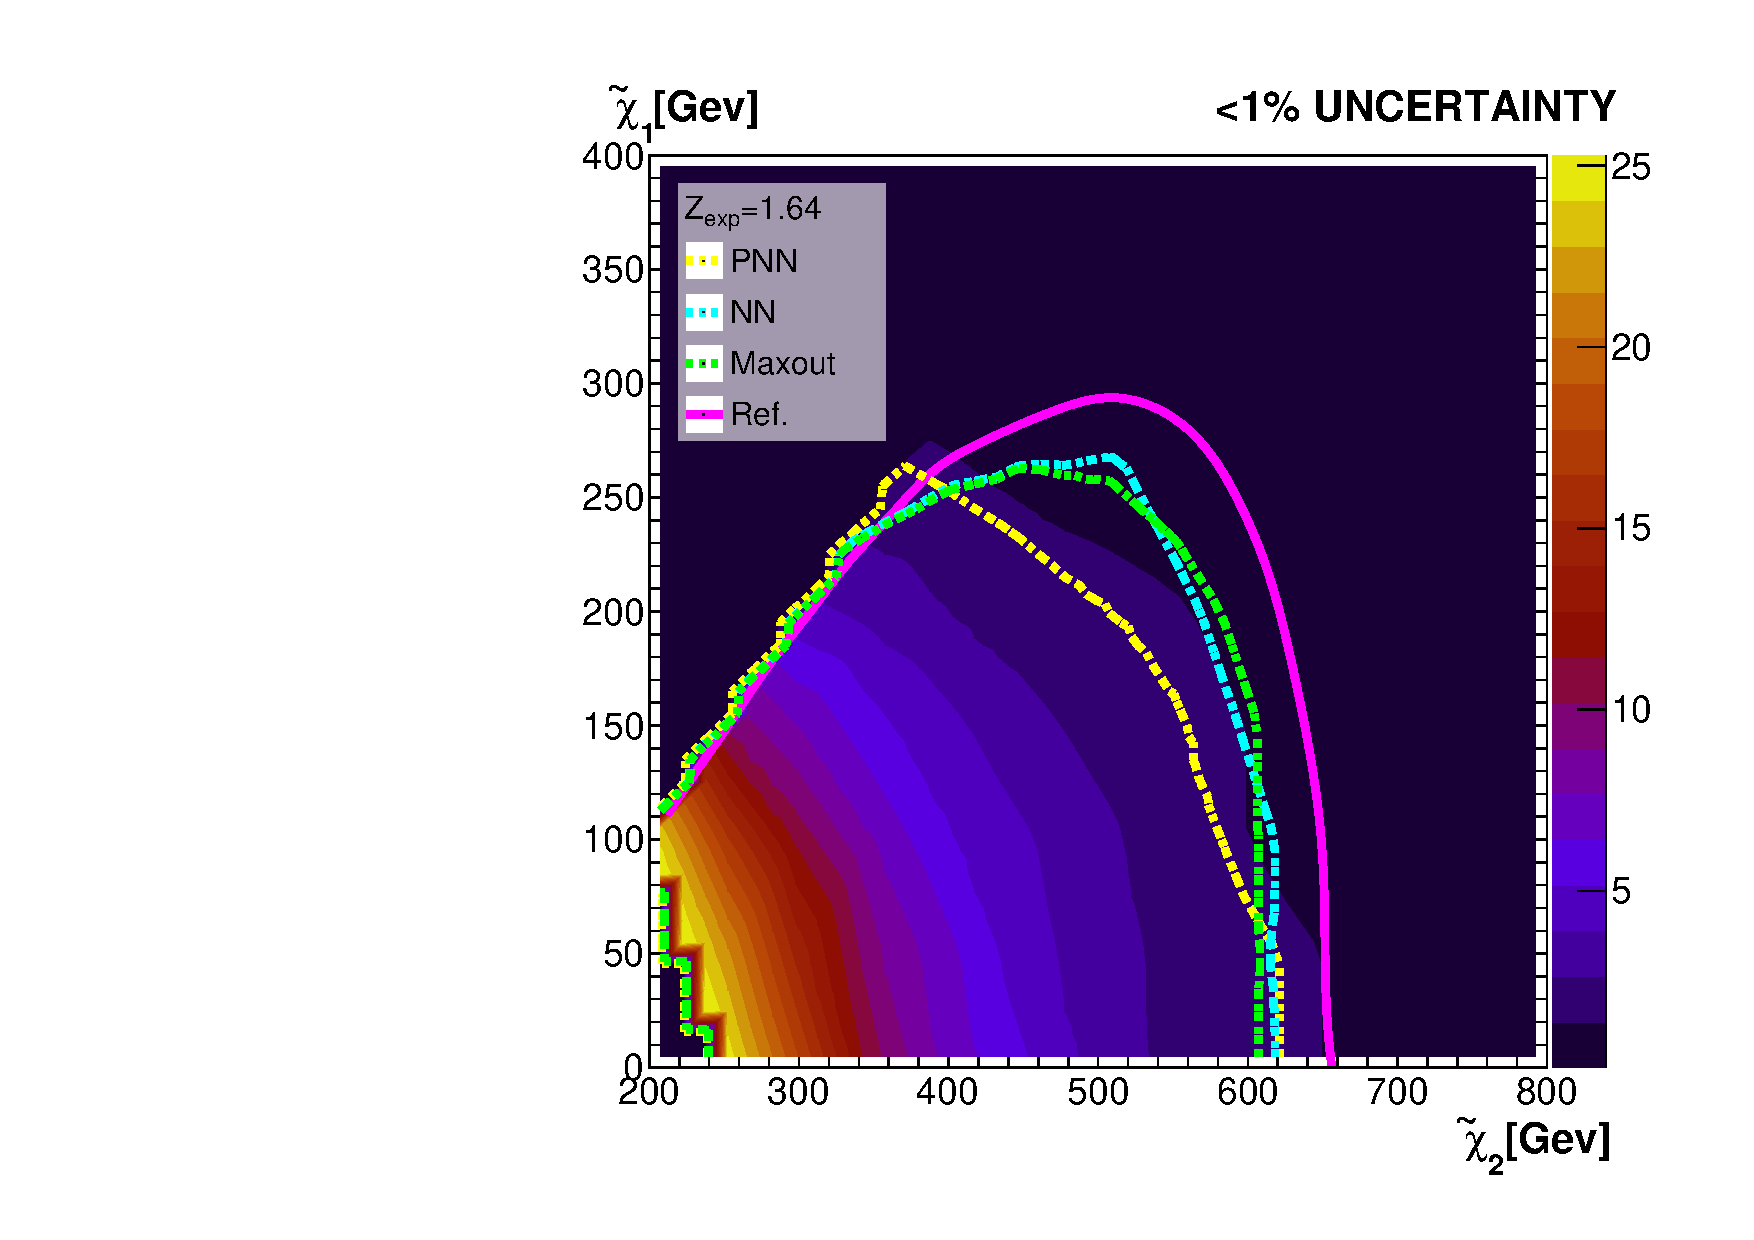
\includegraphics[width=0.45\textwidth]{figures/Limits/compLimit1.pdf}
%     \begin{textblock}{1}(-0.32,.39)
%         \tiny
%         \cite{atlas_search_2021}
%     \end{textblock}
%     \begin{textblock}{1}(0.112,.39)
%         \tiny
%         \cite{atlas_search_2021}
%     \end{textblock}
% \end{frame}
\section{Conclusion $\&$ Outlook}
\begin{frame}{Conclusion $\&$ Outlook}
    \tableofcontents[currentsection]
\end{frame}
\begin{frame}{Conclusion $\&$ Outlook}
    \begin{enumerate}
        \item Including a diverse signal set can improve performance
        \item The LWTA layers improve long-term memory via pattern specific pathways
        \item PCA increased sensitivity of PNN and maxout model in original signal set
        \item None of the networks extended expected limit past previous ATLAS analysis
        \item PNN exhibited bias towards lower masses, whereas maxout model achieved a more balanced 
              sensitivity
        \item Long-term memory of LWTA layers is promising in future analysis where higher masses are studied 
    \end{enumerate}
\end{frame}





\begin{frame}{References}
    \begin{thebibliography}{}
        \scriptsize
        \setbeamertemplate{bibliography item}[online]
        \bibitem{Maximilien}
        Maximilien Brice.
        \newblock \enquote{Installing the ATLAS calorimeter. Vue centrale du
        détecteur ATLAS avec ses huit toroides entourant le
        calorimètre avant son déplacement au centre du
        détecteur}.
        \newblock \url{https://cds.cern.ch/record/910381}
        \newblock Figure on front page

        \bibitem{Maximilien}
        Joao Pequenao.
        \newblock \enquote{Event Cross Section in a computer generated image of the ATLAS detector.}.
        \newblock \url{https://cds.cern.ch/record/1096081}
        \newblock Figure on slide 3

        \bibitem{Collision}
        ATLAS Collaboration.
        \newblock \enquote{ATLAS event at 900 GeV - 6 May 2015 - Run 264034 lb 659
        event 11526514}.
        \newblock \url{https://cds.cern.ch/record/2015238}
        \newblock Figure on slide 4

        \setbeamertemplate{bibliography item}[article]
        \bibitem{atlas_search_2021}
        ATLAS Collaboration [4].
        \newblock \enquote{Search for chargino--neutralino pair production in final states with three leptons and missing transverse momentum in {$\sqrt{s}$} = 13 {TeV} pp collisions with the {ATLAS} detector}.
        \newblock \url{http://arxiv.org/abs/2106.01676}

    \end{thebibliography}
\end{frame}


\end{document}